
\documentclass{article} % For LaTeX2e
\usepackage{iclr2027_conference,times}

% Optional math commands from https://github.com/goodfeli/dlbook_notation.
%%%%% NEW MATH DEFINITIONS %%%%%

\usepackage{amsmath,amsfonts,bm}

% Mark sections of captions for referring to divisions of figures
\newcommand{\figleft}{{\em (Left)}}
\newcommand{\figcenter}{{\em (Center)}}
\newcommand{\figright}{{\em (Right)}}
\newcommand{\figtop}{{\em (Top)}}
\newcommand{\figbottom}{{\em (Bottom)}}
\newcommand{\captiona}{{\em (a)}}
\newcommand{\captionb}{{\em (b)}}
\newcommand{\captionc}{{\em (c)}}
\newcommand{\captiond}{{\em (d)}}

% Highlight a newly defined term
\newcommand{\newterm}[1]{{\bf #1}}


% Figure reference, lower-case.
\def\figref#1{figure~\ref{#1}}
% Figure reference, capital. For start of sentence
\def\Figref#1{Figure~\ref{#1}}
\def\twofigref#1#2{figures \ref{#1} and \ref{#2}}
\def\quadfigref#1#2#3#4{figures \ref{#1}, \ref{#2}, \ref{#3} and \ref{#4}}
% Section reference, lower-case.
\def\secref#1{section~\ref{#1}}
% Section reference, capital.
\def\Secref#1{Section~\ref{#1}}
% Reference to two sections.
\def\twosecrefs#1#2{sections \ref{#1} and \ref{#2}}
% Reference to three sections.
\def\secrefs#1#2#3{sections \ref{#1}, \ref{#2} and \ref{#3}}
% Reference to an equation, lower-case.
\def\eqref#1{equation~\ref{#1}}
% Reference to an equation, upper case
\def\Eqref#1{Equation~\ref{#1}}
% A raw reference to an equation---avoid using if possible
\def\plaineqref#1{\ref{#1}}
% Reference to a chapter, lower-case.
\def\chapref#1{chapter~\ref{#1}}
% Reference to an equation, upper case.
\def\Chapref#1{Chapter~\ref{#1}}
% Reference to a range of chapters
\def\rangechapref#1#2{chapters\ref{#1}--\ref{#2}}
% Reference to an algorithm, lower-case.
\def\algref#1{algorithm~\ref{#1}}
% Reference to an algorithm, upper case.
\def\Algref#1{Algorithm~\ref{#1}}
\def\twoalgref#1#2{algorithms \ref{#1} and \ref{#2}}
\def\Twoalgref#1#2{Algorithms \ref{#1} and \ref{#2}}
% Reference to a part, lower case
\def\partref#1{part~\ref{#1}}
% Reference to a part, upper case
\def\Partref#1{Part~\ref{#1}}
\def\twopartref#1#2{parts \ref{#1} and \ref{#2}}

\def\ceil#1{\lceil #1 \rceil}
\def\floor#1{\lfloor #1 \rfloor}
\def\1{\bm{1}}
\newcommand{\train}{\mathcal{D}}
\newcommand{\valid}{\mathcal{D_{\mathrm{valid}}}}
\newcommand{\test}{\mathcal{D_{\mathrm{test}}}}

\def\eps{{\epsilon}}


% Random variables
\def\reta{{\textnormal{$\eta$}}}
\def\ra{{\textnormal{a}}}
\def\rb{{\textnormal{b}}}
\def\rc{{\textnormal{c}}}
\def\rd{{\textnormal{d}}}
\def\re{{\textnormal{e}}}
\def\rf{{\textnormal{f}}}
\def\rg{{\textnormal{g}}}
\def\rh{{\textnormal{h}}}
\def\ri{{\textnormal{i}}}
\def\rj{{\textnormal{j}}}
\def\rk{{\textnormal{k}}}
\def\rl{{\textnormal{l}}}
% rm is already a command, just don't name any random variables m
\def\rn{{\textnormal{n}}}
\def\ro{{\textnormal{o}}}
\def\rp{{\textnormal{p}}}
\def\rq{{\textnormal{q}}}
\def\rr{{\textnormal{r}}}
\def\rs{{\textnormal{s}}}
\def\rt{{\textnormal{t}}}
\def\ru{{\textnormal{u}}}
\def\rv{{\textnormal{v}}}
\def\rw{{\textnormal{w}}}
\def\rx{{\textnormal{x}}}
\def\ry{{\textnormal{y}}}
\def\rz{{\textnormal{z}}}

% Random vectors
\def\rvepsilon{{\mathbf{\epsilon}}}
\def\rvtheta{{\mathbf{\theta}}}
\def\rva{{\mathbf{a}}}
\def\rvb{{\mathbf{b}}}
\def\rvc{{\mathbf{c}}}
\def\rvd{{\mathbf{d}}}
\def\rve{{\mathbf{e}}}
\def\rvf{{\mathbf{f}}}
\def\rvg{{\mathbf{g}}}
\def\rvh{{\mathbf{h}}}
\def\rvu{{\mathbf{i}}}
\def\rvj{{\mathbf{j}}}
\def\rvk{{\mathbf{k}}}
\def\rvl{{\mathbf{l}}}
\def\rvm{{\mathbf{m}}}
\def\rvn{{\mathbf{n}}}
\def\rvo{{\mathbf{o}}}
\def\rvp{{\mathbf{p}}}
\def\rvq{{\mathbf{q}}}
\def\rvr{{\mathbf{r}}}
\def\rvs{{\mathbf{s}}}
\def\rvt{{\mathbf{t}}}
\def\rvu{{\mathbf{u}}}
\def\rvv{{\mathbf{v}}}
\def\rvw{{\mathbf{w}}}
\def\rvx{{\mathbf{x}}}
\def\rvy{{\mathbf{y}}}
\def\rvz{{\mathbf{z}}}

% Elements of random vectors
\def\erva{{\textnormal{a}}}
\def\ervb{{\textnormal{b}}}
\def\ervc{{\textnormal{c}}}
\def\ervd{{\textnormal{d}}}
\def\erve{{\textnormal{e}}}
\def\ervf{{\textnormal{f}}}
\def\ervg{{\textnormal{g}}}
\def\ervh{{\textnormal{h}}}
\def\ervi{{\textnormal{i}}}
\def\ervj{{\textnormal{j}}}
\def\ervk{{\textnormal{k}}}
\def\ervl{{\textnormal{l}}}
\def\ervm{{\textnormal{m}}}
\def\ervn{{\textnormal{n}}}
\def\ervo{{\textnormal{o}}}
\def\ervp{{\textnormal{p}}}
\def\ervq{{\textnormal{q}}}
\def\ervr{{\textnormal{r}}}
\def\ervs{{\textnormal{s}}}
\def\ervt{{\textnormal{t}}}
\def\ervu{{\textnormal{u}}}
\def\ervv{{\textnormal{v}}}
\def\ervw{{\textnormal{w}}}
\def\ervx{{\textnormal{x}}}
\def\ervy{{\textnormal{y}}}
\def\ervz{{\textnormal{z}}}

% Random matrices
\def\rmA{{\mathbf{A}}}
\def\rmB{{\mathbf{B}}}
\def\rmC{{\mathbf{C}}}
\def\rmD{{\mathbf{D}}}
\def\rmE{{\mathbf{E}}}
\def\rmF{{\mathbf{F}}}
\def\rmG{{\mathbf{G}}}
\def\rmH{{\mathbf{H}}}
\def\rmI{{\mathbf{I}}}
\def\rmJ{{\mathbf{J}}}
\def\rmK{{\mathbf{K}}}
\def\rmL{{\mathbf{L}}}
\def\rmM{{\mathbf{M}}}
\def\rmN{{\mathbf{N}}}
\def\rmO{{\mathbf{O}}}
\def\rmP{{\mathbf{P}}}
\def\rmQ{{\mathbf{Q}}}
\def\rmR{{\mathbf{R}}}
\def\rmS{{\mathbf{S}}}
\def\rmT{{\mathbf{T}}}
\def\rmU{{\mathbf{U}}}
\def\rmV{{\mathbf{V}}}
\def\rmW{{\mathbf{W}}}
\def\rmX{{\mathbf{X}}}
\def\rmY{{\mathbf{Y}}}
\def\rmZ{{\mathbf{Z}}}

% Elements of random matrices
\def\ermA{{\textnormal{A}}}
\def\ermB{{\textnormal{B}}}
\def\ermC{{\textnormal{C}}}
\def\ermD{{\textnormal{D}}}
\def\ermE{{\textnormal{E}}}
\def\ermF{{\textnormal{F}}}
\def\ermG{{\textnormal{G}}}
\def\ermH{{\textnormal{H}}}
\def\ermI{{\textnormal{I}}}
\def\ermJ{{\textnormal{J}}}
\def\ermK{{\textnormal{K}}}
\def\ermL{{\textnormal{L}}}
\def\ermM{{\textnormal{M}}}
\def\ermN{{\textnormal{N}}}
\def\ermO{{\textnormal{O}}}
\def\ermP{{\textnormal{P}}}
\def\ermQ{{\textnormal{Q}}}
\def\ermR{{\textnormal{R}}}
\def\ermS{{\textnormal{S}}}
\def\ermT{{\textnormal{T}}}
\def\ermU{{\textnormal{U}}}
\def\ermV{{\textnormal{V}}}
\def\ermW{{\textnormal{W}}}
\def\ermX{{\textnormal{X}}}
\def\ermY{{\textnormal{Y}}}
\def\ermZ{{\textnormal{Z}}}

% Vectors
\def\vzero{{\bm{0}}}
\def\vone{{\bm{1}}}
\def\vmu{{\bm{\mu}}}
\def\vtheta{{\bm{\theta}}}
\def\va{{\bm{a}}}
\def\vb{{\bm{b}}}
\def\vc{{\bm{c}}}
\def\vd{{\bm{d}}}
\def\ve{{\bm{e}}}
\def\vf{{\bm{f}}}
\def\vg{{\bm{g}}}
\def\vh{{\bm{h}}}
\def\vi{{\bm{i}}}
\def\vj{{\bm{j}}}
\def\vk{{\bm{k}}}
\def\vl{{\bm{l}}}
\def\vm{{\bm{m}}}
\def\vn{{\bm{n}}}
\def\vo{{\bm{o}}}
\def\vp{{\bm{p}}}
\def\vq{{\bm{q}}}
\def\vr{{\bm{r}}}
\def\vs{{\bm{s}}}
\def\vt{{\bm{t}}}
\def\vu{{\bm{u}}}
\def\vv{{\bm{v}}}
\def\vw{{\bm{w}}}
\def\vx{{\bm{x}}}
\def\vy{{\bm{y}}}
\def\vz{{\bm{z}}}

% Elements of vectors
\def\evalpha{{\alpha}}
\def\evbeta{{\beta}}
\def\evepsilon{{\epsilon}}
\def\evlambda{{\lambda}}
\def\evomega{{\omega}}
\def\evmu{{\mu}}
\def\evpsi{{\psi}}
\def\evsigma{{\sigma}}
\def\evtheta{{\theta}}
\def\eva{{a}}
\def\evb{{b}}
\def\evc{{c}}
\def\evd{{d}}
\def\eve{{e}}
\def\evf{{f}}
\def\evg{{g}}
\def\evh{{h}}
\def\evi{{i}}
\def\evj{{j}}
\def\evk{{k}}
\def\evl{{l}}
\def\evm{{m}}
\def\evn{{n}}
\def\evo{{o}}
\def\evp{{p}}
\def\evq{{q}}
\def\evr{{r}}
\def\evs{{s}}
\def\evt{{t}}
\def\evu{{u}}
\def\evv{{v}}
\def\evw{{w}}
\def\evx{{x}}
\def\evy{{y}}
\def\evz{{z}}

% Matrix
\def\mA{{\bm{A}}}
\def\mB{{\bm{B}}}
\def\mC{{\bm{C}}}
\def\mD{{\bm{D}}}
\def\mE{{\bm{E}}}
\def\mF{{\bm{F}}}
\def\mG{{\bm{G}}}
\def\mH{{\bm{H}}}
\def\mI{{\bm{I}}}
\def\mJ{{\bm{J}}}
\def\mK{{\bm{K}}}
\def\mL{{\bm{L}}}
\def\mM{{\bm{M}}}
\def\mN{{\bm{N}}}
\def\mO{{\bm{O}}}
\def\mP{{\bm{P}}}
\def\mQ{{\bm{Q}}}
\def\mR{{\bm{R}}}
\def\mS{{\bm{S}}}
\def\mT{{\bm{T}}}
\def\mU{{\bm{U}}}
\def\mV{{\bm{V}}}
\def\mW{{\bm{W}}}
\def\mX{{\bm{X}}}
\def\mY{{\bm{Y}}}
\def\mZ{{\bm{Z}}}
\def\mBeta{{\bm{\beta}}}
\def\mPhi{{\bm{\Phi}}}
\def\mLambda{{\bm{\Lambda}}}
\def\mSigma{{\bm{\Sigma}}}

% Tensor
\DeclareMathAlphabet{\mathsfit}{\encodingdefault}{\sfdefault}{m}{sl}
\SetMathAlphabet{\mathsfit}{bold}{\encodingdefault}{\sfdefault}{bx}{n}
\newcommand{\tens}[1]{\bm{\mathsfit{#1}}}
\def\tA{{\tens{A}}}
\def\tB{{\tens{B}}}
\def\tC{{\tens{C}}}
\def\tD{{\tens{D}}}
\def\tE{{\tens{E}}}
\def\tF{{\tens{F}}}
\def\tG{{\tens{G}}}
\def\tH{{\tens{H}}}
\def\tI{{\tens{I}}}
\def\tJ{{\tens{J}}}
\def\tK{{\tens{K}}}
\def\tL{{\tens{L}}}
\def\tM{{\tens{M}}}
\def\tN{{\tens{N}}}
\def\tO{{\tens{O}}}
\def\tP{{\tens{P}}}
\def\tQ{{\tens{Q}}}
\def\tR{{\tens{R}}}
\def\tS{{\tens{S}}}
\def\tT{{\tens{T}}}
\def\tU{{\tens{U}}}
\def\tV{{\tens{V}}}
\def\tW{{\tens{W}}}
\def\tX{{\tens{X}}}
\def\tY{{\tens{Y}}}
\def\tZ{{\tens{Z}}}


% Graph
\def\gA{{\mathcal{A}}}
\def\gB{{\mathcal{B}}}
\def\gC{{\mathcal{C}}}
\def\gD{{\mathcal{D}}}
\def\gE{{\mathcal{E}}}
\def\gF{{\mathcal{F}}}
\def\gG{{\mathcal{G}}}
\def\gH{{\mathcal{H}}}
\def\gI{{\mathcal{I}}}
\def\gJ{{\mathcal{J}}}
\def\gK{{\mathcal{K}}}
\def\gL{{\mathcal{L}}}
\def\gM{{\mathcal{M}}}
\def\gN{{\mathcal{N}}}
\def\gO{{\mathcal{O}}}
\def\gP{{\mathcal{P}}}
\def\gQ{{\mathcal{Q}}}
\def\gR{{\mathcal{R}}}
\def\gS{{\mathcal{S}}}
\def\gT{{\mathcal{T}}}
\def\gU{{\mathcal{U}}}
\def\gV{{\mathcal{V}}}
\def\gW{{\mathcal{W}}}
\def\gX{{\mathcal{X}}}
\def\gY{{\mathcal{Y}}}
\def\gZ{{\mathcal{Z}}}

% Sets
\def\sA{{\mathbb{A}}}
\def\sB{{\mathbb{B}}}
\def\sC{{\mathbb{C}}}
\def\sD{{\mathbb{D}}}
% Don't use a set called E, because this would be the same as our symbol
% for expectation.
\def\sF{{\mathbb{F}}}
\def\sG{{\mathbb{G}}}
\def\sH{{\mathbb{H}}}
\def\sI{{\mathbb{I}}}
\def\sJ{{\mathbb{J}}}
\def\sK{{\mathbb{K}}}
\def\sL{{\mathbb{L}}}
\def\sM{{\mathbb{M}}}
\def\sN{{\mathbb{N}}}
\def\sO{{\mathbb{O}}}
\def\sP{{\mathbb{P}}}
\def\sQ{{\mathbb{Q}}}
\def\sR{{\mathbb{R}}}
\def\sS{{\mathbb{S}}}
\def\sT{{\mathbb{T}}}
\def\sU{{\mathbb{U}}}
\def\sV{{\mathbb{V}}}
\def\sW{{\mathbb{W}}}
\def\sX{{\mathbb{X}}}
\def\sY{{\mathbb{Y}}}
\def\sZ{{\mathbb{Z}}}

% Entries of a matrix
\def\emLambda{{\Lambda}}
\def\emA{{A}}
\def\emB{{B}}
\def\emC{{C}}
\def\emD{{D}}
\def\emE{{E}}
\def\emF{{F}}
\def\emG{{G}}
\def\emH{{H}}
\def\emI{{I}}
\def\emJ{{J}}
\def\emK{{K}}
\def\emL{{L}}
\def\emM{{M}}
\def\emN{{N}}
\def\emO{{O}}
\def\emP{{P}}
\def\emQ{{Q}}
\def\emR{{R}}
\def\emS{{S}}
\def\emT{{T}}
\def\emU{{U}}
\def\emV{{V}}
\def\emW{{W}}
\def\emX{{X}}
\def\emY{{Y}}
\def\emZ{{Z}}
\def\emSigma{{\Sigma}}

% entries of a tensor
% Same font as tensor, without \bm wrapper
\newcommand{\etens}[1]{\mathsfit{#1}}
\def\etLambda{{\etens{\Lambda}}}
\def\etA{{\etens{A}}}
\def\etB{{\etens{B}}}
\def\etC{{\etens{C}}}
\def\etD{{\etens{D}}}
\def\etE{{\etens{E}}}
\def\etF{{\etens{F}}}
\def\etG{{\etens{G}}}
\def\etH{{\etens{H}}}
\def\etI{{\etens{I}}}
\def\etJ{{\etens{J}}}
\def\etK{{\etens{K}}}
\def\etL{{\etens{L}}}
\def\etM{{\etens{M}}}
\def\etN{{\etens{N}}}
\def\etO{{\etens{O}}}
\def\etP{{\etens{P}}}
\def\etQ{{\etens{Q}}}
\def\etR{{\etens{R}}}
\def\etS{{\etens{S}}}
\def\etT{{\etens{T}}}
\def\etU{{\etens{U}}}
\def\etV{{\etens{V}}}
\def\etW{{\etens{W}}}
\def\etX{{\etens{X}}}
\def\etY{{\etens{Y}}}
\def\etZ{{\etens{Z}}}

% The true underlying data generating distribution
\newcommand{\pdata}{p_{\rm{data}}}
% The empirical distribution defined by the training set
\newcommand{\ptrain}{\hat{p}_{\rm{data}}}
\newcommand{\Ptrain}{\hat{P}_{\rm{data}}}
% The model distribution
\newcommand{\pmodel}{p_{\rm{model}}}
\newcommand{\Pmodel}{P_{\rm{model}}}
\newcommand{\ptildemodel}{\tilde{p}_{\rm{model}}}
% Stochastic autoencoder distributions
\newcommand{\pencode}{p_{\rm{encoder}}}
\newcommand{\pdecode}{p_{\rm{decoder}}}
\newcommand{\precons}{p_{\rm{reconstruct}}}

\newcommand{\laplace}{\mathrm{Laplace}} % Laplace distribution

\newcommand{\E}{\mathbb{E}}
\newcommand{\Ls}{\mathcal{L}}
\newcommand{\R}{\mathbb{R}}
\newcommand{\emp}{\tilde{p}}
\newcommand{\lr}{\alpha}
\newcommand{\reg}{\lambda}
\newcommand{\rect}{\mathrm{rectifier}}
\newcommand{\softmax}{\mathrm{softmax}}
\newcommand{\sigmoid}{\sigma}
\newcommand{\softplus}{\zeta}
\newcommand{\KL}{D_{\mathrm{KL}}}
\newcommand{\Var}{\mathrm{Var}}
\newcommand{\standarderror}{\mathrm{SE}}
\newcommand{\Cov}{\mathrm{Cov}}
% Wolfram Mathworld says $L^2$ is for function spaces and $\ell^2$ is for vectors
% But then they seem to use $L^2$ for vectors throughout the site, and so does
% wikipedia.
\newcommand{\normlzero}{L^0}
\newcommand{\normlone}{L^1}
\newcommand{\normltwo}{L^2}
\newcommand{\normlp}{L^p}
\newcommand{\normmax}{L^\infty}

\newcommand{\parents}{Pa} % See usage in notation.tex. Chosen to match Daphne's book.

\DeclareMathOperator*{\argmax}{arg\,max}
\DeclareMathOperator*{\argmin}{arg\,min}

\DeclareMathOperator{\sign}{sign}
\DeclareMathOperator{\Tr}{Tr}
\let\ab\allowbreak


\newcommand{\vphi}{\boldsymbol{\phi}}
\newcommand{\vsigma}{\boldsymbol{\sigma}}
\usepackage{float}
\floatstyle{ruled}
\newfloat{algorithm}{tbp}{loa}
\floatname{algorithm}{Algorithm}
\usepackage{capt-of}
\usepackage{hyperref}
\usepackage{url}
\usepackage{booktabs}
\usepackage{graphicx}
\usepackage{colortbl}
\usepackage{wrapfig}
\usepackage{svg}
\usepackage{enumitem}
\usepackage{cleveref}

\Crefname{equation}{Equation}{Equations}
\crefname{equation}{Eq.}{Eqs.}
\Crefname{figure}{Figure}{Figures}
\crefname{figure}{Fig.}{Figs.}
\Crefname{table}{Table}{Tables}
\crefname{table}{Table}{Tables}
\Crefname{algorithm}{Algorithm}{Algorithms}
\crefname{algorithm}{Alg.}{Algs.}

% Lightweight pseudocode used by the appendix algorithms. Keeping this
% local definition avoids an additional algorithmic package dependency.
\newenvironment{vsfalgorithmic}{%
  \begingroup
  \footnotesize
  \raggedright
  \setlength{\parindent}{0pt}%
  \setlength{\parskip}{0.2em}%
}{%
  \par\endgroup
}
\newcommand{\VSFInput}{\par\noindent\textbf{Input:}~}
\newcommand{\VSFOutput}{\par\noindent\textbf{Output:}~}
\newcommand{\VSFState}{\par\noindent}
\newcommand{\VSFWhile}[1]{%
  \par\noindent\textbf{while} #1 \textbf{do}\par
  \begingroup\addtolength{\leftskip}{1em}%
}
\newcommand{\VSFEndWhile}{%
  \par\endgroup\noindent\textbf{end while}%
}
\newcommand{\VSFFor}[1]{%
  \par\noindent\textbf{for} #1 \textbf{do}\par
  \begingroup\addtolength{\leftskip}{1em}%
}
\newcommand{\VSFEndFor}{%
  \par\endgroup\noindent\textbf{end for}%
}

\usepackage{bm}
\usepackage{tcolorbox}
\tcbuselibrary{skins}

\definecolor{sand}{RGB}{248,245,235}  % very light sand
\definecolor{sandborder}{RGB}{220,215,200}
\definecolor{darkblue}{RGB}{40,70,140}   % softer
\definecolor{parchment}{RGB}{252,249,240}
\definecolor{parchmentborder}{RGB}{222,215,195}
\definecolor{sage}{RGB}{244,248,244}
\definecolor{sageborder}{RGB}{200,210,200}
\definecolor{lavender}{RGB}{247,246,250}
\definecolor{lavenderborder}{RGB}{210,205,225}
\definecolor{riskbg}{RGB}{255,246,246}
\definecolor{riskborder}{RGB}{205,105,105}


\definecolor{resultDPBg}{RGB}{242,247,255}
\definecolor{resultRosslerBg}{RGB}{242,250,244}
\definecolor{resultLorenzBg}{RGB}{255,247,235}
\definecolor{resultRuntimeBg}{RGB}{245,240,252}
\newlength{\resultHeaderGap}
\setlength{\resultHeaderGap}{\dimexpr\aboverulesep+\cmidrulewidth+\belowrulesep\relax}
\newcommand{\resultRuntimeHeaderFill}[1]{%
  \noalign{\vskip-\dimexpr 2\aboverulesep+\cmidrulewidth+2\belowrulesep\relax}%
  \arrayrulecolor{resultRuntimeBg}%
  \cmidrule[\resultHeaderGap]{#1-#1}%
  \arrayrulecolor{black}%
}

\newtheorem{vsftheorem}{Theorem}[section]
\newtheorem{vsfcorollary}[vsftheorem]{Corollary}
\newtheorem{vsfproposition}[vsftheorem]{Proposition}
\numberwithin{equation}{section}
\setcounter{equation}{0}


\providecommand{\resultpm}[2]{\ensuremath{#1 \mathbin{\pm} #2}}
\providecommand{\bestresultpm}[2]{\ensuremath{\mathbf{#1} \mathbin{\pm} #2}}
\providecommand{\fullbestresultpm}[2]{\ensuremath{\boldsymbol{#1 \mathbin{\pm} #2}}}
\providecommand{\secondbestresultpm}[2]{\ensuremath{\underline{#1 \mathbin{\pm} #2}}}
\providecommand{\DoublePendulumChaoticInstance}{02}

%\title{Variational Streaming Flow for Probabilistic Forecasting}

\title{Variational Streaming Flow: Probabilistic Forecasting in Physical Time}

% Authors must not appear in the submitted version. They should be hidden
% as long as the \iclrfinalcopy macro remains commented out below.
% Non-anonymous submissions will be rejected without review.

\author{Antiquus S.~Hippocampus, Natalia Cerebro \& Amelie P. Amygdale \thanks{ Use footnote for providing further information
about author (webpage, alternative address)---\emph{not} for acknowledging
funding agencies.  Funding acknowledgements go at the end of the paper.} \\
Department of Computer Science\\
Cranberry-Lemon University\\
Pittsburgh, PA 15213, USA \\
\texttt{\{hippo,brain,jen\}@cs.cranberry-lemon.edu} \\
\And
Ji Q. Ren \& Yevgeny LeNet \\
Department of Computational Neuroscience \\
University of the Witwatersrand \\
Joburg, South Africa \\
\texttt{\{robot,net\}@wits.ac.za} \\
\AND
Coauthor \\
Affiliation \\
Address \\
\texttt{email}
}

% The \author macro works with any number of authors. There are two commands
% used to separate the names and addresses of multiple authors: \And and \AND.
%
% Using \And between authors leaves it to \LaTeX{} to determine where to break
% the lines. Using \AND forces a linebreak at that point. So, if \LaTeX{}
% puts 3 of 4 authors names on the first line, and the last on the second
% line, try using \AND instead of \And before the third author name.

\newcommand{\fix}{\marginpar{FIX}}
\newcommand{\new}{\marginpar{NEW}}
\newcommand{\hans}[1]{\textcolor{blue}{hans: #1}}

\newcommand{\pan}[1]{\textcolor{red}{PL: #1}}
%\iclrfinalcopy % Uncomment for camera-ready version, but NOT for submission.
\begin{document}


\maketitle

\begin{abstract}
Probabilistic forecasting is important for predicting complex dynamical systems because intrinsic randomness and incomplete observations can cause the same observed state to evolve into multiple plausible futures. While flow matching is a flexible approach for probabilistic forecasting it is computationally expensive. Streaming flow (SF) reformulate this approach to model temporal evolution efficiently by learning a continuous velocity field directly in physical time. However, given a fixed initial state and observation history, SF learns a deterministic velocity field and therefore generates only a single future trajectory, even when the underlying system exhibits inherent stochasticity. To overcome this limitation, we introduce Variational Streaming Flow (VSF). Our approach learns a latent distribution conditioned on the dynamics of interest, which, in turn, enables probabilistic forecasting. Importantly, we retain the computational efficiency of SF by generating in physical time. Across deterministic and stochastic dynamical systems, VSF improves predictive accuracy and distributional fidelity. We demonstrate the advantage for both long-horizon rollouts exceeding 1,000 steps, and settings with bifurcating dynamics. Moreover, we integrate VSF as the predictor in a Joint-Embedding Predictive Architecture (JEPA)-based world model to generate action-conditioned future trajectories. We show that VSF models temporal dynamics more accurately and improves performance in goal-directed navigation, motion planning, and manipulation.
\end{abstract}

\begin{figure}[H]
  \centering
  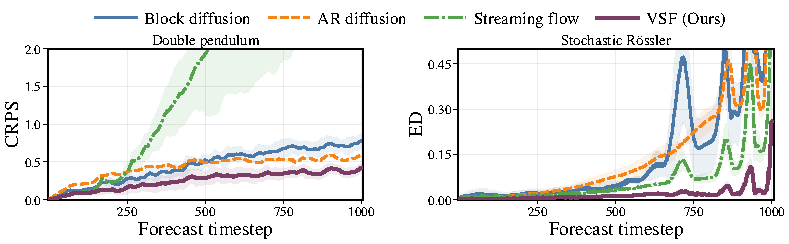
\includegraphics[width=\linewidth]{figures/rollout_error_plots/combined/rollout_errors_side_by_side.pdf}
  \vspace{-3em}
  \caption{VSF is less susceptible to error accumulation over long horizons
  because it conditions rollouts on variational latent code. Streaming
  Flow accumulates errors more easily because it relies entirely on previously
  predicted states. Left: continuous ranked probability score (CRPS) on
  deterministic double pendulum. Right: conditional mean error (CME) on
  partially observed R\"ossler. Additional deterministic and stochastic
  rollout results are in Appendix~\ref{sec:rollout-error-curves}.}
  \label{fig:main-rollout-error-curves}
\end{figure}


\section{Introduction}

% Forecasting complex dynamical systems requires predicting how a state evolves over long horizons from a finite observation history~\citep{zhang2025zero}. In fully observed deterministic systems, the history determines a single future, and the main challenge is to propagate the dynamics accurately as prediction errors accumulate over time. Under partial observability or stochastic dynamics, the same observed history may instead admit multiple futures, so the forecasting problem becomes distributional rather than point-valued~\citep{pfister2026stocbench}. This is particularly important when initially similar trajectories can evolve toward qualitatively different future regimes. A point forecast can then miss the distinct modes that define the predictive distribution. Probabilistic dynamics models have long been used in model-based control precisely because planning depends on the distribution of possible outcomes under a candidate action sequence~\citep{chua2018deep}. The same issue arises in modern learned world models, where predicted futures are used to evaluate and select candidate behaviors~\citep{zhou2025dinowm,maes2026leworldmodel}. Recent stochastic world models therefore explicitly model multimodal future evolution rather than relying on a single predicted endpoint~\citep{porcher2026flow}.\hans{why modeling stochasticity is important. give some concrete examples, what will happen if we dont model stochasticity}

Probabilistic forecasting is essential when small uncertainties in a dynamical system can grow into materially different futures. In fully observed deterministic systems, the future is unique, but error accumulation can compound over long rollouts~\citep{zhang2025zero}. Probabilistic forecasting mitigates this issue by averaging over an ensemble of samples. The need for distributional forecasting becomes fundamental under partial observability or stochastic forcing, where the same observed history can support multiple future trajectories~\citep{pfister2026stocbench}. For example, unresolved atmospheric processes and imperfect initial conditions can produce several plausible storm tracks, while uncertain contact and friction can cause a manipulated object to stick, slide, or topple. A point predictor optimized for average error may collapse these alternatives into an over-smoothed or physically invalid future. Recursively feeding such an average back into the model can amplify forecast errors and distort long-run statistics; using it for planning can obscure high-impact outcomes and lead to unsafe or unsuccessful actions~\citep{chua2018deep,porcher2026flow}. Probabilistic forecasting instead preserves distinct future modes and enables predictions and decisions that account for the range of plausible outcomes.

%%%%%%%%%%%%%%%%%%%%%%%%%%%%%%%%%%%%%%%%%%%%%%%%%%%%%%%%%%%%%%%%%%%%%%%%%%%%%%%%%%%%%%%%%%%%%%%%%%%%%%%%%%%%%%%%%%%%%%%%%%%%%%%%%%%%%%%%%%%%%%%%%%%%%%%%%%%%%%%%%%%%%%
\begin{figure}[t]
  \centering
  \includegraphics[
    width=\linewidth,
    trim={5bp 0bp 0bp 5bp},
    clip
  ]{figures/vsf_motivation.pdf}
  \vspace{-0.7cm}
  \caption{\textbf{SF vs. VSF.} (A) Fully observable deterministic dynamics yield a unique future, whereas partially observable stochastic dynamics admit multiple plausible futures. (B) VSF captures this stochasticity by generating multiple plausible trajectories, whereas SF produces a single prediction.}
  \label{fig:forecasting-settings}
  %\hans{Link in the comment}
  % Link: https://drive.google.com/file/d/1VlHFP2pe0Q471FzFswVsvX5lGRsEucYs/view?usp=sharing
\end{figure}

%%%%%%%%%%%%%%%%%%%%%%%%%%%%%%%%%%%%%%%%%%%%%%%%%%%%%%%%%%%%%%%%%%%%%%%%%%%%%%%%%%%%%%%%%%%%%%%%%%%%%%%%%%%%%%%%%%%%%%%%%%%%%%%%%%%%%%%%%%%%%%%%%%%%%%

% % \hans{mention why streaming flow, why this is an exciting problem, it looks like A+B style, efficiency}
% % \hans{improving stochaticity is natural}
% Flow matching has recently emerged as a promising approach for generative forecasting of complex dynamical systems~\citep{lim2026flow,porcher2026flow}. Standard flow models generate samples by evolving along an auxiliary flow-time coordinate. Streaming Flow Policy instead identifies the flow trajectory with the temporal action evolution itself, avoiding a separate generative trajectory over complete action sequences~\citep{jiang2025streaming}. Related physical-time formulations have since been explored for sequential prediction and world modeling~\citep{lim2026flow,liu2026odeworld}. These approaches learn how the state changes locally and construct the forecast by integrating these learned dynamics through physical time. However, when the observed initial state and history are fixed, a deterministic velocity field defines only a single rollout. Stochasticity can be introduced through perturbations of the initial state or history, but the resulting predictive distribution then depends on an externally chosen perturbation mechanism and its scale.

\hans{try to avoid saying we are doing flow matching because we don't use flow to model distribution}Flow matching provides a general mechanism for probabilistic forecasting by transporting a simple reference distribution into a conditional distribution over future trajectories~\citep{lipman2024flow,kollovieh2025tsflow}. A complete future can be treated as a high-dimensional sample, and a learned vector field transports noise toward this sample along an auxiliary flow coordinate. This coordinate measures progress from noise to data rather than the physical time of the predicted system, which can be computationally expensive for long horizons and online prediction. Another way to interpret the vector field is to align its integration coordinate with physical time~\citep{jiang2025streaming,liu2026odeworld}. The field then advances the observed state directly, and its intermediate solutions are successive forecast states rather than intermediate stages of a generative transport. This removes the separate noise-to-trajectory process and enables efficient forecasting. However, once the flow starts from an exact observed state instead of a random reference sample, the noise-free formulation considered here contains no source of randomness. For a fixed observation history, its deterministic physical-time velocity field therefore produces only one future trajectory.


\hans{updated} We address this limitation with \emph{Variational Streaming Flow} (VSF), which represents uncertainty over the physical-time dynamics. Given an observed history $\vx_{a:m}$, let $\vh=H(\vx_{a:m})$ denote its representation and let $s\in[0,1]$ denote normalized physical forecast time. Existing physical-time flow~\cite{jiang2025streaming} learns a deterministic velocity field $\vv_{\vtheta}(\vx,s,\vh)$, where $\vtheta$ denotes the model parameters. For a fixed history and initial state $\vx_m$, this field determines a single future evolution. VSF instead introduces a latent variable $\vz\sim p(\vz)$ that conditions the velocity field and indexes different possible dynamics. Starting from the observed state $\widehat{\vx}_0=\vx_m$, the forecast evolves as
%
\begin{tcolorbox}[
  colback=parchment,
  colframe=sandborder,
  boxrule=0.3pt,
  left=8pt,
  right=8pt,
  top=3pt,
  bottom=3pt
]
\begin{equation}
\frac{d\widehat{\vx}_s}{ds}
=
\vv_{\vtheta}\!\left(
    \widehat{\vx}_s,s,\vh,\vz
\right),
\qquad s\in[0,1].
\label{eq:intro_vsf}
\end{equation}
\end{tcolorbox}
% 
% \pan{this is more like Variational RNN than a flow model. I think some discussion may be needed somewhere.}
During training, an amortized variational posterior associates observed local transitions with latent codes, while prior regularization makes samples from the fixed prior usable at inference. A sample-based energy-score objective encourages different latent-conditioned velocities to represent the conditional variability in the observed dynamics~\citep{gneiting2007strictly,bouchacourt2016disco}. At inference, one latent variable is sampled for each forecast and shared throughout the rollout, selecting a common physical-time dynamics for that trajectory. Marginalizing the resulting trajectories over latent draws induces the predictive distribution. \hans{(Pan's suggestion: separate out us from flow matching)} VSF therefore does not construct this distribution by transporting reference noise through an auxiliary flow. Instead, the variational latent-variable model represents uncertainty over the dynamics, while the flow advances each sampled dynamics through physical time.





Our VSF formulation provides a flexible model for deterministic and probabilistic forecasting. When the observed history determines the future, the predictive distribution can concentrate around a single evolution. When several continuations are possible, the latent-conditioned dynamics can instead represent distinct modes of future evolution. We evaluate VSF on deterministic
and stochastic dynamical systems, including chaotic dynamics and settings with branching future trajectories. On deterministic R\"ossler and Lorenz, VSF achieves lower predictive error than autoregressive and diffusion-based forecasters, as well as Streaming Flow (SF)~\citep{jiang2025streaming}
and Chronos-2~\citep{ansari2025chronos}, variational RNN~\citep{salinas2020deepar}, while retaining near-streaming inference cost. On stochastic R\"ossler and Lorenz, VSF more accurately recovers the conditional distribution of long-horizon futures. We further use VSF as the predictor in Joint-Embedding Predictive Architecture (JEPA)-based world model to generate action-conditioned future trajectories \cite{maes2026leworldmodel}. Across the four robotics tasks, VSF improves goal-directed planning success by on average $7.34\%$ over the deterministic predictor used by the LeWM~\citealp{maes2026leworldmodel}, without requiring additional NFEs.  

Our main contributions are \hans{modify later}:
%
\begin{itemize}[leftmargin=*]
    \item We introduce \emph{Variational Streaming Flow} (VSF), extending SF to probabilistic forecasting by modeling a distribution over physical-time dynamics. VSF supports both deterministic and stochastic forecasting while retaining direct generation in physical time.

    \item We develop a variational learning objective for the latent-conditioned
    velocity field and combine it with a generalized energy-score objective over
    multiple latent samples. We characterize its population form and show that it
    is strictly proper for $\lambda=1/2$ and $0<\alpha<2$.

    \item We evaluate VSF on deterministic and stochastic dynamical systems and
    as the predictor in a world model. VSF improves long-horizon predictive
    accuracy and distributional fidelity over autoregressive, diffusion, and
    streaming-flow baselines, while its action-conditioned forecasts improve
    goal-directed planning and retain streaming-flow inference
    efficiency.
\end{itemize}




\begin{figure}[t]
  \centering
  \includegraphics[
    width=0.80\linewidth,
    trim={0bp 10bp 0bp 12bp},
    clip
  ]{figures/vsf_lewm.pdf}
  \vspace{-0.8em}
  \caption{
  % \small 
  % \textbf{Action-conditioned prediction in the LeWM latent space}
  \textbf{Stochastic world modeling} 
  We replace LeWM's deterministic AR predictor with an action-conditioned VSF predictor while keeping the JEPA encoder and CEM planner fixed. 
  % Given an initial observation $o_s$ and a goal observation $o_g$, the encoder $\mathcal{E}$ produces latent embeddings $\widehat{x}_s$ and $x_g$. We observe that trajectories in the learned JEPA latent space are smooth, motivating a continuous physical-time predictor. For each CEM candidate action sequence and latent draw $z^{(j)}$, VSF rolls out an action-conditioned latent trajectory to $\widehat{x}_T$. The terminal cost $\lVert\widehat{x}_T-x_g\rVert_2^2$ scores each candidate, and CEM iteratively updates the action distribution toward a low-cost plan.
  }
  \label{fig:world-model-predictor}
  % Link: https://drive.google.com/file/d/1VlHFP2pe0Q471FzFswVsvX5lGRsEucYs/view?usp=sharing
\end{figure}










\section{Method: Variational Streaming Flow}
\label{sec:method}
In this work, we consider sequential forecasting from an observed history $\vx_{a:m}=(\vx_a,\ldots,\vx_m)$, where $\vx_k\in\mathcal X\subseteq\R^d$ denotes the system state at physical time $k$. Our goal is to learn a conditional generative model over future
trajectories, that takes the form
%
\begin{equation}
    \widehat{\vx}_{m+1:T}
    \sim
    Q_{\vtheta}(\cdot\mid\vx_{a:m}),
    \label{eq:forecast_distribution}
\end{equation}
%
%
where $Q_{\vtheta}$ denotes the model's conditional distribution over future trajectories, parameterized by $\vtheta$. 
% When the system is fully observed and deterministic, the true conditional distribution concentrates on a single future. Under partial observability or stochastic dynamics, the same history may admit multiple continuations and the target is instead a non-degenerate conditional distribution. 
We first describe how SF formulates forecasting directly in physical time. We then introduce a latent-conditioned extension that represents a distribution over these physical-time dynamics.

\subsection{Motivation: Beyond Single-Trajectory Flows in Physical Time}
\label{sec:physical-time-flow}

Standard flow matching for sequential forecasting transports entire physical sequences from a reference distribution to the data distribution along an auxiliary flow time~\citep{some_ref}. Streaming Flow (SF), instead, uses observed states as sources and their subsequent states as targets, thereby aligning flow time with physical time~\citep{jiang2025streaming,lim2026flow}. We use this formulation to
learn the local physical-time evolution starting from observed states.

Consider a training window $\vx_{a:T}$ with forecast origin $m$, and let
$P:=T-m$ denote the number of future steps. We use
$s\in[0,1]$ as normalized physical forecast time. For
$k=0,\ldots,P-1$, define
\begin{equation}
    I_k
    :=
    \left[
        \frac{k}{P},
        \frac{k+1}{P}
    \right),
    \qquad
    \alpha_s:=Ps-k,
    \qquad
    s\in I_k.
    \label{eq:physical_time_interval}
\end{equation}
Adjacent observations define the piecewise-linear training path 
\begin{align}
    \vx_s
    &:=
    (1-\alpha_s)\vx_{m+k}
    +
    \alpha_s\vx_{m+k+1},
    \label{eq:physical_time_interpolation}\\
    \vu_s
    &:=
    \frac{d\vx_s}{ds}
    =
    P\left(\vx_{m+k+1}-\vx_{m+k}\right).
    \label{eq:physical_time_velocity}
\end{align}
Here, $\vu_s$ is the velocity of the interpolation with respect to normalized
forecast time. The linear interpolation defines the target 
path for training in the chosen state representation; it does not assume that the
unobserved physical motion between two sampled states is itself linear.
%
Let
\begin{equation}
    \vh:=H(\vx_{a:m})
    \label{eq:history_representation}
\end{equation}
denote a deterministic representation of the observed history. A physical-time flow learns a velocity field
$\vv_{\vtheta}(\vx,s,\vh)$ and generates a forecast by solving the
initial-value problem
%
\begin{equation}
    \frac{d\widehat{\vx}_s}{ds}
    =
    \vv_{\vtheta}(\widehat{\vx}_s,s,\vh),
    \qquad
    \text{with initial condition } \quad
    \widehat{\vx}_0=\vx_m.
    \label{eq:deterministic_streaming_flow}
\end{equation}
%
The history representation $\vh$ remains fixed over the forecast, while the generated state $\widehat{\vx}_s$ evolves through the learned dynamics. At the end of each interval $I_k$, the resulting state provides the next forecast frame. This formulation removes the need to construct each forecast through a separate generative-time trajectory. 

% It exposes a limitation for probabilistic forecasting. 
% Introducing uncertainty by perturbing $\vx_m$ can produce multiple rollouts, but then the predictive distribution depends on an inference-time perturbation of the observed state.




%%%%%%%%%%%%%%%%%%%%%%%%%%%%%%%%%
\subsection{\hans{updated}Variational Streaming Flow}
\label{sec:variational-streaming-flow}


A limitation of standard non-latent Streaming Flow (SF)~\citep{jiang2025streaming}
appears when multiple future trajectories share (almost) the same physical
state before bifurcating. The following result isolates the resulting
fidelity--sensitivity tradeoff; the complete construction and proof appear with
Proposition~\ref{prop_motivate} in the appendix.

\hans{notation needs to update. Should we change to continuous notation with tube idea}
\begin{vsfproposition}[Fidelity--sensitivity tradeoff for non-latent SF]
\label{prop:sf_tradeoff_summary}
Under the symmetric two-branch construction and regularity assumptions used
for Proposition~\ref{prop_motivate} in the appendix, consider standard SF
initialized by $X_0\sim\mathcal N(0,\sigma_0^2)$ and the population-optimal
marginal field identified there. Define the bifurcation-time fidelity error
$\varepsilon_\tau:=W_2(P_\tau^{\mathrm{SF}},P_\tau^{\mathrm{data}})$ and the
physical-state sensitivity along the symmetric separator $x(s)\equiv0$ by
$J_{\tau,t}^{\mathrm{SF}}:=\partial_x\Phi_{\tau,t}^{\mathrm{SF}}(0)$. For
every fixed $t>\tau$ with $m(t)>0$, and with $(k,m,\tau)$ fixed,
\begin{equation}
    \begin{gathered}
        \varepsilon_\tau=\sigma_0e^{-k\tau},
        \qquad
        J_{\tau,t}^{\mathrm{SF}}
        =
        \exp\!\left[
            -k(t-\tau)
            +
            \frac{m(t)^2e^{2k(t-\tau)}}{2\varepsilon_\tau^2}
        \right],
        \\
        \sigma_0\downarrow0
        \quad\Longleftrightarrow\quad
        \varepsilon_\tau\downarrow0
        \quad\Longrightarrow\quad
        J_{\tau,t}^{\mathrm{SF}}\to\infty.
    \end{gathered}
    \label{eq:bifurcation_tradeoff_summary}
\end{equation}
\end{vsfproposition}

Proposition~\ref{prop:sf_tradeoff_summary} makes the representational
bottleneck explicit: the physical state must remain close to the shared
trajectory while also encoding which branch to follow, so improving fidelity
makes branch selection increasingly sensitive to physical-state perturbations.
In contrast, the ideal latent construction following
\cref{prop:sf_tradeoff_summary} realizes both branches from the
exact shared state while, for each fixed latent branch code, retaining
sensitivity $e^{-k(t-\tau)}$. This motivates placing branch information in a
trajectory-level latent variable rather than in perturbations of the physical
state.

To model multiple local evolutions from the same observed history, VSF
augments the physical-time velocity field with a latent variable
\begin{equation}
    \vz\sim p(\vz)
    :=
    \mathcal N(\vz;\vzero,\mI_{d_z})
    \label{eq:latent_prior}
\end{equation}
drawn from a fixed prior. The latent variable is unobserved during training.
For each local training tuple $(\vu_s,\vx_s,s,\vh)$, we therefore introduce
the diagonal-Gaussian variational posterior
\begin{equation}
    q_{\vphi}(\vz\mid\vu_s,\vx_s,s,\vh)
    =
    \mathcal N\!\left(
        \vz;
        \vmu_{\vphi}(\vu_s,\vx_s,s,\vh),
        \operatorname{diag}\!\left(
            \vsigma_{\vphi}^2(\vu_s,\vx_s,s,\vh)
        \right)
    \right).
    \label{eq:vsf_variational_posterior}
\end{equation}
This construction follows variational latent-variable formulations of flow
matching~\citep{guo2025variational,eijkelboom2024variational}. Let
$p_{\vtheta}(\vu_s\mid\vx_s,s,\vh,\vz)$ denote the conditional velocity
likelihood. Marginalizing the latent variable gives
\begin{equation}
    p_{\vtheta}(\vu_s\mid\vx_s,s,\vh)
    :=
    \int
    p_{\vtheta}(\vu_s\mid\vx_s,s,\vh,\vz)
    p(\vz)\,d\vz.
    \label{eq:vsf_velocity_evidence}
\end{equation}
From \cref{prop:velocity_elbo}, the corresponding conditional evidence lower bound (ELBO) is
\begin{align}
    \log p_{\vtheta}(\vu_s\mid\vx_s,s,\vh)
    \geq{}&
    \E_{q_{\vphi}(\vz\mid\vu_s,\vx_s,s,\vh)}
    \!\left[
        \log p_{\vtheta}(\vu_s\mid\vx_s,s,\vh,\vz)
    \right]
    \notag\\
    &-
    \KL\!\left(
        q_{\vphi}(\vz\mid\vu_s,\vx_s,s,\vh)
        \,\Vert\,
        p(\vz)
    \right)
    =:
    \mathcal E_{\vtheta,\vphi}(\vu_s,\vx_s,s,\vh).
    \label{eq:vsf_elbo}
\end{align}
The expected log-likelihood fits the observed local velocity using latent
codes inferred from that transition, while the KL term regularizes those
codes toward the prior used at inference.

At inference, we draw one $\vz\sim p(\vz)$ for each forecast and keep it
fixed throughout the rollout. Starting from $\widehat{\vx}_0=\vx_m$, the
latent-conditioned state evolves according to
\begin{equation}
    \frac{d\widehat{\vx}_s}{ds}
    =
    \vv_{\vtheta}\!\left(
        \widehat{\vx}_s,s,\vh,\vz
    \right),
    \qquad s\in[0,1].
    \label{eq:vsf_dynamics}
\end{equation}
Thus, different latent draws can index different velocity fields without
perturbing the observed initial state, and the shared latent couples the
generated evolution across physical time. For fixed $(\vx_{a:m},\vz)$,
Eq.~\ref{eq:vsf_dynamics} defines one trajectory; marginalizing over the
prior induces the conditional forecast distribution
\begin{equation}
    Q_{\vtheta}(\cdot\mid\vx_{a:m})
    :=
    \operatorname{Law}_{\vz\sim p(\vz)}
    \left[
        \widehat{\vx}_{m+1:T}(\vz)
    \right].
    \label{Eq:vsf_predictive_distribution}
\end{equation}
% This parameterization permits the predictive law to concentrate when the
% future is effectively determined by the history, or to represent latent-dependent alternatives when the observed dynamics support them.

\subsection{\hans{updated}Distributional Learning with a Generalized Energy Reconstruction}
\label{sec:vsf-learning}

A conventional realization of the likelihood in Eq.~\ref{eq:vsf_elbo} is a
fixed-variance Gaussian centered at the predicted velocity.
Taking expectations over
$\vz$, the negative reconstruction
term is, up to an additive constant,
\begin{equation}
    -\E_{\vz}
    \!\left[
        \log p_{\vtheta}(\vu_s\mid\vx_s,s,\vh,\vz)
    \right]
    =
    \frac{1}{2\sigma_u^2}
    \E_{\vz}
    \!\left[
        \left\|
            \vv_{\vtheta}(\vx_s,s,\vh,\vz)-\vu_s
        \right\|_2^2
    \right]
    +\mathrm{const},
    \label{eq:vsf_variational_mse}
\end{equation}
The standard Gaussian ELBO reduces to a variational MSE
reconstruction together with prior regularization.
To characterize the MSE solution, let
$p_{\mathrm{data}}(\cdot\mid\vx_s,s,\vh)$ denote the true conditional
distribution of the velocity target. Here $\vu$ denotes a generic possible
value of the observed target $\vu_s$. For the population analysis, sample
\begin{equation*}
    \vu\sim p_{\mathrm{data}}(\cdot\mid\vx_s,s,\vh),
    \qquad
    \vz\sim q_{\vphi}(\cdot\mid\vu,\vx_s,s,\vh).
\end{equation*}
For a fixed $q_{\vphi}$ and an unrestricted decoder, minimizing population
MSE gives
\begin{equation}
    \vv_{\mathrm{MSE}}^\star(\vx_s,s,\vh,\vz)
    =
    \E\!\left[
        \vu\mid\vx_s,s,\vh,\vz
    \right].
    \label{eq:vsf_mse_conditional_mean}
\end{equation}
\hans{Please have a look at this part! Thank you}When $\vz$ identifies a branch, this conditional mean is branch-specific.
In practice, however, variational training can produce overlapping
branch-specific posteriors and, in the limiting case, posterior
collapse. Whenever multiple branches remain possible at the same
$(\vx_s,s,\vh,\vz)$, Eq.~\ref{eq:vsf_mse_conditional_mean} averages their
unresolved velocity ambiguity. Limited latent dimension and encoder capacity
can exacerbate this effect. This averaging motivates a reconstruction loss
that evaluates the posterior predictions jointly, accounting for both their
agreement with the target and their spread. We therefore draw

\begin{equation}
    \vz^{(i)}
    \sim
    q_{\vphi}(\vz\mid\vu_s,\vx_s,s,\vh),
    \qquad
    i=1,\ldots,M,
    \label{eq:posterior_latent_samples}
\end{equation}
and obtain the corresponding velocity predictions
\(
    \widehat{\vu}_s^{(i)}
    :=
    \vv_{\vtheta}
    \left(
        \vx_s,
        s,
        \vh,
        \vz^{(i)}
    \right).
    \label{eq:posterior_velocity_samples}
\)
We then use a generalized energy reconstruction with the same attraction and
self-dissimilarity terms as the energy score,
\begin{equation}
    \mathcal L_{\mathrm{ES}}
    :=
    \frac{1}{M}
    \sum_{i=1}^{M}
    \left\|
        \widehat{\vu}_s^{(i)}-\vu_s
    \right\|_2^\alpha
    -
    \frac{1}{2M^2}
    \sum_{i,j=1}^{M}
    \left\|
        \widehat{\vu}_s^{(i)}
        -
        \widehat{\vu}_s^{(j)}
    \right\|_2^\alpha,
    \qquad
    0<\alpha<2.
    \label{eq:vsf_energy_score}
\end{equation}
The first term attracts posterior-generated velocities toward the observed
target. The second  term preserves separation between generated samples \citep{bouchacourt2016disco}. In practice, this yields a less contractive training
signal when branch information is not perfectly separated in latent space. For $\alpha=1$, Eq.~\ref{eq:vsf_energy_score} has the standard energy-score
form and reduces to the CRPS. 
% When the forecast law is
% specified independently of the realized target and both laws have finite
% $\alpha$-moments, the corresponding population score is strictly proper for
% $0<\alpha<2$~\citep{gneiting2007strictly};
% Appendix~\ref{sec:crps_mae_propriety} states the result and its assumptions.

We retain the ELBO's prior-matching
regularizer and optimize the KL-regularized distributional objective. The complete batched training procedure is summarized in
\cref{alg:vsf-training}.
%
\begin{tcolorbox}[
  colback=parchment,
  colframe=sandborder,
  boxrule=0.3pt,
  left=8pt,
  right=8pt,
  top=3pt,
  bottom=3pt
]
\begin{equation}
    \mathcal L_{\mathrm{VSF}}
    =
    \mathcal L_{\mathrm{ES}}
    +
    \beta_{\mathrm{KL}}
    \KL\!\left(
        q_{\vphi}(\vz\mid\vu_s,\vx_s,s,\vh)
        \,\Vert\,
        p(\vz)
    \right).
    \label{eq:vsf_training_objective}
\end{equation}
\end{tcolorbox}
%
% Here $\beta_{\mathrm{KL}}$ controls the trade-off between retaining
% target-specific information in $\vz$ and matching the inference prior. 
% The posterior is used only during training; forecasts use $\vz\sim p(\vz)$ as in
% Eq.~\ref{eq:latent_prior}. 
%


Let $S_\alpha(\vu)$ denote the
expectation-level counterpart of the generalized energy reconstruction in
Eq.~\ref{eq:vsf_energy_score}. Also draw
$\widetilde{\vz}\sim p(\vz)$, set
$\widetilde{\vu}:=\vv_{\vtheta}(\vx_s,s,\vh,\widetilde{\vz})$, and let
$D_\alpha(\widetilde{\vu},\vu)$ denote the generalized energy distance
between this prior-predictive velocity and the true conditional velocity.

\begin{vsfproposition}[Prior-predictive energy-distance control]
\label{prop:energy_control}
Assume $0<\alpha<2$ and finite $\alpha$-moments. \(\overline q_{\vphi}(\vz\mid\vx_s,s,\vh)
    :=
    \E_{\vu\sim p_{\mathrm{data}}}
    \!\left[
        q_{\vphi}(\vz\mid\vu,\vx_s,s,\vh)
    \right]\). If
$\overline q_{\vphi}(\vz\mid\vx_s,s,\vh)=p(\vz)$ almost everywhere,
then
\begin{equation*}
  \frac12D_\alpha(\widetilde{\vu},\vu)
  \leq
  \E_{\vu\sim p_{\mathrm{data}}(\cdot\mid\vx_s,s,\vh)}
  \!\left[S_\alpha(\vu)\right].
\end{equation*}
\end{vsfproposition}
% \Cref{prop:energy_control} shows the expected energy reconstruction upper-bounds half the energy distance between the decoded aggregate posterior and the true conditional velocity. Thus, reducing the reconstruction objective controls a distribution-level discrepancy, rather than only an error in the conditional mean.

% Unlike the pointwise Gaussian/MSE reconstruction used in a conventional
% ELBO, Eq.~\ref{eq:vsf_energy_score} defines a distributional reconstruction
% over the decoded ensemble. \Cref{prop:energy_control} formalizes this
% distinction: the expected reconstruction upper-bounds half the energy distance
% between the decoded aggregate-posterior distribution and the true conditional
% velocity distribution. Thus, for $0<\alpha<2$, a small reconstruction loss
% guarantees a small distributional discrepancy rather than only a small
% conditional-mean error.

Unlike the pointwise Gaussian reconstruction used in Eq.~\ref{eq:vsf_variational_mse}, Eq.~\ref{eq:vsf_energy_score} defines a distributional reconstruction
over the decoded ensemble. \Cref{prop:energy_control} shows the expected energy reconstruction upper-bounds half the energy distance between the decoded aggregate posterior and the true conditional velocity. Thus, reducing the reconstruction objective controls a distribution-level discrepancy.
















% %%%%%%%%%%%%%%%%%%%%%%%%%%%%%%%%
% \subsection{\hans{legacy}Variational Streaming Flow}
% \label{sec:variational-streaming-flow}

% To overcome this limitation of SF, we introduce
% VSF. VSF extends deterministic
% physical-time forecasting to a probabilistic model over future trajectories by conditioning the velocity field on a latent variable. Different latent draws can therefore induce different future evolutions from the same observed history. Let
% \begin{equation}
%     \vz\sim p(\vz)
%     :=
%     \mathcal N(\vz;\vzero,\mI_{d_z})
%     \label{eq:latent_prior}
% \end{equation}
% be a latent vector drawn from a fixed prior. VSF conditions the velocity field on this latent variable. 
% %
% Starting from the observed state $\widehat{\vx}_0=\vx_m$, a latent-conditioned forecast evolves according to
% %
% \begin{equation}
%     \frac{d\widehat{\vx}_s}{ds}
%     =
%     \vv_{\vtheta}
%     \left(
%         \widehat{\vx}_s,
%         s,
%         \vh,
%         \vz
%     \right),
%     \qquad
%     s\in[0,1].
%     \label{eq:vsf_dynamics}
% \end{equation}
% %
% Different latent draws can therefore induce different velocity fields from the same observed history without perturbing the initial state. We draw one latent vector for each forecast and keep it fixed throughout the rollout. The shared latent \pan{vector} couples the generated evolution across physical time.

% For fixed $(\vx_{a:m},\vz)$, \cref{eq:vsf_dynamics} defines one forecast
% trajectory. Marginalizing over the latent prior induces the conditional
% forecast distribution
% \begin{equation}
%     Q_{\vtheta}(\cdot\mid\vx_{a:m})
%     :=
%     \operatorname{Law}_{\vz\sim p(\vz)}
%     \left[
%         \widehat{\vx}_{m+1:T}(\vz)
%     \right].
%     \label{Eq:vsf_predictive_distribution}
% \end{equation}
% This gives the same formulation two different behaviors. If the observed
% history determines a unique future, the learned predictive distribution can
% concentrate around that evolution. If several continuations are supported by
% the data, different latent-conditioned velocity fields can represent distinct
% future trajectories. \pan{why for the previous two statements? Any proof/reference for this? The statement may need to be tuned down.}

% \subsection{Learning a Distribution over Local Dynamics}
% \label{sec:vsf-learning}

% The latent variable in Eq.~\ref{eq:vsf_dynamics} is unobserved. During
% training, we therefore introduce a variational posterior that infers latent
% dynamics from an observed local transition. For the training tuple
% $(\vu_s,\vx_s,s,\vh)$, we use
% \begin{equation}
%     q_{\vphi}(\vz\mid\vu_s,\vx_s,s,\vh)
%     =
%     \mathcal N\!\left(
%         \vz;
%         \vmu_{\vphi}(\vu_s,\vx_s,s,\vh),
%         \operatorname{diag}
%         \left(
%             \vsigma_{\vphi}^2(\vu_s,\vx_s,s,\vh)
%         \right)
%     \right).
%     \label{eq:vsf_variational_posterior}
% \end{equation}
% This follows the variational latent-variable construction used in recent
% flow matching models~\citep{guo2025variational,eijkelboom2024variational}.
% For a fixed-variance Gaussian velocity likelihood, the corresponding
% reconstruction and KL terms form a variational lower bound on the conditional
% velocity evidence; we give the derivation in
% Appendix~\ref{sec:clean_velocity_elbo}.

% Our goal, however, is not only to reconstruct one observed velocity. We want
% the latent-conditioned model to represent its conditional distribution. We
% therefore draw
% \begin{equation}
%     \vz^{(i)}
%     \sim
%     q_{\vphi}(\vz\mid\vu_s,\vx_s,s,\vh),
%     \qquad
%     i=1,\ldots,M,
%     \label{eq:posterior_latent_samples}
% \end{equation}
% and obtain the corresponding velocity predictions
% \begin{equation}
%     \widehat{\vu}_s^{(i)}
%     :=
%     \vv_{\vtheta}
%     \left(
%         \vx_s,
%         s,
%         \vh,
%         \vz^{(i)}
%     \right).
%     \label{eq:posterior_velocity_samples}
% \end{equation}
% We train these samples with the generalized energy score \pan{how is the above variational lower bound connected to the generalized energy score? My feeling is that the loss adopted here is just pure heuristic.}
% \begin{equation}
%     \mathcal L_{\mathrm{ES}}
%     :=
%     \frac{1}{M}
%     \sum_{i=1}^{M}
%     \left\|
%         \widehat{\vu}_s^{(i)}-\vu_s
%     \right\|_2^\alpha
%     -
%     \frac{1}{2M^2}
%     \sum_{i,j=1}^{M}
%     \left\|
%         \widehat{\vu}_s^{(i)}
%         -
%         \widehat{\vu}_s^{(j)}
%     \right\|_2^\alpha,
%     \qquad
%     0<\alpha<2.
%     \label{eq:vsf_energy_score}
% \end{equation}
% The first term encourages agreement with the observed local dynamics. The
% second compares latent-conditioned predictions with one another and prevents
% the objective from rewarding a collapsed distribution when the data support
% multiple velocities  \pan{It is unclear to me why a flow model needs the second term to keep diversity. All these read hueristic.}. For $\alpha=1$, this reduces to the energy score, and to
% the CRPS in the scalar case~\citep{gneiting2007strictly}. Related
% sample-based distributional objectives have been used to learn diverse
% predictive distributions without an explicit density
% parameterization~\citep{bouchacourt2016disco}. In practice we found setting $\alpha$ close to $2$ gives better performance and set $\alpha=1.999$ for all experiments.
% \hans{should first write the conventional vae first}
% The variational posterior is available only during training. At inference,
% the latent must instead be drawn from the prior in
% Eq.~\ref{eq:latent_prior}. We therefore regularize the posterior toward this
% prior and optimize \pan{similar here, if this is derived from variational bound, how does the energy score come from?}
% %
% \begin{tcolorbox}[
%   colback=parchment,
%   colframe=sandborder,
%   boxrule=0.3pt,
%   left=8pt,
%   right=8pt,
%   top=3pt,
%   bottom=3pt
% ]
% \begin{equation}
%     \mathcal L_{\mathrm{VSF}}
%     =
%     \mathcal L_{\mathrm{ES}}
%     +
%     \beta
%     \KL\!\left(
%         q_{\vphi}(\vz\mid\vu_s,\vx_s,s,\vh)
%         \,\Vert\,
%         p(\vz)
%     \right).
%     \label{eq:vsf_training_objective}
% \end{equation}
% \end{tcolorbox}
% %
% The energy-score term learns a distribution of plausible local velocities, while the KL term aligns the training-time latent posterior with the inference-time prior. The population form of
% Eq.~\ref{eq:vsf_energy_score} provides a useful interpretation of this
% objective. For a target-independent forecast law with finite $\alpha$-moments, the score with pairwise coefficient $1/2$ is strictly proper
% for $0<\alpha<2$~\citep{gneiting2007strictly}. Its population optimum therefore recovers the conditional velocity distribution \pan{proof or proposition? If you have proof, directly say we may show that xxx \ref xxx}. In the deterministic case, this distribution is a point mass; in the stochastic case, the same objective can retain nonzero variability and multimodality. We prove this result in Appendix~\ref{sec:crps_mae_propriety}.


\subsection{Forecasting and Action Conditioning}
\label{sec:vsf-inference}

We now describe how VSF generates forecast ensembles at inference and extends to action-conditioned prediction for world models. At inference, only the learned velocity field and latent prior are required. Given an observed history $\vx_{a:m}$, we first compute
$\vh=H(\vx_{a:m})$. For each ensemble member $j=1,\ldots,M$, we independently draw
%
\begin{equation}
    \vz^{(j)}\sim p(\vz)
    \label{eq:vsf_inference_latents}
\end{equation}
%
once and initialize $\widehat{\vx}_m^{(j)}=\vx_m$. Each latent is then kept fixed for the entire forecast.

For $k=0,\ldots,P-1$, the model evolves ensemble member $j$ over
$I_k$ according to
\begin{equation}
    \frac{d\widehat{\vx}_s^{(j)}}{ds}
    =
    \vv_{\vtheta}
    \left(
        \widehat{\vx}_s^{(j)},
        s,
        \vh,
        \vz^{(j)}
    \right),
    \qquad s\in I_k,
    \label{eq:vsf_inference_ode}
\end{equation}
and emits the next forecast state at the end of the interval. 
The history $\vh$ is held fixed only within each rollout
window and is refreshed with generated states between windows. The
corresponding single-trajectory rollout is summarized in
\cref{alg:vsf-inference}. Within a window, temporal dependence is propagated
through the evolving state $\widehat{\vx}_s$. The
ensemble members are conditionally independent given the observed history and
can be generated in parallel. Equivalently, the continuous trajectory satisfies
\begin{equation}
    \widehat{\vx}_s^{(j)}
    =
    \vx_m
    +
    \int_0^s
    \vv_{\vtheta}
    \left(
        \widehat{\vx}_\tau^{(j)},
        \tau,
        \vh,
        \vz^{(j)}
    \right)
    \,d\tau,
    \qquad s\in[0,1].
    \label{eq:vsf_integral_solution}
\end{equation}
In practice, this integral is evaluated using a numerical ODE solver.

\paragraph{Action-conditioned forecasting.}
For controlled dynamics, let $\va_k$ denote the action applied during the
transition from $\vx_k$ to $\vx_{k+1}$. We supply the aligned action directly
to the velocity field,
\begin{equation}
    \frac{d\widehat{\vx}_s}{ds}
    =
    \vv_{\vtheta}
    \left(
        \widehat{\vx}_s,
        s,
        \vh,
        \va_{m+k},
        \vz
    \right),
    \qquad
    s\in I_k.
    \label{eq:vsf_action_conditioned_dynamics}
\end{equation}
The same action is included in the variational posterior during training.
The autonomous model is recovered by omitting this argument.



Following goal-directed planning with world models \citep{zhou2025dinowm,maes2026leworldmodel}, we use the action-conditioned VSF to evaluate candidate action sequences. Let $\va_{m:T-1}^{(i)}$ denote candidate $i$ and $\vx_g$ the goal. For each candidate, VSF predicts the resulting trajectory and assigns the terminal cost $\widehat J_{\vtheta}^{(i)} := d_g\left(\widehat{\vx}_T^{(i)},\vx_g\right)$, where $\widehat{\vx}_T^{(i)}$ is the predicted terminal state by VSF.

% We use this action-conditioned model as the predictor in a world model to
% generate future trajectories under candidate action sequences. Following
% goal-directed planning with learned world models
% ~\citep{zhou2025dinowm,maes2026leworldmodel}, let
% $\va_{m:T-1}^{(i)}$ denote candidate $i$ and let $\vx_g$ denote the goal.
% For each candidate, VSF generates $M$ imagined trajectories and estimates its
% terminal cost by
% \begin{equation}
%     \widehat J_{\vtheta}^{(i)}
%     :=
%     \frac{1}{M}
%     \sum_{j=1}^{M}
%     d_g\!\left(
%         \widehat{\vx}_T^{(i,j)},
%         \vx_g
%     \right).
%     \label{eq:vsf_world_model_cost}
% \end{equation}
The planner uses these expected imagined costs to compare candidate action
sequences. We use the cross-entropy method (CEM)~\citep{rubinstein1999cross}, a gradient-free optimizer that iteratively samples candidate action sequences, evaluates their predicted performance, and updates the sampling distribution toward the lowest-cost samples. This extends the usual
single-prediction planning objective to a distribution over imagined futures,
as in probabilistic model-based control~\citep{chua2018deep}.

If the action-conditioned terminal distribution produced by the world model matches the environment terminal distribution for every candidate
action sequence, then their expected terminal costs agree and the ideal
model-based and environment planning objectives have the same minimizers. 
% We provide this planning-consistency statement in \cref{prop:world_model_planning_consistency}.

%\section{Theoretical Results}
%\label{sec:theory}


\section{Experimental Results}
\label{sec:results}

In this section, we evaluate VSF as a probabilistic forecasting model for fully observed dynamical systems (\Cref{sec:exp-deterministic}) and partially observed dynamical systems (\Cref{sec:exp-stochatic}), verifying its effectiveness as a predictor in world-model planning (\Cref{sec:exp-world-model}) .

\paragraph{Baselines.}
For the dynamical-system forecasting experiments, we compare VSF with seven
baselines: (1) Block diffusion, a conditional diffusion model that generates
the forecast horizon jointly; (2) AR diffusion, an autoregressive diffusion
model that generates one future state at a time; (3) DeepAR
~\citep{salinas2020deepar}, an autoregressive recurrent probabilistic
forecaster; (4) SF~\citep{jiang2025streaming}, a deterministic
physical-time flow; (5) SF (perturbation), which introduces
forecast diversity through Gaussian perturbations of the initial state; (6)
Chronos-2~\citep{ansari2025chronos}, a pretrained universal time-series
forecaster; and (7) Chronos-2 (calibrated), which applies post-hoc calibration
to the Chronos-2 predictions.

\begin{table}[t]
\centering
\caption{Long-horizon forecasting on deterministic and stochastic dynamical systems over a 1,000-step rollout. Bold: best. Runtime is averaged across tasks.}
\label{tab:forecasting_results}
\begingroup
\normalsize
\setlength{\tabcolsep}{2pt}

% ==================== Deterministic ====================
\resizebox{\linewidth}{!}{%
\begin{tabular}{@{}l*{3}{>{\columncolor{resultDPBg}}c}*{3}{>{\columncolor{resultRosslerBg}}c}*{3}{>{\columncolor{resultLorenzBg}}c}>{}r@{}}
\toprule
% \rowcolor{gray!20}
\multicolumn{11}{c}{\cellcolor{gray!10}{Deterministic dynamics}}\\
& \multicolumn{3}{c}{\cellcolor{resultDPBg}{Double pendulum}}
& \multicolumn{3}{c}{\cellcolor{resultRosslerBg}{R\"ossler}}
& \multicolumn{3}{c}{\cellcolor{resultLorenzBg}{Lorenz}}
& \\
\cmidrule(lr){2-4}\cmidrule(lr){5-7}\cmidrule(lr){8-10}
Model
& CRPS $\downarrow$ & RMSE $\downarrow$ & MAE $\downarrow$
& CRPS $\downarrow$ & RMSE $\downarrow$ & MAE $\downarrow$
& CRPS $\downarrow$ & RMSE $\downarrow$ & MAE $\downarrow$
& Runtime (s) \\
\midrule
Block diffusion
& \resultpm{0.46}{0.07} & \resultpm{0.91}{0.14} & \resultpm{0.47}{0.07}
& \resultpm{0.29}{0.13} & \resultpm{0.54}{0.26} & \resultpm{0.29}{0.13}
& \resultpm{0.31}{0.12} & \resultpm{0.42}{0.18} & \resultpm{0.33}{0.12}
& 30.2 \\

AR diffusion
& \resultpm{0.43}{0.00} & \resultpm{0.96}{0.01} & \resultpm{0.59}{0.01}
& \resultpm{0.35}{0.06} & \resultpm{1.00}{0.13} & \resultpm{0.53}{0.08}
& \resultpm{0.86}{0.04} & \resultpm{1.96}{0.06} & \resultpm{1.50}{0.06}
& 78.2 \\

DeepAR
& \resultpm{0.58}{0.00} & \resultpm{1.07}{0.00} & \resultpm{0.68}{0.00}
& \resultpm{0.17}{0.04} & \resultpm{0.54}{0.05} & \resultpm{0.21}{0.05}
& \resultpm{10.30}{0.22} & \resultpm{12.42}{0.13} & \resultpm{10.88}{0.13}
& 3.9 \\

SF
& \resultpm{2.12}{0.87} & \resultpm{9.18}{5.17} & \resultpm{2.12}{0.87}
& \resultpm{0.16}{0.07} & \resultpm{0.34}{0.18} & \resultpm{0.16}{0.07}
& \resultpm{1.42}{0.14} & \resultpm{2.75}{0.31} & \resultpm{1.42}{0.14}
& 6.4 \\

SF (perturb.)
& \resultpm{1.83}{0.86} & \resultpm{8.38}{5.18} & \resultpm{1.96}{0.89}
& \resultpm{0.11}{0.05} & \resultpm{0.34}{0.18} & \resultpm{0.16}{0.07}
& \resultpm{1.39}{0.14} & \resultpm{2.75}{0.31} & \resultpm{1.42}{0.14}
& 6.4 \\

Chronos-2
& \resultpm{0.78}{0.00} & \resultpm{1.50}{0.02} & \resultpm{0.96}{0.01}
& \resultpm{1.98}{0.00} & \resultpm{4.11}{0.02} & \resultpm{2.62}{0.01}
& \resultpm{13.50}{0.06} & \resultpm{28.19}{1.14} & \resultpm{25.22}{0.85}
& 0.8 \\

Chronos-2 (calib.)
& \resultpm{0.62}{0.00} & \resultpm{1.16}{0.00} & \resultpm{0.74}{0.00}
& \resultpm{1.91}{0.00} & \resultpm{3.91}{0.02} & \resultpm{2.52}{0.01}
& \resultpm{2.39}{0.02} & \resultpm{6.01}{0.27} & \resultpm{4.54}{0.27}
& 0.4 \\

% \midrule
VSF
& \fullbestresultpm{0.25}{0.07} & \fullbestresultpm{0.71}{0.11} & \fullbestresultpm{0.33}{0.08}
& \fullbestresultpm{0.03}{0.00} & \fullbestresultpm{0.13}{0.01} & \fullbestresultpm{0.05}{0.00}
& \fullbestresultpm{0.16}{0.02} & \fullbestresultpm{0.25}{0.02} & \fullbestresultpm{0.19}{0.01}
& 7.2 \\
\bottomrule
\end{tabular}%
}

\vspace{-1.3pt}

% ===================== Stochastic =====================
\resizebox{\linewidth}{!}{%
\begin{tabular}{@{}l*{4}{>{\columncolor{resultRosslerBg}}c}*{4}{>{\columncolor{resultLorenzBg}}c}>{}r@{}}
\toprule
% \rowcolor{gray!20}
\multicolumn{10}{c}{\cellcolor{gray!10}{Stochastic dynamics}}\\
% \midrule
& \multicolumn{4}{c}{\cellcolor{resultRosslerBg}{R\"ossler}}
& \multicolumn{4}{c}{\cellcolor{resultLorenzBg}{Lorenz}}
& \\
\cmidrule(lr){2-5}\cmidrule(lr){6-9}
Model
& CME $\downarrow$ & CSE $\downarrow$ & $W_1$ $\downarrow$ & ED $\downarrow$
& CME $\downarrow$ & CSE $\downarrow$ & $W_1$ $\downarrow$ & ED $\downarrow$
& Runtime (s) \\
\midrule
Block diffusion
& \resultpm{0.16}{0.02} & \resultpm{0.72}{0.08} & \resultpm{8.88}{1.05} & \resultpm{12.67}{1.71}
& \resultpm{0.20}{0.01} & \resultpm{0.93}{0.01} & \resultpm{19.88}{0.28} & \resultpm{13.73}{0.45}
& 21.8 \\

AR diffusion
& \resultpm{0.20}{0.03} & \resultpm{4.63}{0.40} & \resultpm{16.21}{1.12} & \resultpm{11.46}{2.06}
& \resultpm{0.22}{0.05} & \resultpm{0.95}{0.14} & \resultpm{25.64}{3.10} & \resultpm{5.60}{1.54}
& 42.4 \\

DeepAR
& \resultpm{0.20}{0.02} & \resultpm{0.61}{0.02} & \resultpm{11.81}{0.80} & \resultpm{15.62}{1.57}
& \resultpm{2.14}{0.49} & \resultpm{2.61}{0.27} & \resultpm{131.84}{15.99} & \resultpm{138.30}{45.71}
& 1.2 \\

SF
& \resultpm{0.06}{0.02} & \resultpm{1.00}{0.00} & \resultpm{4.53}{0.67} & \resultpm{5.00}{1.34}
& \resultpm{1.04}{0.56} & \resultpm{1.00}{0.00} & \resultpm{58.12}{24.23} & \resultpm{89.84}{48.45}
& 7.5 \\

SF (perturb.)
& \resultpm{0.06}{0.02} & \resultpm{1.12}{0.23} & \resultpm{4.92}{0.84} & \resultpm{2.28}{0.82}
& \resultpm{0.68}{0.33} & \resultpm{1.33}{0.75} & \resultpm{53.62}{25.69} & \resultpm{35.78}{19.55}
& 6.6 \\

Chronos-2
& \resultpm{1.28}{0.06} & \resultpm{47.87}{1.63} & \resultpm{90.54}{3.86} & \resultpm{94.84}{0.79}
& \resultpm{6.84}{0.17} & \resultpm{37.49}{1.66} & \resultpm{411.32}{9.43} & \resultpm{342.98}{1.87}
& 0.3 \\

Chronos-2 (calib.)
& \resultpm{1.20}{0.06} & \resultpm{61.83}{2.09} & \resultpm{101.69}{4.61} & \resultpm{93.23}{0.20}
& \resultpm{1.44}{0.06} & \resultpm{10.53}{0.49} & \resultpm{111.81}{3.11} & \resultpm{64.97}{0.79}
& 0.1 \\

% \midrule
VSF
& \fullbestresultpm{0.04}{0.01} & \fullbestresultpm{0.36}{0.14} & \fullbestresultpm{2.62}{0.38} & \fullbestresultpm{1.28}{0.42}
& \fullbestresultpm{0.19}{0.03} & \fullbestresultpm{0.50}{0.21} & \fullbestresultpm{15.95}{5.64} & \fullbestresultpm{5.19}{0.93}
& 6.7 \\
\bottomrule
\end{tabular}%
}

\endgroup
\end{table}


\begin{figure}[t]
  \centering
  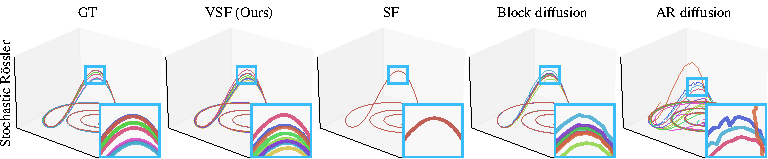
\includegraphics[width=0.88\linewidth]{figures/zoom_stochastic_rossler.pdf}
  \caption{Qualitative results on the stochastic R\"ossler system. We sampled $10$ trajectories from each method. VSF preserves the geometry of the GT dynamics while capturing plausible trajectory variability. Block diffusion produces less diverse trajectories, whereas AR diffusion is prone to drift.}
  \label{fig:qualitative-stochastic-rossler}
  \label{fig:qualitative-stochastic}
\end{figure}


\subsection{Deterministic Forecasting} \label{sec:exp-deterministic}

We evaluate fully observed deterministic forecasting on the Double-pendulum,
R\"ossler, and Lorenz systems using 1,000-step rollouts. We report CRPS for the
forecast ensemble and RMSE and MAE for its mean; detailed definitions are
provided in Appendix~\ref{sec:metrics}.

\textbf{VSF produces accurate forecasts with samples concentrated around the ground-truth trajectory.} As shown in Table~\ref{tab:forecasting_results}, VSF achieves the lowest CRPS, RMSE, and MAE across all three systems, while offering
up to a sevenfold speedup over AR diffusion. The qualitative forecasts in
Figures~\ref{fig:main-chaotic-double-pendulum}
further shows that its sampled
trajectories remain close to the reference dynamics throughout the rollout;
the other deterministic systems are shown in Appendix
Figure~\ref{fig:qualitative-deterministic}.
Chronos-2 is substantially less accurate across all our experiments due to our short forecasting context of only 10 time
steps. This interpretation is consistent with the findings of
\citet{zhang2025zero}, which use 512 context points in their main experiments
on chaotic systems and report improved zero-shot forecasting performance
for Chronos as the context length increases.


\textbf{Variational latent dynamics mitigate long-horizon drift caused by
error accumulation.} 
This effect is most apparent in the chaotic double-pendulum example in Figure~\ref{fig:main-chaotic-double-pendulum}. Although injecting noise into SF can partially mitigate drift caused by accumulated rollout errors, its forecasts still progressively deviate from the reference trajectory. In contrast, VSF combines the previous-frame representation with the latent variable $\vz$ through a weighted sum at the network bottleneck (see Appendix Experimental Details). By moderating the direct contribution of the previous-frame representation, this fusion can help limit error propagation, consistent with the more stable long-horizon rollouts observed for VSF \hans{this is related to the ablations study on how we fuse the latent code}.

\subsection{Stochastic Forecasting} \label{sec:exp-stochatic}

%
\begin{figure}[H]
  \begin{minipage}[t]{0.41\linewidth}
    \vspace{-1pt}
    \centering
    \begingroup
    \setlength{\tabcolsep}{1pt}
    \renewcommand{\arraystretch}{1.0}
    \newcommand{\stochasticpreview}[1]{%
      \includegraphics[width=0.265\linewidth]{#1}%
    }
    \newcommand{\stochasticpreviewheader}[1]{%
      {\normalfont\scriptsize\shortstack{#1}}%
    }
    \begin{tabular}{@{}*{3}{c}@{}}
      \stochasticpreviewheader{GT}
      & \stochasticpreviewheader{VSF}
      & \stochasticpreviewheader{AR diff.} \\[0.1em]
      \stochasticpreview{figures/lorenz_stochastic/instance_01_stochastic_lorenz_draw_01_gt.pdf}
      & \stochasticpreview{figures/lorenz_stochastic/instance_01_stochastic_lorenz_draw_01_vsf.pdf}
      & \stochasticpreview{figures/lorenz_stochastic/instance_01_stochastic_lorenz_draw_01_ar_diffusion.pdf} \\[0.1em]
      \stochasticpreview{figures/lorenz_stochastic/instance_01_stochastic_lorenz_draw_08_gt.pdf}
      & \stochasticpreview{figures/lorenz_stochastic/instance_01_stochastic_lorenz_draw_08_vsf.pdf}
      & \stochasticpreview{figures/lorenz_stochastic/instance_01_stochastic_lorenz_draw_08_ar_diffusion.pdf}
    \end{tabular}
    \endgroup
    \caption{Sampled trajectories on the stochastic Lorenz system.}
    \label{fig:main-stochastic-lorenz-samples}
  \end{minipage}\hfill
  \begin{minipage}[t]{0.57\linewidth}
    \vspace{0pt}
    \centering
    \setlength{\abovecaptionskip}{3pt}
    \captionof{table}{Long-horizon forecasting on stochastic Lorenz over a
    2,500-step rollout. Visualization of the rollout is shown in \cref{fig:main-stochastic-lorenz-samples}.  Although AR diffusion generates diverse samples as VSF, the generated samples diverge from the system dynamics, as shown in \cref{fig:main-stochastic-lorenz-samples}.}
    \label{tab:stochastic-lorenz-2500}
    \begingroup
    \setlength{\tabcolsep}{2pt}
    \resizebox{\linewidth}{!}{%
    \scriptsize
    % Runtime-inclusive form:
    % \begin{tabular}{@{}l*{4}{>{\columncolor{resultLorenzBg}}c}>{}r@{}}
    \begin{tabular}{@{}l*{4}{>{\columncolor{resultLorenzBg}}c}@{}}
    \toprule
    % Use \multicolumn{6}{c}{...} when restoring the runtime column.
    \multicolumn{5}{c}{\cellcolor{gray!10}{Stochastic dynamics}}\\

    & \multicolumn{4}{c}{\cellcolor{resultLorenzBg}{Lorenz}} \\
    \cmidrule(lr){2-5}
    Model & CME $\downarrow$ & CSE $\downarrow$ & $W_1$ $\downarrow$
    & ED $\downarrow$
    % & Runtime (s)
    \\
    \midrule
    Block diffusion
    & \resultpm{0.79}{0.09} & \resultpm{0.66}{0.11}
    & \fullbestresultpm{76.48}{3.20} & \resultpm{34.79}{11.90}
    % & 51.6
    \\
    AR diffusion
    & \resultpm{0.62}{0.03} & \resultpm{0.53}{0.03}
    & \resultpm{96.60}{2.48} & \resultpm{12.43}{0.52}
    % & 100.1
    \\
    SF (perturb.)
    & \resultpm{1.13}{0.33} & \resultpm{0.70}{0.21}
    & \resultpm{111.95}{22.66} & \resultpm{39.81}{14.86}
    % & 15.5
    \\
    % \midrule
    VSF
    & \fullbestresultpm{0.56}{0.07} & \fullbestresultpm{0.39}{0.12}
    & \resultpm{85.67}{7.29} & \fullbestresultpm{12.00}{2.67}
    % & 16.3
    \\
    % Local velocity + bottleneck
    % & \fullbestresultpm{0.555}{0.07} & \fullbestresultpm{0.390}{0.12}
    % & \secondbestresultpm{85.671}{7.29} & \fullbestresultpm{12.004}{2.67}
    % & \resultpm{16.251}{0.38} \\
    % Trajectory + bottleneck
    % & \fullbestresultpm{0.555}{0.07} & \fullbestresultpm{0.390}{0.12}
    % & \secondbestresultpm{85.671}{7.29} & \fullbestresultpm{12.004}{2.67}
    % & \resultpm{15.645}{0.27} \\
    \bottomrule
    \end{tabular}%
    }
    \endgroup
  \end{minipage}
\end{figure}
\vspace{-1em}

We evaluate partially observed stochastic forecasting on R\"ossler and Lorenz.
For each initial state, we generate multiple trajectories by independently sampling an unobserved dynamical parameter from a uniform distribution. Although each trajectory is deterministic given this parameter, withholding it from the model induces a conditional distribution over plausible futures. Initially similar trajectories can consequently diverge toward distinct dynamical regimes, including bifurcating branches. We evaluate the resulting forecast distributions using conditional mean error (CME), conditional standard-deviation error (CSE), Wasserstein distance (\(W_1\)), and energy distance (ED). For $W_1$ and ED, each complete rollout is treated as one vector, so the trajectory-level comparisons captures temporal correlation and trajectory coherence, not only per-timestep marginals. Detailed definitions are provided in Appendix~\ref{sec:metrics}.

\textbf{VSF recovers the conditional distribution of plausible future
trajectories.} It obtains the lowest value for every metric on both stochastic
systems in Table~\ref{tab:forecasting_results}. The trajectory ensembles in
Figures~\ref{fig:qualitative-stochastic} and
\ref{fig:qualitative-stochastic-lorenz} show that VSF reproduces both the
spread and geometry of the reference futures. Block diffusion and DeepAR cover
only part of this distribution, while AR diffusion produces diverse futures
but is more susceptible to rollout drift. Perturbing the initial state of
SF introduces some diversity, but remains limited because this
inference-time perturbation is not optimized by its training objective; the
unperturbed model instead collapses to a single trajectory, yielding a CSE of
$1,000$ on both systems.

\textbf{VSF preserves multimodal trajectory structure over very long
horizons.} On the 2,500-step stochastic Lorenz rollout summarized in
Table~\ref{tab:stochastic-lorenz-2500}, VSF achieves the lowest CME,
CSE, and ED. Although Block diffusion attains a lower
$W_1$ , its ED is almost three times that of VSF. 
$W_1$ minimizes the cost of an optimal transport coupling, whereas ED explicitly incorporates within-ensemble spread. Block diffusion's larger ED and CSE, together with its partial mode coverage in Figure~\ref{fig:qualitative-stochastic-lorenz}, are consistent with an underdispersed forecast distribution. In contrast, VSF samples continue to
traverse both lobes of the attractor while retaining its characteristic
geometry.

\WFclear

\subsection{World Model Predictor} \label{sec:exp-world-model}

We evaluate whether improved latent prediction leads to better planning from
imagined rollouts. Following the action-conditioned predictor training in
V-JEPA~2~\citep{assran2025v}, we freeze LeWM's pretrained JEPA
representation~\citep{maes2026leworldmodel} and train only a new
action-conditioned predictor on offline observation--action trajectories,
using future encoder latents as targets. We compare LeWM's AR predictor with
the SF predictor and VSF predictor while keeping the representation, CEM
planner, and planning budget fixed. We report latent-trajectory RMSE along
CEM-selected action sequences and downstream planning success on Push-T, Cube,
Two-Room, and Reacher. We empirically observe smooth temporal trajectories in
the learned JEPA latent space
(\cref{fig:world-model-predictor}), motivating continuous physical-time
prediction in this space.

\textbf{VSF's improved latent prediction leads to higher planning success.}
\cref{tab:world-model-predictor-results} shows that compared with the AR predictor, the VSF predictor reduces latent-trajectory
RMSE on all four tasks and achieves the lowest RMSE on Push-T, Two-Room, and
Reacher. Across all four tasks,
lower predictor RMSE coincides with higher planning success, showing a strong
empirical correlation between latent prediction accuracy and planning
performance. VSF achieves the highest success rate on every task, outperforming
the AR predictor by $7.34$ percentage points on average. These gains require no
additional NFEs since VSF uses one velocity-field evaluation (1 NFE) per imagined
transition, matching LeWM's single-evaluation rollout budget.


\begin{table}[t]
\centering
\caption{World-model planning success and predictor RMSE conditioned on the
CEM-optimized action sequence. RMSE is computed between predicted and
ground-truth latent trajectories.}
\label{tab:world-model-predictor-results}
\begingroup
% \small
\setlength{\tabcolsep}{4pt}
\resizebox{\linewidth}{!}{%
\begin{tabular}{@{}l*{8}{c}@{}}
% \begin{tabular}{@{}l*{2}{>{\columncolor{resultDPBg}}c}*{2}{>{\columncolor{resultRosslerBg}}c}*{2}{>{\columncolor{resultLorenzBg}}c}*{2}{>{\columncolor{resultRuntimeBg}}c}@{}}
\toprule
& \multicolumn{2}{c}{Push-T}
& \multicolumn{2}{c}{Cube}
& \multicolumn{2}{c}{Two-Room}
& \multicolumn{2}{c}{Reacher} \\
\cmidrule(lr){2-3}\cmidrule(lr){4-5}\cmidrule(lr){6-7}\cmidrule(lr){8-9}
Method
& Success & RMSE $\downarrow$
& Success & RMSE $\downarrow$
& Success & RMSE $\downarrow$
& Success & RMSE $\downarrow$ \\
\midrule
AR predictor
& \resultpm{84.7}{4.1} & \resultpm{0.28}{0.01}
& \resultpm{69.3}{2.5} & \resultpm{0.80}{0.05}
& \resultpm{78.7}{9.0} & \resultpm{0.67}{0.03}
& \resultpm{61.3}{8.2} & \resultpm{1.06}{0.01} \\

SF predictor
& \resultpm{88.0}{2.8} & \resultpm{0.30}{0.04}
& \resultpm{76.7}{0.9} & \fullbestresultpm{0.64}{0.02}
& \resultpm{76.7}{8.2} & \resultpm{0.59}{0.05}
& \resultpm{49.3}{5.0} & \resultpm{1.13}{0.03} \\

% \midrule
VSF predictor
& \fullbestresultpm{92.7}{2.5} & \fullbestresultpm{0.27}{0.03}
& \fullbestresultpm{80.0}{1.6} & \resultpm{0.65}{0.08}
& \fullbestresultpm{82.7}{5.0} & \fullbestresultpm{0.58}{0.01}
& \fullbestresultpm{68.0}{0.0} & \fullbestresultpm{1.03}{0.02} \\
\bottomrule
\end{tabular}%
}
\endgroup
\end{table}


\section{Ablation Studies}
\label{sec:ablation-studies}
We study the effects of the generalized energy-score exponent $\alpha$, the
KL weight $\beta_{\mathrm{KL}}$, the latent contribution at bottleneck fusion,
and whether the rollout latent is fixed or resampled at each step.
Figure~\ref{fig:w1-ablation-summary}
reports the sensitivity analysis on $W_1$  stochastic R\"ossler $W_1$ and CRPS double pendulum. The complete deterministic and
stochastic results are in
Appendix~\ref{sec:full-ablation-results}.

\begin{figure}[t]
  \centering
  \vspace{-1em}
  \includegraphics[width=\linewidth,
    trim={15bp 0bp 0bp 10bp},
    clip]{figures/ablation_plots/ablation_main.pdf}
  \vspace{-4em}
  \caption{Ablations: stochastic R\"ossler $W_1$ for (a) the generalized
  energy-score exponent $\alpha$ and MSE baseline, (b) the KL weight
  $\beta_{\mathrm{KL}}$, and (c) latent contribution; and (d) deterministic
  double-pendulum per-timestep CRPS with a fixed rollout latent versus
  resampling it at every step. Horizontal baselines apply only to panels
  (a)--(c). Curves show the mean over three seeds; lower is better.}
  \label{fig:w1-ablation-summary}
  \vspace{-1em}
\end{figure}

\paragraph{Energy-score exponent $\alpha$ and MSE.}
Performance improves consistently as the energy-score exponent $\alpha$ increases, with all settings outperforming the baseline and the best setting also surpassing MSE. This trend reflects the optimization geometry of the generalized energy score. At $\alpha=1$, it reduces to the standard energy score, whereas $1<\alpha<2$ places relatively greater emphasis on large local errors, since the gradient of a residual term $r^\alpha$ scales as $\alpha r^{\alpha-1}$. MSE remains competitive, but it lacks the pairwise term through which the energy loss directly separates multiple forecast samples.

\paragraph{KL regularization.}
The KL penalty balances retaining target-specific branch information against aligning the aggregate posterior with the prior. Performance is relatively robust across the tested KL weights and remains better than the SF baseline, with an intermediate weight giving the strongest result. At $\beta_{\mathrm{KL}}=10^{-3}$, we observe that regularization is insufficient, resulting in a posterior--prior gap that makes prior samples less reliable at inference.

\paragraph{Latent contribution.}
Bottleneck-sum fusion combines the latent feature with the recurrent bottleneck before upsampling. At 0\% latent contribution, the model reduces to SF and fully relies on predicted history, so errors can easily accumulate over time. Any positive latent contribution improves over SF by providing a stable trajectory-level signal that is not corrupted by previous prediction errors. An intermediate contribution performs best, suggesting that some recurrent state feedback remains useful. Even at 100\%, state and physical-time conditioning are retained, which helps maintain robust performance.

\hans{Todo: Highlight this in main.tex: this echos to our proposition 1. one latent code one trajectory, fixed one latent gives better performance}\paragraph{Latent resampling.}
We observe keeping the latent fixed improves long-horizon results than sampling the latent code at every time step. The similar early curves and widening later gap show that resampling mainly harms long-horizon probabilistic accuracy.

% \begin{table}[p]
% \centering
% \begingroup
% \small
% \setlength{\tabcolsep}{4pt}
% \resizebox{\linewidth}{!}{%
% \begin{tabular}{@{}l*{7}{c}@{}}
% \toprule
% Metric & MSE loss & $\beta=0.5$ & $\beta=1.0$ & $\beta=1.3$
% & $\beta=1.5$ & $\beta=1.8$
% & $\beta=1.999$ \\
% \midrule
% \multicolumn{8}{@{}l}{\textit{Deterministic double pendulum}} \\
% CRPS $\downarrow$
% & \resultpm{0.284}{0.015} & Diverged & \resultpm{0.315}{0.160}
% & \fullbestresultpm{0.179}{0.005}
% & \resultpm{0.186}{0.035} & \resultpm{0.186}{0.014}
% & \resultpm{0.254}{0.070} \\
% RMSE $\downarrow$
% & \resultpm{1.025}{0.409} & Diverged & \resultpm{3.486}{2.509}
% & \resultpm{1.692}{0.586}
% & \resultpm{1.410}{0.684} & \resultpm{1.060}{0.345}
% & \fullbestresultpm{0.712}{0.111} \\
% MAE $\downarrow$
% & \fullbestresultpm{0.304}{0.035} & Diverged & \resultpm{0.686}{0.335}
% & \resultpm{0.365}{0.032}
% & \resultpm{0.372}{0.135} & \resultpm{0.317}{0.062}
% & \resultpm{0.332}{0.077} \\
% \midrule
% \multicolumn{8}{@{}l}{\textit{Stochastic R\"ossler}} \\
% CME $\downarrow$
% & \fullbestresultpm{0.038}{0.004} & Diverged & \resultpm{0.062}{0.004}
% & \resultpm{0.059}{0.001} & \resultpm{0.056}{0.003}
% & \resultpm{0.048}{0.005} & \resultpm{0.043}{0.010} \\
% CSE $\downarrow$
% & \resultpm{0.578}{0.040} & Diverged & \resultpm{0.384}{0.144}
% & \resultpm{0.352}{0.077} & \resultpm{0.312}{0.024}
% & \fullbestresultpm{0.283}{0.024} & \resultpm{0.359}{0.136} \\
% $W_1$ $\downarrow$
% & \resultpm{2.655}{0.085} & Diverged & \resultpm{3.757}{0.214}
% & \resultpm{3.323}{0.102} & \resultpm{3.084}{0.252}
% & \resultpm{2.766}{0.144} & \fullbestresultpm{2.617}{0.381} \\
% ED $\downarrow$
% & \fullbestresultpm{1.162}{0.118} & Diverged & \resultpm{3.297}{0.407}
% & \resultpm{2.628}{0.218} & \resultpm{2.252}{0.479}
% & \resultpm{1.485}{0.209} & \resultpm{1.282}{0.420} \\
% \bottomrule
% \end{tabular}%
% }
% \endgroup
% \caption{Ablation of the generalized energy-score exponent $\beta$, with an
% MSE training-loss baseline, on deterministic double pendulum and stochastic
% R\"ossler. The KL weight is fixed at
% $\beta_{\mathrm{KL}}=2\times10^{-3}$ and $w_z=0.9$. ``Diverged'' denotes a
% dataset--setting pair for which all three seeds produced non-finite evaluation
% metrics. Boldface indicates the lowest finite mean in each row; lower is
% better.}
% \label{tab:double-pendulum-crps-beta-ablation}
% \end{table}

% \begin{table}[p]
% \centering
% \begingroup
% \small
% \setlength{\tabcolsep}{4pt}
% \resizebox{\linewidth}{!}{%
% \begin{tabular}{@{}l*{7}{c}@{}}
% \toprule
% Metric / $\beta_{\mathrm{KL}}$ & $10^{-3}$ & $2\times10^{-3}$ & $10^{-2}$
% & $10^{-1}$ & $1.0$ & $1.5$ & $2.0$ \\
% \midrule
% \multicolumn{8}{@{}l}{\textit{Deterministic double pendulum}} \\
% CRPS $\downarrow$
% & \resultpm{0.436}{0.016} & \resultpm{0.254}{0.070}
% & \resultpm{0.230}{0.028} & \fullbestresultpm{0.215}{0.017}
% & \resultpm{0.234}{0.038} & \resultpm{0.238}{0.034}
% & \resultpm{0.234}{0.033} \\
% RMSE $\downarrow$
% & \resultpm{1.004}{0.031} & \fullbestresultpm{0.712}{0.111}
% & \resultpm{1.056}{0.456} & \resultpm{0.891}{0.191}
% & \resultpm{1.042}{0.446} & \resultpm{1.093}{0.467}
% & \resultpm{1.066}{0.497} \\
% MAE $\downarrow$
% & \resultpm{0.568}{0.017} & \resultpm{0.332}{0.077}
% & \resultpm{0.324}{0.051} & \fullbestresultpm{0.296}{0.006}
% & \resultpm{0.311}{0.047} & \resultpm{0.335}{0.060}
% & \resultpm{0.310}{0.042} \\
% \midrule
% \multicolumn{8}{@{}l}{\textit{Stochastic R\"ossler}} \\
% CME $\downarrow$
% & \resultpm{0.064}{0.008} & \resultpm{0.043}{0.010}
% & \resultpm{0.037}{0.002} & \resultpm{0.033}{0.009}
% & \resultpm{0.035}{0.016} & \fullbestresultpm{0.032}{0.007}
% & \resultpm{0.035}{0.012} \\
% CSE $\downarrow$
% & \resultpm{0.504}{0.209} & \fullbestresultpm{0.359}{0.136}
% & \resultpm{0.837}{0.161} & \resultpm{0.605}{0.032}
% & \resultpm{0.613}{0.024} & \resultpm{0.601}{0.013}
% & \resultpm{0.607}{0.040} \\
% $W_1$ $\downarrow$
% & \resultpm{3.710}{0.485} & \fullbestresultpm{2.617}{0.381}
% & \resultpm{3.138}{0.341} & \resultpm{3.034}{0.361}
% & \resultpm{3.195}{0.694} & \resultpm{2.994}{0.304}
% & \resultpm{3.069}{0.497} \\
% ED $\downarrow$
% & \resultpm{2.759}{0.624} & \resultpm{1.282}{0.420}
% & \fullbestresultpm{1.260}{0.181} & \resultpm{1.895}{0.551}
% & \resultpm{2.230}{1.200} & \resultpm{1.830}{0.459}
% & \resultpm{1.940}{0.831} \\
% \bottomrule
% \end{tabular}%
% }
% \endgroup
% \caption{Ablation of the KL-regularization weight $\beta_{\mathrm{KL}}$.
% The energy-score exponent is fixed at $\beta=1.999$ and the latent fusion
% weight at $w_z=0.9$. Results are shown for deterministic double pendulum and
% stochastic R\"ossler. Boldface indicates the lowest mean in each row; lower is
% better.}
% \label{tab:double-pendulum-kl-beta-ablation}
% \end{table}

% \begin{table}[p]
% \centering
% \begingroup
% \small
% \setlength{\tabcolsep}{4pt}
% \resizebox{\linewidth}{!}{%
% \begin{tabular}{@{}l*{7}{c}@{}}
% \toprule
% Metric / $w_z$ & $0$ & $0.1$ & $0.3$ & $0.5$ & $0.7$ & $0.9$ & $1.0$ \\
% \midrule
% \multicolumn{8}{@{}l}{\textit{Deterministic double pendulum}} \\
% CRPS $\downarrow$
% & \resultpm{0.300}{0.036} & \resultpm{0.264}{0.050}
% & \resultpm{0.191}{0.011} & \resultpm{0.192}{0.022}
% & \fullbestresultpm{0.168}{0.009} & \resultpm{0.254}{0.070}
% & \resultpm{0.385}{0.036} \\
% RMSE $\downarrow$
% & \resultpm{0.887}{0.125} & \resultpm{1.057}{0.273}
% & \resultpm{1.119}{0.365} & \resultpm{1.111}{0.456}
% & \fullbestresultpm{0.635}{0.081} & \resultpm{0.712}{0.111}
% & \resultpm{0.897}{0.046} \\
% MAE $\downarrow$
% & \resultpm{0.300}{0.036} & \resultpm{0.312}{0.058}
% & \resultpm{0.298}{0.036} & \resultpm{0.301}{0.049}
% & \fullbestresultpm{0.249}{0.002} & \resultpm{0.332}{0.077}
% & \resultpm{0.492}{0.040} \\
% \midrule
% \multicolumn{8}{@{}l}{\textit{Stochastic R\"ossler}} \\
% CME $\downarrow$
% & \fullbestresultpm{0.042}{0.014} & \resultpm{0.044}{0.003}
% & \resultpm{0.046}{0.003} & \resultpm{0.046}{0.002}
% & \fullbestresultpm{0.042}{0.004} & \resultpm{0.043}{0.010}
% & \resultpm{0.048}{0.002} \\
% CSE $\downarrow$
% & \resultpm{1.000}{0.000} & \resultpm{0.389}{0.038}
% & \resultpm{0.308}{0.036} & \resultpm{0.366}{0.023}
% & \fullbestresultpm{0.301}{0.016} & \resultpm{0.359}{0.136}
% & \resultpm{0.429}{0.133} \\
% $W_1$ $\downarrow$
% & \resultpm{3.846}{0.335} & \resultpm{2.949}{0.200}
% & \resultpm{2.886}{0.263} & \resultpm{2.820}{0.205}
% & \fullbestresultpm{2.535}{0.171} & \resultpm{2.617}{0.381}
% & \resultpm{2.833}{0.020} \\
% ED $\downarrow$
% & \resultpm{3.617}{0.668} & \resultpm{1.526}{0.117}
% & \resultpm{1.576}{0.190} & \resultpm{1.489}{0.202}
% & \fullbestresultpm{1.224}{0.154} & \resultpm{1.282}{0.420}
% & \resultpm{1.497}{0.122} \\
% \bottomrule
% \end{tabular}%
% }
% \endgroup
% \caption{Ablation of the latent fusion weight $w_z$ for bottleneck-sum
% conditioning on deterministic double pendulum and stochastic R\"ossler. The
% energy-score exponent and KL weight are fixed at $\beta=1.999$ and
% $\beta_{\mathrm{KL}}=2\times10^{-3}$, respectively. Boldface indicates the
% lowest displayed mean in each row; ties induced by rounding are retained.
% Lower is better.}
% \label{tab:latent-weight-ablation}
% \end{table}


% TODO: If time permits, evaluate sparser sampling intervals $\Delta t=0.05$
% and $\Delta t=0.1$ over the same physical duration.





\hans{limitation:
if have time give results for sparser dt=0.05 and dt=0.1 and simulate the same physical time}








\newpage
\section{Conclusion}






\clearpage
\subsection*{AI use statement}

(This section is \textbf{required} and does not count toward the page limit.)

In this work, we used generative AI tools for [tasks with required disclosure].
We have not used generative AI tools for [other tasks with required disclosure],
and [the rest of the required disclosure tasks] are not applicable to this work.
Additionally, we used generative AI tools for [tasks with recommended
disclosure]. We have reviewed all AI-assisted work. [Elaborate. For example, “we
checked LLM-generated research ideas for potential plagiarism through a manual
literature survey”, “LLM-generated code was verified and tested for correctness
by 2 authors”, etc.]. We take responsibility for the final content of this work,
including text, claims or artifacts produced with the aid of generative AI.

See the ICLR 2027 AI Policy for Authors for more details. This statement should
not be more than 1 page.

\subsection*{Ethics statement}

(This section is \textbf{recommended} and does not count toward the page limit.)

If authors feel that their paper submission raises questions regarding the Code
of Ethics, they are encouraged to include a paragraph of Ethics Statement (at
the end of the main text before references) to address potential concerns where
appropriate. Topics include, but are not limited to, studies that involve human
subjects, practices to data set releases, potentially harmful insights,
methodologies and applications, potential conflicts of interest and sponsorship,
discrimination/bias/fairness concerns, privacy and security issues, legal
compliance, and research integrity issues (e.g., IRB, documentation, research
ethics). This statement should not be more than 1 page.

\subsection*{Reproducibility statement}

(This section is \textbf{recommended} and does not count toward the page limit.)

It is important that the work published in ICLR is reproducible. Authors are
strongly encouraged to include a paragraph-long Reproducibility Statement at the
end of the main text (before references) to discuss the efforts that have been
made to ensure reproducibility. This paragraph should not itself describe
details needed for reproducing the results, but rather reference the parts of
the main paper, appendix, and supplemental materials that will help with
reproducibility. For example, for novel models or algorithms, a link to an
anonymous downloadable source code can be submitted as supplementary materials;
for theoretical results, clear explanations of any assumptions and a complete
proof of the claims can be included in the appendix; for any datasets used in
the experiments, a complete description of the data processing steps can be
provided in the supplementary materials. Each of the above are examples of
things that can be referenced in the reproducibility statement.

\subsubsection*{Author Contributions}
If you'd like to, you may include  a section for author contributions as is done
in many journals. This is optional and at the discretion of the authors.

\subsubsection*{Acknowledgments}
Use unnumbered third level headings for the acknowledgments. All
acknowledgments, including those to funding agencies, go at the end of the paper.


\clearpage
\bibliography{iclr2027_conference}
\bibliographystyle{iclr2027_conference}


\clearpage
\appendix

\section*{Appendix}
%\input{sections/proof}
%\input{sections/metrics}
%\input{sections/visualization}




%[TODO: connect the above to later motivation nicely] Streaming Flow (SF) formulates sequence generation directly in physical time \citep{jiang2025streaming}, but its standard construction represents residual stochasticity through the evolving physical state; an auxiliary-latent extension is also possible. Variational FM provides a mechanism for representing multimodal velocity fields by inferring latent variables from observed flow directions. We bring these ideas together in {\it Variational Streaming Flow (VSF)}, a conditional latent variable formulation of physical-time flow modeling for probabilistic forecasting. During training, a variational encoder associates observed future dynamics with latent codes, while at inference a latent drawn from a prior conditions a single physical-time rollout from the observed state.

%Beyond this formulation, we identify a failure mode of standard non-latent SF. When distinct future continuations share the same physical trajectory before bifurcating, residual future uncertainty must be represented through perturbations of the physical flow state. In a symmetric two-branch model, we show that reducing this  perturbation induces an explicit increase in the sensitivity of the subsequent branch-separating marginal flow. An idealized latent construction removes this structural bottleneck by allowing distinct future continuations to be indexed outside the physical state. This analysis motivates the latent representation used by VSF and provides a mechanism connecting improved bifurcation modeling with reduced physical-state error amplification.


%Table~\ref{tab:vsf_positioning} positions VSF relative to the closest flow-based formulations. No individual ingredient is unique to VSF: SF already identifies flow progression with sequence execution time and conditions the dynamics on the observed history, while its stochastic extension introduces an auxiliary latent state; conversely, Variational Rectified Flow Matching (VRFM) uses variational inference to learn latent-conditioned multimodal velocity fields and samples one latent variable for an ODE trajectory. The distinction of VSF is the combination of these ideas: it formulates a history-conditioned physical-time flow whose latent-conditioned dynamics are learned through a variational inference mechanism, with one latent draw conditioning the whole forecast rollout. Thus, we view VSF not as the first latent SF model, but as a variational latent variable formulation of SF for probabilistic forecasting.



\section{Motivation for VSF}
\label{app_motivate}

A limitation of standard non-latent Streaming Flow (SF) \citep{jiang2025streaming} appears when multiple
future trajectories share (almost) the same physical state before
bifurcating. The following
symmetric two-branch example isolates this issue: even at the population optimum, standard SF can exhibit a fidelity-robustness tradeoff near a bifurcation.

\begin{figure}[!b]
    \centering
    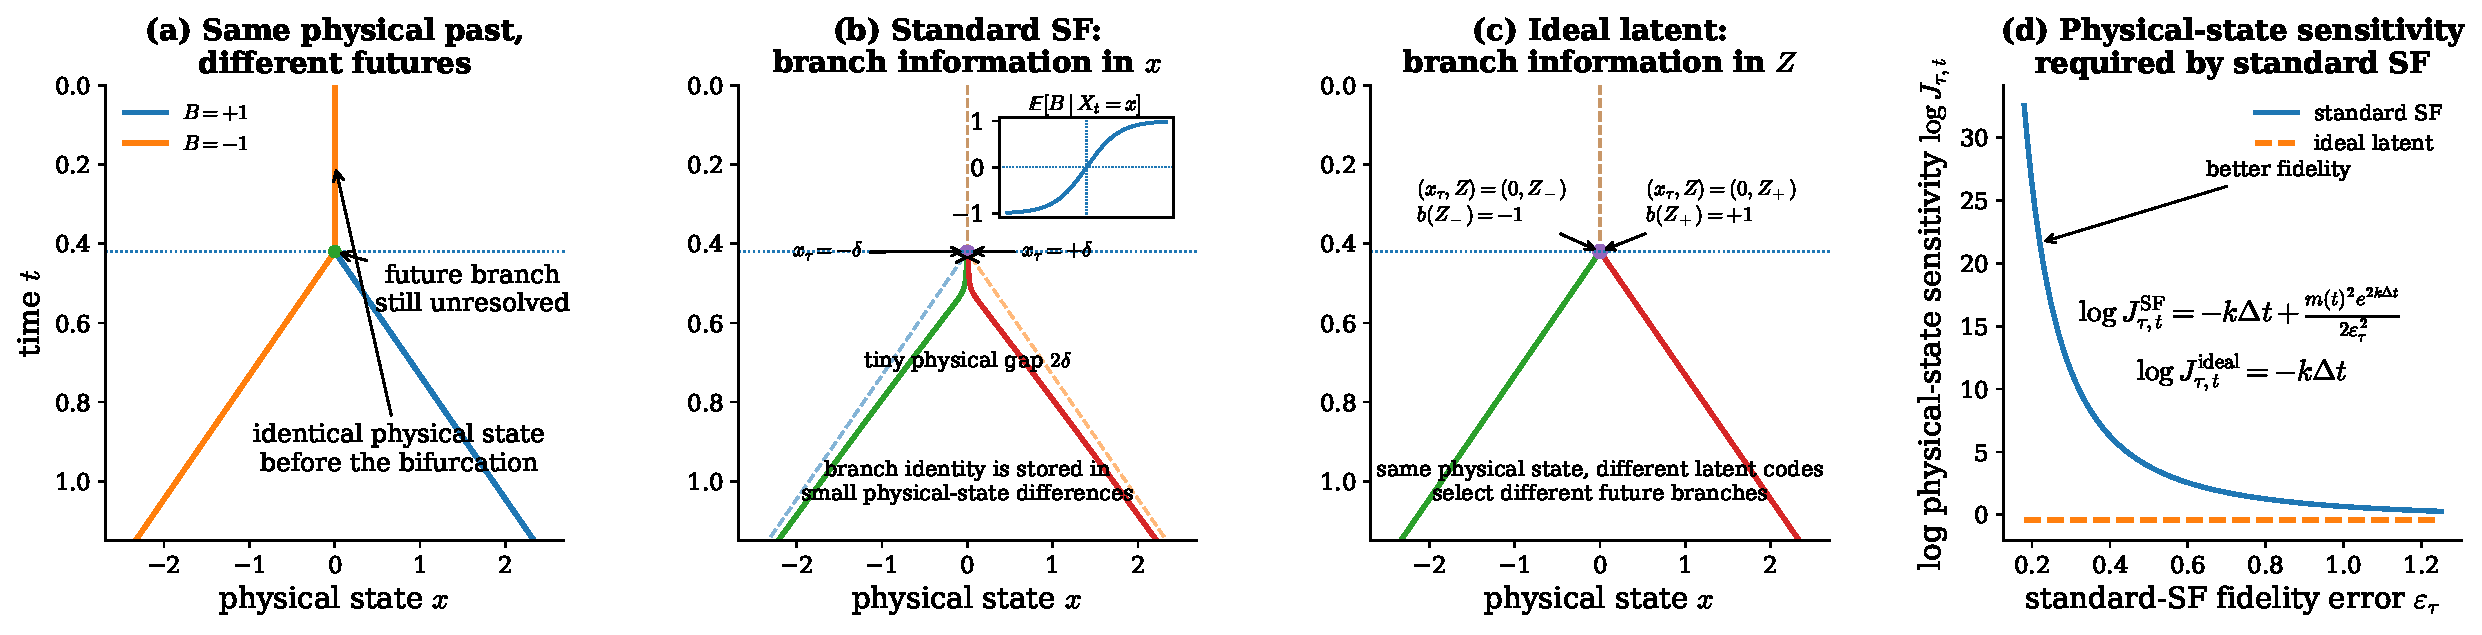
\includegraphics[width=1.005\linewidth]{figures/bif_example.pdf}
            \caption{(a) Two futures share the same physical state up to the bifurcation time $\tau$.
(b) In non-latent SF, branch identity must be encoded by small differences in the physical state $x$, making the branch signal increasingly sharp as the Gaussian tube narrows.
(c) An ideal latent realization instead carries branch identity in $Z$, allowing the same physical state $X_\tau=0$ to generate either future.
(d) Accordingly, the standard-SF physical-state sensitivity grows as
$J_{\tau,t}^{\mathrm{SF}}\sim \exp(C/\varepsilon_\tau^2)$
as the  fidelity error $\varepsilon_\tau\to0$, while the ideal latent realization retains
$J_{\tau,t}^{\mathrm{ideal}}=e^{-k(t-\tau)}$. }
    \label{fig:motivate}
\end{figure}

{\bf A bifurcation example.} Fix an observed history $H=h$. Let $B\in\{-1,+1\}$ be equally likely
conditional on $h$, and consider the two future trajectories
\begin{equation}
    \xi_B(t)=B\,m(t),
    \qquad t\in[0,T],
    \label{eq:bifurcation_paths}
\end{equation}
where $m:[0,T]\to[0,\infty)$ is absolutely continuous on $[0,T]$,
continuously differentiable on $(\tau,T]$, satisfies
$m(t)=0$ for $t\leq\tau$, and $m(t)>0$ for $t>\tau$.
Thus the two futures share the same physical trajectory up to the
bifurcation time $\tau$ and separate afterward.

Let
$k>0$ and $\sigma_0>0$, and consider the branch-conditioned fields
\begin{equation}
    g_B(x,t)
    =
    \dot\xi_B(t)-k\bigl(x-\xi_B(t)\bigr).
    \label{eq:bifurcation_sf_conditional_field}
\end{equation}
Define
$\sigma_t^2=\sigma_0^2e^{-2kt},$
$q(t)=\dot m(t)+km(t)$.

\begin{vsfproposition}[Fidelity-sensitivity tradeoff]
\label{prop_motivate} Assume that the population optimum of the SF objective is attained.  Then, we have the following results.

(i) The optimal SF marginal field is
\begin{equation}
    v_{\mathrm{SF}}^\star(x,t)
    =
    -kx
    +
    q(t)
    \tanh\!\left(
        \frac{x\,m(t)}{\sigma_t^2}
    \right).
    \label{eq:bifurcation_sf_field}
\end{equation}
At the bifurcation time,
$P_{\tau}^{\mathrm{SF}}
    =
    \mathcal N(0,\sigma_\tau^2),$
    $P_{\tau}^{\mathrm{data}}
    =
    \delta_0,$
and therefore
\begin{equation}
    \varepsilon_\tau
    :=
    W_2\!\left(
        P_{\tau}^{\mathrm{SF}},
        P_{\tau}^{\mathrm{data}}
    \right)
    =
    \sigma_\tau.
    \label{eq:bifurcation_sf_fidelity}
\end{equation}

(ii) $x(t)\equiv0$ is a trajectory of
$v_{\mathrm{SF}}^\star$. 
  If
$\Phi_{\tau,t}^{\mathrm{SF}}$ denotes its flow map, then for every
$t>\tau$,
\begin{equation}
    J_{\tau,t}^{\mathrm{SF}}
    :=
    \left.
    \frac{\partial
        \Phi_{\tau,t}^{\mathrm{SF}}(x)}
        {\partial x}
    \right|_{x=0}
    =
    \exp\!\left[
        -k(t-\tau)
        +
        \frac{
            m(t)^2e^{2k(t-\tau)}
        }{
            2\varepsilon_\tau^2
        }
    \right].
    \label{eq:bifurcation_fidelity_sensitivity}
\end{equation}
Hence, for every fixed $t>\tau$ with $m(t)>0$, and with
$k$, $m$, and $\tau$ fixed,
\begin{equation}
    \sigma_0\downarrow0
    \quad\Longleftrightarrow\quad
    \varepsilon_\tau\downarrow0
    \quad\Longrightarrow\quad
    J_{\tau,t}^{\mathrm{SF}}\to\infty.
    \label{eq:bifurcation_tradeoff_limit}
\end{equation}
\end{vsfproposition} 
Thus, in this example, standard SF faces
an explicit fidelity-sensitivity tradeoff: making the physical tube
arbitrarily close to the common target state forces the population
marginal field near the branch separator to become arbitrarily sensitive
to physical-state perturbations.

\paragraph{Proof.}
For branch $B$, plugging $\xi_B(t)=Bm(t)$ into
\eqref{eq:bifurcation_sf_conditional_field} gives
\begin{equation}
    g_B(x,t)
    =
    -kx+Bq(t),
    \qquad
    q(t)=\dot m(t)+km(t).
    \label{eq:bifurcation_sf_branch_field}
\end{equation}

We first derive the branch-conditioned  marginal field. Let
$E_t=X_t-\xi_B(t)$. From
\eqref{eq:bifurcation_sf_conditional_field},
\begin{equation}
    \dot E_t
    =
    \dot X_t-\dot\xi_B(t)
    =
    -kE_t.
\end{equation}
Hence
\begin{equation}
    E_t=e^{-kt}E_0.
\end{equation}
Since $\xi_B(0)=0$ and the standard SF construction uses
$X_0\sim\mathcal N(0,\sigma_0^2)$, we have
$E_0\sim\mathcal N(0,\sigma_0^2)$. Consequently,
\begin{equation}
    X_t\mid B
    \sim
    \mathcal N\!\left(
        Bm(t),
        \sigma_t^2
    \right),
    \qquad
    \sigma_t^2=\sigma_0^2e^{-2kt}.
    \label{eq:bifurcation_sf_branch_marginal}
\end{equation}

Under conditional flow matching, the population-optimal
marginal field is the conditional expectation of the branch-conditioned
target:
\begin{equation}
    v_{\mathrm{SF}}^\star(x,t)
    =
    \mathbb E[
        g_B(X_t,t)\mid X_t=x],
    \label{eq:bifurcation_sf_conditional_mean}
\end{equation}
where the corresponding marginal probability path is:
\begin{equation}
    P_t^{\mathrm{SF}}
    =
    \frac12\mathcal N(m(t),\sigma_t^2)
    +
    \frac12\mathcal N(-m(t),\sigma_t^2).
    \label{eq:bifurcation_sf_mixture}
\end{equation}

Using \eqref{eq:bifurcation_sf_branch_field},
\begin{equation}
    v_{\mathrm{SF}}^\star(x,t)
    =
    -kx
    +
    q(t)\,
    \mathbb E[B\mid X_t=x].
    \label{eq:bifurcation_sf_branch_mean}
\end{equation}
It remains to evaluate the posterior mean of $B$. From
\eqref{eq:bifurcation_sf_branch_marginal} and the equal branch
probabilities,
\begin{equation}
    \frac{
        \mathbb P(B=+1\mid X_t=x)
    }{
        \mathbb P(B=-1\mid X_t=x)
    }
    =
    \frac{
        \exp\!\left(
            -(x-m(t))^2/(2\sigma_t^2)
        \right)
    }{
        \exp\!\left(
            -(x+m(t))^2/(2\sigma_t^2)
        \right)
    }.
\end{equation}
Therefore
\begin{align}
    \log
    \frac{
        \mathbb P(B=+1\mid X_t=x)
    }{
        \mathbb P(B=-1\mid X_t=x)
    }
    &=
    \frac{
        (x+m(t))^2-(x-m(t))^2
    }{
        2\sigma_t^2
    }
    \notag\\
    &=
    \frac{2x\,m(t)}{\sigma_t^2}.
\end{align}
For a random variable taking values in $\{-1,+1\}$, this gives:
\begin{equation}
    \mathbb E[B\mid X_t=x]
    =
    \tanh\!\left(
        \frac{x\,m(t)}{\sigma_t^2}
    \right).
\end{equation}
Substitution into
\eqref{eq:bifurcation_sf_branch_mean} allows us to obtain
\eqref{eq:bifurcation_sf_field}.

At the bifurcation time, $m(\tau)=0$. Hence
\eqref{eq:bifurcation_sf_branch_marginal} gives
\begin{equation}
    P_{\tau}^{\mathrm{SF}}
    =
    \mathcal N(0,\sigma_\tau^2),
\end{equation}
whereas the two noiseless target branches both satisfy
$\xi_B(\tau)=0$, so
\begin{equation}
    P_{\tau}^{\mathrm{data}}=\delta_0.
\end{equation}
The only coupling between a distribution and a Dirac mass sends every
sample to the location of the Dirac mass. Therefore
\begin{align}
    W_2^2\!\left(
        P_{\tau}^{\mathrm{SF}},
        \delta_0
    \right)
    &=
    \mathbb E|X_\tau|^2
    = \sigma_\tau^2.
\end{align}
Thus
$W_2\!\left(
        P_{\tau}^{\mathrm{SF}},
        P_{\tau}^{\mathrm{data}}
    \right)  =
    \sigma_\tau,$
which is precisely
\eqref{eq:bifurcation_sf_fidelity}.

We next compute the sensitivity of the population SF near
the branch separator. By symmetry,
$v_{\mathrm{SF}}^\star(0,t)=0,$
so $x(t)\equiv0$ is a trajectory. Differentiating
\eqref{eq:bifurcation_sf_field} with respect to $x$ gives
\begin{equation}
    \partial_xv_{\mathrm{SF}}^\star(x,t)
    =
    -k
    +
    \frac{
        m(t)q(t)
    }{
        \sigma_t^2
    }
    \operatorname{sech}^2\!\left(
        \frac{x\,m(t)}{\sigma_t^2}
    \right).
\end{equation}
Along the central trajectory,
\begin{equation}
    \partial_xv_{\mathrm{SF}}^\star(0,t)
    =
    -k
    +
    \frac{
        m(t)[\dot m(t)+km(t)]
    }{
        \sigma_t^2
    }.
    \label{eq:bifurcation_sf_central_jacobian}
\end{equation}

Let
\begin{equation}
    J_{\tau,t}^{\mathrm{SF}}
    =
    \left.
    \frac{\partial
        \Phi_{\tau,t}^{\mathrm{SF}}(x)}
        {\partial x}
    \right|_{x=0}.
\end{equation}
The variational equation for the one-dimensional ODE flow gives
\begin{equation}
    \frac{d}{dt}J_{\tau,t}^{\mathrm{SF}}
    =
    \partial_xv_{\mathrm{SF}}^\star(0,t)
    J_{\tau,t}^{\mathrm{SF}},
    \qquad
    J_{\tau,\tau}^{\mathrm{SF}}=1.
\end{equation}
Therefore
\begin{equation}
    J_{\tau,t}^{\mathrm{SF}}
    =
    \exp\!\left(
        \int_\tau^t
        \partial_xv_{\mathrm{SF}}^\star(0,s)\,ds
    \right).
    \label{eq:bifurcation_sf_variational_solution}
\end{equation}

Since $\sigma_s^2=\sigma_0^2e^{-2ks}$,
\begin{equation}
    \frac{d}{ds}
    \left(
        \frac{m(s)^2}{2\sigma_s^2}
    \right)
    =
    \frac{
        m(s)[\dot m(s)+km(s)]
    }{
        \sigma_s^2
    }.
\end{equation}
Using $m(\tau)=0$ in
\eqref{eq:bifurcation_sf_central_jacobian}, we obtain
\begin{align}
    \int_\tau^t
    \partial_xv_{\mathrm{SF}}^\star(0,s)\,ds
    &=
    -k(t-\tau)
    +
    \int_\tau^t
    \frac{
        m(s)[\dot m(s)+km(s)]
    }{
        \sigma_s^2
    }
    ds
    \notag\\
    &=
    -k(t-\tau)
    +
    \frac{m(t)^2}{2\sigma_t^2}.
\end{align}

From
$\sigma_t^2=\sigma_\tau^2e^{-2k(t-\tau)}$ and
$\varepsilon_\tau=\sigma_\tau$, we further obtain
\begin{equation}
    \frac{m(t)^2}{2\sigma_t^2}
    =
    \frac{
        m(t)^2e^{2k(t-\tau)}
    }{
        2\varepsilon_\tau^2
    }.
\end{equation}
Using these and
\eqref{eq:bifurcation_sf_variational_solution}, we  obtain
\eqref{eq:bifurcation_fidelity_sensitivity}. 

Finally, for every fixed
$t>\tau$ with $m(t)>0$, the second term in the exponent diverges as
$\varepsilon_\tau\to0$, which proves
\eqref{eq:bifurcation_tradeoff_limit}.

\begin{vsfcorollary}
\label{cor:sf_fidelity_robustness_lower_bound}
Under the assumptions of
Proposition~\ref{prop_motivate}, suppose that for
some fixed $t>\tau$ the SF sensitivity is required to
satisfy
$J_{\tau,t}^{\mathrm{SF}}\leq J_{\max}$ for some threshold $J_{\max}$. Then,
whenever this constraint is feasible, it is necessary that
$J_{\max}>e^{-k(t-\tau)}$, and
\begin{equation}
    \varepsilon_\tau
    \geq
    \frac{
        m(t)e^{k(t-\tau)}
    }{
        \sqrt{
            2\left[
                \log J_{\max}+k(t-\tau)
            \right]
        }
    }.
    \label{eq:sf_fidelity_lower_bound}
\end{equation}
\end{vsfcorollary}
Thus, within this model,  keeping the
physical-state sensitivity bounded by a threshold imposes a strictly positive lower bound on
the fidelity error.


\begin{tcolorbox}[
  colback=parchment,
  colframe=sandborder,
  boxrule=0.1pt,
  left=8pt,
  right=8pt,
  top=0.3pt,
  bottom=0.3pt
]
\centering
Proposition \ref{prop_motivate} reveals a limitation in  SF:  the physical state must simultaneously track the shared trajectory and encode  future branch information, so near a bifurcation improved physical fidelity necessarily causes branch selection to be more sensitive to state perturbations.
\end{tcolorbox}

%Along the common stem, both true future branches satisfy $X_t=0$, whereas the SF state retains variance $\sigma_t^2$. Shrinking this physical tube improves fidelity, but the marginal field must then infer opposite branch directions from increasingly nearby physical states. 
%The factor $\tanh\!\left(\frac{x\,m(t)}\sigma_t^2}\right)$ makes this explicit: as $\sigma_t$ decreases, the branch-separating transition around $x=0$ becomes increasingly sharp. 
\Eqref{eq:bifurcation_fidelity_sensitivity} quantifies the resulting
fidelity--sensitivity tradeoff.

\paragraph{Why introducing a latent model?} While latent variable models are more expressive and can improve performance in general,
the preceding example gives a clear motivation to separate the stochastic branch
information from the physical state, motivating the use of latent SF models.
In the following, we show that there exists such a latent model, without making
a claim about the learned model itself. 
Let $Z\sim\mathcal N(0,1)$ be sampled once for the
trajectory, define
\begin{equation}
b(Z)
=
\begin{cases}
+1, & Z\geq0,\\
-1, & Z<0,
\end{cases}
\label{eq:bifurcation_ideal_branch_code}
\end{equation}
and use the latent-conditioned physical-time field
\begin{equation}
v_{\mathrm{ideal}}(x,t,Z)
=
-kx+b(Z)q(t)
=
b(Z)\dot m(t)
-
k\bigl(x-b(Z)m(t)\bigr),
\label{eq:bifurcation_ideal_field}
\end{equation}
where $q(t)=\dot m(t)+km(t)$ as above.
Thus, conditional on the latent branch code $b(Z)$,
$v_{\mathrm{ideal}}$ has exactly the same form as the branch-conditioned
SF field in \eqref{eq:bifurcation_sf_branch_field}; the difference is that
the branch information is now supplied by the latent variable rather than
having to be inferred from the physical state.

Starting from the  observed state $X_0=0$, this field gives
\begin{equation}
X_t=b(Z)m(t),
\label{eq:bifurcation_ideal_path}
\end{equation}
and hence realizes the target conditional path law
\begin{equation}
\operatorname{Law}(X_\cdot\mid H=h)
=
\frac12\delta_{\xi_+}
+
\frac12\delta_{\xi_-}.
\label{eq:bifurcation_ideal_path_law}
\end{equation}
In particular,
$W_2\left(
P_{\tau}^{\mathrm{ideal}},
P_{\tau}^{\mathrm{data}}
\right)
=0.$
Furthermore,
\begin{equation}
\partial_xv_{\mathrm{ideal}}(x,t,Z)=-k,
\end{equation}
so, for fixed $Z$,
\begin{equation}
\frac{\partial
\Phi_{\tau,t}^{\mathrm{ideal}}(x,Z)}
{\partial x}
=
e^{-k(t-\tau)}.
\label{eq:bifurcation_ideal_sensitivity}
\end{equation}

Indeed, define
$E_t=X_t-b(Z)m(t).$
Using \eqref{eq:bifurcation_ideal_field},
\begin{align}
\dot E_t
&=
\dot X_t-b(Z)\dot m(t)
=
-k\bigl(X_t-b(Z)m(t)\bigr)
=
-kE_t.
\end{align}
Since $X_0=0$ and $m(0)=0$, we have $E_0=0$, and therefore
$E_t=0$ for every $t$, which proves
\eqref{eq:bifurcation_ideal_path}. Since
$\mathbb P(b(Z)=+1)=\mathbb P(b(Z)=-1)=1/2$, this proves
\eqref{eq:bifurcation_ideal_path_law}; since $m(\tau)=0$, we have $W_2\left(
P_{\tau}^{\mathrm{ideal}},
P_{\tau}^{\mathrm{data}}
\right)
=0$.

More generally, for fixed $Z$, solving
\eqref{eq:bifurcation_ideal_field} from time $\tau$ with
$X_\tau=x$ gives
\begin{equation}
\Phi_{\tau,t}^{\mathrm{ideal}}(x,Z)
=
e^{-k(t-\tau)}x+b(Z)m(t),
\end{equation}
where we used $m(\tau)=0$. Differentiating with respect to $x$
gives \eqref{eq:bifurcation_ideal_sensitivity}.
This construction shows what becomes possible once branch information
need not be stored in the physical coordinate: the physical state can remain
on the common stem, while the latent variable distinguishes the future
trajectories.

\paragraph{Connection to rollout robustness.}
The sensitivity calculation also gives a direct local mechanism to understand rollout
error amplification. If a small physical-state perturbation $\delta$ is
introduced at the bifurcation, then standard SF satisfies
\begin{equation}
\Phi_{\tau,t}^{\mathrm{SF}}(\delta)
-
\Phi_{\tau,t}^{\mathrm{SF}}(0)
=
J_{\tau,t}^{\mathrm{SF}}\delta
+
o(\delta),
\label{eq:bifurcation_sf_perturbation}
\end{equation}
whereas the ideal latent construction satisfies, for fixed $Z$,
\begin{equation}
\Phi_{\tau,t}^{\mathrm{ideal}}(x+\delta,Z)
-
\Phi_{\tau,t}^{\mathrm{ideal}}(x,Z)
=
e^{-k(t-\tau)}\delta.
\label{eq:bifurcation_ideal_perturbation}
\end{equation}
Thus, in this example the same mechanism behind the 
fidelity-sensitivity tradeoff also provides a mechanism by which standard
non-latent SF can amplify physical-state rollout errors near a branch
separator. By contrast, once the branch information is encoded by the
latent variable in the idealized construction, physical-state perturbations
are governed only by the original stabilizing dynamics and are contracted
at rate $e^{-k(t-\tau)}$.

\paragraph{This motivates VSF.}
The proposition and discussions above identify a bottleneck of
standard non-latent SF, and the idealized latent construction shows
how that bottleneck can in principle be removed by carrying future-specific
information outside the physical state.
This observation motivates VSF. Rather than requiring the physical state alone
to carry all residual uncertainty needed for later bifurcation, VSF conditions
the physical-time velocity field on an additional latent variable sampled once
per forecast. 
\begin{tcolorbox}[
  colback=parchment,
  colframe=sandborder,
  boxrule=0.1pt,
  left=8pt,
  right=8pt,
  top=0.3pt,
  bottom=0.3pt
]
\centering
The variational  framework of VSF provides a principled way to associate
observed future dynamics with {\it learned latent codes} during training, while the learned prior
provides the corresponding randomness at inference. 
\end{tcolorbox}
The goal is therefore to
learn a distribution of coherent physical-time dynamics in which distinct
future continuations can be represented without requiring increasingly
sensitive separation in the physical state itself.




\clearpage
\section{A variational objective for clean streaming trajectories}
\label{sec:clean_velocity_elbo}


\begin{vsfproposition}[Conditional-velocity evidence lower bound]
\label{prop:velocity_elbo}
Fix a training tuple $(\vu_s,\vx_s,s,\vh)$ constructed from the physical-time
path in Eqs.~\ref{eq:physical_time_interpolation}--
\ref{eq:physical_time_velocity}.  Let $p(\vz)$ be the latent prior, 
$p_{\vtheta}(\vu_s\mid\vx_s,s,\vh,\vz)$ be a conditional velocity
likelihood, and $q_{\vphi}(\vz\mid\vu_s,\vx_s,s,\vh)$ be a
variational posterior.  Define the conditional velocity evidence by
\begin{equation}
  p_{\vtheta}(\vu_s\mid\vx_s,s,\vh)
  :=
  \int
  p_{\vtheta}(\vu_s\mid\vx_s,s,\vh,\vz)
  p(\vz)\,d\vz.
  \label{eq:conditional_velocity_evidence}
\end{equation}
Assume that the displayed quantities are finite, that the evidence is
positive, and that the variational posterior is absolutely continuous with
respect to the exact model posterior.
Then
\begin{align}
  \log p_{\vtheta}(\vu_s\mid\vx_s,s,\vh)
  &\geq
  \mathcal E_{\vtheta,\vphi}(\vu_s,\vx_s,s,\vh)
  \notag\\
  &:={}
  \E_{q_{\vphi}}
  \!\left[
    \log p_{\vtheta}(\vu_s\mid\vx_s,s,\vh,\vz)
  \right]
  \notag
  -
  \KL\!\left(
    q_{\vphi}(\vz\mid\vu_s,\vx_s,s,\vh)
    \,\Vert\,
    p(\vz)
  \right).
  \label{eq:pointwise_velocity_elbo}
\end{align}
\end{vsfproposition}

\paragraph{Proof.}
Inserting the variational posterior into the conditional evidence gives
\begin{align*}
  \log p_{\vtheta}(\vu_s\mid\vx_s,s,\vh)
  &={}
  \log\int
  q_{\vphi}(\vz\mid\vu_s,\vx_s,s,\vh)
  \frac{
    p_{\vtheta}(\vu_s\mid\vx_s,s,\vh,\vz)p(\vz)
  }{
    q_{\vphi}(\vz\mid\vu_s,\vx_s,s,\vh)
  }\,d\vz
  \\
  &={}
  \log\E_{q_{\vphi}(\vz\mid\vu_s,\vx_s,s,\vh)}\!\left[
    \frac{
      p_{\vtheta}(\vu_s\mid\vx_s,s,\vh,\vz)p(\vz)
    }{
      q_{\vphi}(\vz\mid\vu_s,\vx_s,s,\vh)
    }
  \right]
  \\
  &\geq
  \E_{q_{\vphi}(\vz\mid\vu_s,\vx_s,s,\vh)}\!\left[
    \log p_{\vtheta}(\vu_s\mid\vx_s,s,\vh,\vz)
    +\log p(\vz)
    -\log q_{\vphi}(\vz\mid\vu_s,\vx_s,s,\vh)
  \right]
  \\
  &={}
  \E_{q_{\vphi}(\vz\mid\vu_s,\vx_s,s,\vh)}\!\left[
    \log p_{\vtheta}(\vu_s\mid\vx_s,s,\vh,\vz)
  \right]
  \\
  &\quad
  -\KL\!\left(
    q_{\vphi}(\vz\mid\vu_s,\vx_s,s,\vh)
    \,\Vert\,
    p(\vz)
  \right)
  \\
  &={}
  \mathcal E_{\vtheta,\vphi}(\vu_s,\vx_s,s,\vh),
\end{align*}
where Jensen's inequality gives the lower bound. 
%and the final equality is Eq.~\ref{eq:pointwise_velocity_elbo}.

For completeness, Bayes' rule gives the exact conditional posterior
\begin{equation*}
  p_{\vtheta}(\vz\mid\vu_s,\vx_s,s,\vh)
  =
  \frac{
    p_{\vtheta}(\vu_s\mid\vx_s,s,\vh,\vz)p(\vz)
  }{
    p_{\vtheta}(\vu_s\mid\vx_s,s,\vh)
  }.
\end{equation*}
Therefore,
\begin{align*}
  &\KL\!\left(
    q_{\vphi}(\vz\mid\vu_s,\vx_s,s,\vh)
    \,\Vert\,
    p_{\vtheta}(\vz\mid\vu_s,\vx_s,s,\vh)
  \right)
  \\
  &={}
  \E_{q_{\vphi}(\vz\mid\vu_s,\vx_s,s,\vh)}\!\left[
    \log\frac{
      q_{\vphi}(\vz\mid\vu_s,\vx_s,s,\vh)
    }{
      p_{\vtheta}(\vu_s\mid\vx_s,s,\vh,\vz)p(\vz)
    }
  \right]
  +\log p_{\vtheta}(\vu_s\mid\vx_s,s,\vh)
  \\
  &={}
  \log p_{\vtheta}(\vu_s\mid\vx_s,s,\vh)
  -\mathcal E_{\vtheta,\vphi}(\vu_s,\vx_s,s,\vh),
\end{align*}
which proves the variational gap where $p_{\vtheta}(\vz\mid\vu_s,\vx_s,s,\vh)$ is the exact model
posterior.  Equality holds if and only if the variational and exact posteriors
agree almost everywhere. \hfill$\square$

\paragraph{Equivalent local conditioning.}
For a realized training tuple, $\vu_s$ is the prediction target of the
conditional velocity likelihood
$p_{\vtheta}(\vu_s\mid\vx_s,s,\vh,\vz)$, rather than one of its
conditioning variables. It is provided only to the training-time variational
posterior $q_{\vphi}$. For the piecewise-linear physical-time path and
$s\in I_k := [s_k, s_{k+1})$,
\begin{equation}
  \vu_s
  =
  P\bigl(\vx_{m+k+1}-\vx_{m+k}\bigr).
  \label{eq:local_velocity_endpoints}
\end{equation}
Conversely, because $s$ determines both $k$ and $\alpha_s$, the two endpoints
can be recovered from $(\vu_s,\vx_s,s)$ according to
\begin{equation}
  \vx_{m+k}
  =
  \vx_s-\frac{\alpha_s}{P}\vu_s,
  \qquad
  \vx_{m+k+1}
  =
  \vx_s+\frac{1-\alpha_s}{P}\vu_s.
  \label{eq:recover_local_endpoints}
\end{equation}
Therefore, on the support of the piecewise-linear interpolation and for almost
every $s$,
\begin{equation}
  (\vu_s,\vx_s,s)
  \quad\Longleftrightarrow\quad
  (\vx_{m+k},\vx_{m+k+1},\vx_s,s).
  \label{eq:local_evidence_equivalence}
\end{equation}
The local endpoint representation thus provides the same conditioning
information to the variational posterior as $(\vu_s,\vx_s,s)$. This
reparameterization does not alter the conditioning variables
$(\vx_s,s,\vh)$ of the velocity likelihood. Accordingly, the local
variational posterior can equivalently be parameterized as
\begin{equation}
  q_{\vphi}^{\mathrm{loc}}\!\left(
    \vz
    \mid
    \vx_{m+k},
    \vx_{m+k+1},
    \vx_s,
    s,
    \vh
  \right).
  \label{eq:local_variational_encoder}
\end{equation}


\clearpage

\section{Population Energy Reconstruction and Energy-Distance Control}
\label{sec:population_energy_control}

Fix $(\vx_s,s,\vh)$ and draw
\begin{align*}
  \vu,\vu'
  &\stackrel{\mathrm{iid}}{\sim}
  p_{\mathrm{data}}(\cdot\mid\vx_s,s,\vh),
  \quad
  \vz,\vz'\mid\vu
  \stackrel{\mathrm{iid}}{\sim}
  q_{\vphi}(\cdot\mid\vu,\vx_s,s,\vh),
  \quad
  \widetilde{\vz},\widetilde{\vz}'
  \stackrel{\mathrm{iid}}{\sim}p(\vz),
\end{align*}
where all draws are independent except for the displayed conditioning. Define
\begin{align*}
  \widehat{\vu}
  &:=
  \vv_{\vtheta}(\vx_s,s,\vh,\vz),
  &
  \widehat{\vu}'
  &:=
  \vv_{\vtheta}(\vx_s,s,\vh,\vz'),
  \\
  \widetilde{\vu}
  &:=
  \vv_{\vtheta}(\vx_s,s,\vh,\widetilde{\vz}),
  &
  \widetilde{\vu}'
  &:=
  \vv_{\vtheta}(\vx_s,s,\vh,\widetilde{\vz}').
\end{align*}
For a realized target $\vu$, let
\begin{equation}
  S_\alpha(\vu)
  :=
  \E\!\left[
    \left\|\widehat{\vu}-\vu\right\|_2^\alpha
    \,\middle|\,\vu
  \right]
  -
  \frac12
  \E\!\left[
    \left\|\widehat{\vu}-\widehat{\vu}'\right\|_2^\alpha
    \,\middle|\,\vu
  \right].
  \label{eq:vsf_population_energy_reconstruction}
\end{equation}
This is the population counterpart of the generalized energy reconstruction
in Eq.~\ref{eq:vsf_energy_score}; replacing its expectations with the $M$
posterior samples gives the finite-ensemble V-statistic
$\mathcal L_{\mathrm{ES}}$.

The energy distance between the prior-predictive velocity and the true
conditional velocity is
\begin{equation}
  D_\alpha(\widetilde{\vu},\vu)
  :=
  2\E\left\|\widetilde{\vu}-\vu\right\|_2^\alpha
  -
  \E\left\|\widetilde{\vu}-\widetilde{\vu}'\right\|_2^\alpha
  -
  \E\left\|\vu-\vu'\right\|_2^\alpha.
  \label{eq:vsf_prior_energy_distance}
\end{equation}

Define the aggregate posterior
\begin{equation}
    \overline q_{\vphi}(\vz\mid\vx_s,s,\vh)
    :=
    \E_{\vu\sim
    p_{\mathrm{data}}(\cdot\mid\vx_s,s,\vh)}
    \left[
        q_{\vphi}(\vz\mid\vu,\vx_s,s,\vh)
    \right].
    \label{eq:aggregate_posterior}
\end{equation}

\begin{vsfproposition}[Prior-predictive energy-distance control]
\label{prop:vsf_aggregate_energy_bound}
If $0<\alpha<2$, all expectations above are finite, and
\(
  \overline q_{\vphi}(\vz\mid\vx_s,s,\vh)=p(\vz)
  \quad\text{for almost every }\vz,
\)
then
\begin{equation}
  \frac12D_\alpha(\widetilde{\vu},\vu)
  \leq
  \E_{\vu\sim p_{\mathrm{data}}(\cdot\mid\vx_s,s,\vh)}
  \!\left[S_\alpha(\vu)\right]
  \label{eq:vsf_aggregate_energy_bound}
\end{equation}
\end{vsfproposition}

\paragraph{Proof.}
For $\rho_\alpha(a,b)=\|a-b\|_2^\alpha$ and $0<\alpha<2$, there exist a
Hilbert space $\mathcal H_\alpha$ and a feature map $\psi_\alpha$ such that
\begin{equation*}
  \rho_\alpha(a,b)
  =
  \left\|\psi_\alpha(a)-\psi_\alpha(b)\right\|_{\mathcal H_\alpha}^2
\end{equation*}
\citep{gneiting2007strictly,szekely2013energy}. Define
\begin{equation*}
  m_q(\vu)
  :=
  \E[\psi_\alpha(\widehat{\vu})\mid\vu],
  \qquad
  m_p
  :=
  \E[\psi_\alpha(\widetilde{\vu})].
\end{equation*}
Aggregate posterior--prior alignment and
\(\overline q_{\vphi}(\vz\mid\vx_s,s,\vh)
    :=
    \E_{\vu\sim p_{\mathrm{data}}(\cdot\mid\vx_s,s,\vh)}
    \!\left[
        q_{\vphi}(\vz\mid\vu,\vx_s,s,\vh)
    \right]\) imply

\begin{equation*}
  m_p
  =
  \E_{\vu\sim p_{\mathrm{data}}(\cdot\mid\vx_s,s,\vh)}
  [m_q(\vu)].
\end{equation*}
The energy-score identities and Jensen's inequality now give
\begin{align*}
  \frac12D_\alpha(\widetilde{\vu},\vu)
  &=
  \left\|
    \E_{\vu}
    \!\left[m_q(\vu)-\psi_\alpha(\vu)\right]
  \right\|_{\mathcal H_\alpha}^2
  \\
  &\leq
  \E_{\vu}
  \!\left[
    \left\|m_q(\vu)-\psi_\alpha(\vu)\right\|_{\mathcal H_\alpha}^2
  \right]
  =
  \E_{\vu}[S_\alpha(\vu)],
\end{align*}
where $\vu\sim p_{\mathrm{data}}(\cdot\mid\vx_s,s,\vh)$ in each
expectation. \hfill$\square$


The expected energy reconstruction upper-bounds half the energy distance between the decoded aggregate posterior and the true conditional velocity law. Thus, reducing the reconstruction objective controls a distribution-level discrepancy, rather than only an error in the conditional mean.



\paragraph{Interpretation of aggregate alignment.}
For each fixed context $c=(\vx_s,s,\vh)$, the equality says that averaging
the encodings of true velocities at that context gives the prior. It can hold
in several circumstances:
\begin{itemize}[leftmargin=*,nosep]
  \item \textbf{Ideal inference and model fit.}
  If $q_{\vphi}(\vz\mid\vu,c)$ is the exact model posterior and
  $p_{\vtheta}(\vu\mid c)=p_{\mathrm{data}}(\vu\mid c)$, then Bayes' rule
  gives
  \begin{equation*}
    \overline q_{\vphi}(\vz\mid c)
    =
    \int
    p_{\vtheta}(\vz\mid\vu,c)
    p_{\vtheta}(\vu\mid c)\,d\vu
    =
    p(\vz).
  \end{equation*}
  This is the intended justification for the assumption
  \citep{hoffman2016elbo}.

  \item \textbf{Aggregate-matching training.}
  A penalty on the aggregate posterior can encourage approximate equality,
  although finite-capacity training does not guarantee exact equality
  \citep{tolstikhin2017wasserstein}.

  \item \textbf{Posterior collapse.}
  The encoder can output $q_{\vphi}(\vz\mid\vu,c)=p(\vz)$ for every $\vu$,
  which also satisfies the equality.
\end{itemize}



% \subsection{Proper-scoring analysis of the generalized energy loss}
% \label{sec:crps_mae_propriety}

% Fix the local conditioning variables $(\vx_s,s,\vh)$.  Let
% $\mathsf G_s(\cdot\mid\vx_s,s,\vh)$ denote the true conditional law of
% $\vu_s$, and let $\mathsf F_s(\cdot\mid\vx_s,s,\vh)$ be a forecast law that
% does not depend on the realized target $\vu_s$.  In particular, the
% prior-predictive VSF law has the form
% \[
%   \mathsf F_{\vtheta,s}(\cdot\mid\vx_s,s,\vh)
%   :=\operatorname{Law}_{\vz\sim p(\vz)}\!\left[
%     \vv_{\vtheta}(\vx_s,s,\vh,\vz)
%   \right].
% \]
% For independent draws
% $\widehat{\vu}_s^{(1)},\ldots,\widehat{\vu}_s^{(M)}\sim\mathsf F_s$, the
% $\alpha=1$ empirical loss is
% \begin{equation}
%   \widehat{\mathcal L}_{1,M}^{(\lambda)}
%   =\frac{1}{M}\sum_{i=1}^{M}
%     \left\|\widehat{\vu}_s^{(i)}-\vu_s\right\|_2
%   -\frac{\lambda}{M^2}\sum_{i,j=1}^{M}
%     \left\|\widehat{\vu}_s^{(i)}-
%       \widehat{\vu}_s^{(j)}\right\|_2.
%   \label{eq:crps_mae_training_loss}
% \end{equation}
% More generally, for $\alpha>0$, define
% \begin{equation}
%   \widehat{\mathcal L}_{\alpha,M}^{(\lambda)}
%   :=\frac1M\sum_{i=1}^M
%        \left\|\widehat{\vu}_s^{(i)}-\vu_s\right\|_2^\alpha
%     -\frac{\lambda}{M^2}\sum_{i,j=1}^M
%        \left\|\widehat{\vu}_s^{(i)}-
%          \widehat{\vu}_s^{(j)}\right\|_2^\alpha.
%   \label{eq:generalized_crps_training_loss}
% \end{equation}
% Equation~\ref{eq:crps_mae_training_loss} is the case $\alpha=1$.
% Let
% $\widehat{\mathsf F}_{s,M}:=M^{-1}\sum_{i=1}^M
% \delta_{\widehat{\vu}_s^{(i)}}$ denote the empirical forecast law. At $\lambda=1/2$ and $\alpha=1$, this is
% the energy score (and the CRPS when $d=1$).  We use the loss convention:
% strict propriety means that the expected loss under $\mathsf G_s$ is uniquely
% minimized by reporting $\mathsf F_s=\mathsf G_s$
% \citep{gneiting2007strictly}.

% \begin{vsftheorem}[Strict propriety of the generalized energy loss]
% \label{thm:generalized_crps_propriety}
% Conditional on $(\vx_s,s,\vh)$, let $\mathsf G_s$ be the true law of
% $\vu_s\in\R^d$ and let $\mathsf F_s$ be a forecast law specified independently
% of the realized $\vu_s$.  Assume both laws have finite $\alpha$-moments.  The
% population score associated with
% Eq.~\ref{eq:generalized_crps_training_loss} is strictly proper for every
% admissible $\mathsf G_s$ if and only if
% \begin{equation}
%   \lambda=\frac12,
%   \qquad 0<\alpha<2.
%   \label{eq:proper_score_parameters}
% \end{equation}
% Consequently, its empirical plug-in form is
% \begin{equation}
%   \mathcal L_{\mathrm{ES}}
%   =\frac1M\sum_{i=1}^M
%        \left\|\widehat{\vu}_s^{(i)}-\vu_s\right\|_2^\alpha
%    -\frac{1}{2M^2}\sum_{i,j=1}^M
%        \left\|\widehat{\vu}_s^{(i)}-
%          \widehat{\vu}_s^{(j)}\right\|_2^\alpha,
%   \qquad 0<\alpha<2.
%   \label{eq:proper_finite_ensemble_loss}
% \end{equation}
% \end{vsftheorem}

% \paragraph{Proof.}
% \paragraph{Risk decomposition.}
% Suppress the fixed conditioning tuple $(\vx_s,s,\vh)$ and let
% $\widehat{\vu}_s,\widehat{\vu}'_s
% \stackrel{\mathrm{iid}}{\sim}\mathsf F_s$ and
% $\vu_s,\vu'_s\stackrel{\mathrm{iid}}{\sim}\mathsf G_s$, with all four
% random vectors independent.  The expected score is
% \begin{equation}
%   \mathcal R_{\alpha,\lambda}(\mathsf F_s;\mathsf G_s)
%   :=\E\left\|\widehat{\vu}_s-\vu_s\right\|_2^\alpha
%   -\lambda\E\left\|\widehat{\vu}_s-
%     \widehat{\vu}'_s\right\|_2^\alpha.
%   \label{eq:generalized_crps_population_risk}
% \end{equation}
% Under the truthful forecast $\mathsf F_s=\mathsf G_s$, this risk becomes
% \begin{equation}
%   \mathcal R_{\alpha,\lambda}(\mathsf G_s;\mathsf G_s)
%   =(1-\lambda)\E\left\|\vu_s-\vu'_s\right\|_2^\alpha.
%   \label{eq:truthful_generalized_crps_risk}
% \end{equation}
% Define the generalized energy-distance functional
% \[
%   D_\alpha(\mathsf F_s,\mathsf G_s)
%   :=2\E\left\|\widehat{\vu}_s-\vu_s\right\|_2^\alpha
%     -\E\left\|\widehat{\vu}_s-\widehat{\vu}'_s\right\|_2^\alpha
%     -\E\left\|\vu_s-\vu'_s\right\|_2^\alpha.
% \]
% Subtracting the truthful risk from the risk of an arbitrary forecast and
% rearranging gives
% \begin{align}
%   &\mathcal R_{\alpha,\lambda}(\mathsf F_s;\mathsf G_s)
%    -\mathcal R_{\alpha,\lambda}(\mathsf G_s;\mathsf G_s)
%   \notag\\
%   &\quad=\frac12\boldsymbol{D_\alpha(\mathsf F_s,\mathsf G_s)}
%    +\left(\frac12-\lambda\right)
%       \left(
%         \E\left\|\widehat{\vu}_s-\widehat{\vu}'_s\right\|_2^\alpha
%         -\E\left\|\vu_s-\vu'_s\right\|_2^\alpha
%       \right).
%   \label{eq:generalized_crps_risk_decomposition}
% \end{align}

% \paragraph{Determining $\lambda$.}
% Fix a unit vector $\ve\in\R^d$ and restrict both laws to
% $\{\vzero,\ve\}$.  Let
% $\Pr(\vu_s=\ve)=p$ and
% $\Pr(\widehat{\vu}_s=\ve)=p+\varepsilon$, where $p\in(0,1)$ and
% $\varepsilon$ is sufficiently small.  Every nonzero Euclidean distance on
% this support equals one, so
% \begin{equation}
%   \mathcal R_{\alpha,\lambda}(\mathsf F_s;\mathsf G_s)
%   -\mathcal R_{\alpha,\lambda}(\mathsf G_s;\mathsf G_s)
%   =(1-2\lambda)(1-2p)\varepsilon+2\lambda\varepsilon^2.
%   \label{eq:binary_lambda_regret}
% \end{equation}
% Strict propriety requires $\varepsilon=0$ to be the minimizer for every $p$.
% The derivative there, $(1-2\lambda)(1-2p)$, vanishes for every $p$ only when
% $\lambda=1/2$.  At this value,
% Eq.~\ref{eq:generalized_crps_risk_decomposition} reduces to
% \[
%   \mathcal R_{\alpha,1/2}(\mathsf F_s;\mathsf G_s)
%   -\mathcal R_{\alpha,1/2}(\mathsf G_s;\mathsf G_s)
%   =\frac12D_\alpha(\mathsf F_s,\mathsf G_s).
% \]
% Thus, strict propriety is equivalent to
% $D_\alpha(\mathsf F_s,\mathsf G_s)\geq0$, with equality if and only if
% $\mathsf F_s=\mathsf G_s$.

% \paragraph{Strict propriety for $0<\alpha<2$.}
% For $0<\alpha<2$, the energy-distance functional has the
% characteristic-function representation
% \citep{szekely2013energy}
% \begin{equation}
%   D_\alpha(\mathsf F_s,\mathsf G_s)
%   =C_{d,\alpha}\int_{\R^d}
%     \frac{
%       |\varphi_{\mathsf F_s}(\vt)-\varphi_{\mathsf G_s}(\vt)|^2
%     }{
%       \|\vt\|_2^{d+\alpha}
%     }\,\mathrm d\vt,
%   \qquad C_{d,\alpha}>0,
%   \label{eq:energy_characteristic_representation}
% \end{equation}
% where $\varphi_{\mathsf F_s}$ and $\varphi_{\mathsf G_s}$ are the
% characteristic functions of the two conditional laws.  The integrand is
% nonnegative, and the integral is zero if and only if
% $\varphi_{\mathsf F_s}=\varphi_{\mathsf G_s}$, which uniquely determines
% $\mathsf F_s=\mathsf G_s$.
% The preceding regret identity therefore proves strict propriety for
% $0<\alpha<2$.

% \paragraph{Interpretation of different values of $\alpha$ on the loss landscape.}
% Set $\lambda=1/2$.  Although every $0<\alpha<2$ has the same population
% optimum $\mathsf F_s=\mathsf G_s$, $\alpha$ changes the geometry of the loss
% around that optimum.  To make this distinction explicit in $\R^d$, consider
% isotropic Gaussian laws and define
% $c_{d,\alpha}:=\E\|\rvepsilon\|_2^\alpha$ for
% $\rvepsilon\sim\mathcal N(\vzero,\mI_d)$.

% \textbf{Deterministic target.}
% If $\mathsf G_s=\delta_{\vu_s^\star}$ and
% $\mathsf F_s=\mathcal N(\vmu,\sigma^2\mI_d)$, the optimal predictive mean is
% $\vu_s^\star$ and the optimal covariance is zero.  The mean- and
% variance-error directions satisfy
% \[
%   \mathcal R_{\alpha,1/2}
%     (\delta_{\vmu};\delta_{\vu_s^\star})
%   =\|\vmu-\vu_s^\star\|_2^\alpha,
%   \qquad
%   \mathcal R_{\alpha,1/2}
%     \bigl(\mathcal N(\vu_s^\star,\sigma^2\mI_d);
%       \delta_{\vu_s^\star}\bigr)
%   =c_{d,\alpha}\bigl(1-2^{\alpha/2-1}\bigr)\sigma^\alpha.
% \]
% The second coefficient is positive for $0<\alpha<2$, so predictive variance
% is penalized and the optimum is
% $(\vmu^*,\sigma^{2*})=(\vu_s^\star,0)$.  At $\alpha=2$ the coefficient
% vanishes, leaving the predictive covariance unidentified. This coefficient is negative for $\alpha>2$, so the regret shows a forecast with lower risk than the truthful forecast.

% \textbf{Stochastic target.}
% If $\mathsf G_s=\mathcal N(\vmu_\star,\tau^2\mI_d)$ and
% $\mathsf F_s=\mathcal N(\vmu,\sigma^2\mI_d)$ with $\tau>0$, strict
% propriety gives
% $(\vmu^*,\sigma^{2*})=(\vmu_\star,\tau^2)$.  Along the correct-mean direction,
% \[
%   \mathcal R_{\alpha,1/2}
%     \bigl(\mathcal N(\vmu_\star,\sigma^2\mI_d);\mathsf G_s\bigr)
%   =c_{d,\alpha}\left[
%     (\sigma^2+\tau^2)^{\alpha/2}
%     -2^{\alpha/2-1}\sigma^\alpha
%   \right],
% \]
% which is uniquely minimized at $\sigma=\tau$ for $0<\alpha<2$.  Its curvature
% with respect to the predictive standard deviation is
% \[
%   \left.
%   \frac{\mathrm d^2}{\mathrm d\sigma^2}
%   \mathcal R_{\alpha,1/2}
%     \bigl(\mathcal N(\vmu_\star,\sigma^2\mI_d);\mathsf G_s\bigr)
%   \right|_{\sigma=\tau}
%   =c_{d,\alpha}\alpha\left(1-\frac\alpha2\right)
%    (2\tau^2)^{\alpha/2-1}>0.
% \]
% Thus $\alpha$ controls the sensitivity to variance mismatch even though it does
% not change the optimal moments; this curvature vanishes as $\alpha\uparrow2$.

% For a radial residual magnitude $r>0$, the slope and radial curvature of each
% $\alpha$-power distance are
% \begin{equation}
%   \frac{\mathrm d r^\alpha}{\mathrm d r}
%   =\alpha r^{\alpha-1},
%   \qquad
%   \frac{\mathrm d^2 r^\alpha}{\mathrm d r^2}
%   =\alpha(\alpha-1)r^{\alpha-2}.
%   \label{eq:alpha_loss_gradient}
% \end{equation}
% Equation~\ref{eq:alpha_loss_gradient} shows that $0<\alpha<1$ yields negative
% radial curvature and downweights large discrepancies, but is nonconvex and
% singular at the origin.  The choice $\alpha=1$ gives linear sensitivity (the
% energy score, and CRPS when $d=1$), whereas $1<\alpha<2$ yields positive radial
% curvature and places greater relative weight on large discrepancies.  Hence
% $\alpha$ governs robustness and optimization geometry, while strict propriety
% fixes the same population-optimal distribution throughout $0<\alpha<2$.

% \paragraph{Relation to posterior sampling in VSF.}
% The proper-scoring result applies directly to the inference-time law
% $\mathsf F_{\vtheta,s}(\cdot\mid\vx_s,s,\vh)$ induced by
% $\vz\sim p(\vz)$, whereas the finite-sample VSF objective draws
% $\vz\sim q_{\vphi}(\vz\mid\vu_s,\vx_s,s,\vh)$.  Suppose that the KL
% alignment holds pointwise,
% \begin{equation}
%   \KL\!\left(
%     q_{\vphi}(\vz\mid\vu_s,\vx_s,s,\vh)
%     \,\Vert\,
%     p(\vz)
%   \right)
%   \longrightarrow 0
%   \quad\text{for almost every }(\vu_s,\vx_s,s,\vh),
%   \label{eq:pointwise_posterior_prior_alignment}
% \end{equation}
% and that the $\alpha$-power loss terms are uniformly integrable.  Pinsker's
% inequality states that
% $d_{\mathrm{TV}}(q_{\vphi}(\vz\mid\vu_s,\vx_s,s,\vh),p(\vz))$
% is at most
% $\sqrt{\KL(q_{\vphi}(\vz\mid\vu_s,\vx_s,s,\vh)\,\Vert\,p(\vz))/2}$.
% Thus, Eq.~\ref{eq:pointwise_posterior_prior_alignment} implies convergence
% of the posterior latent law to the prior in total variation.  Consequently,
% posterior sampling and prior sampling become equivalent, and their expected
% energy losses converge.  For
% $\lambda=1/2$ and $0<\alpha<2$, Theorem~\ref{thm:generalized_crps_propriety}
% therefore applies in the limit to the inference-time distribution
% $\mathsf F_{\vtheta,s}(\cdot\mid\vx_s,s,\vh)$.


% \subsection{Goal-directed world-model inference and planning consistency}
% \label{sec:world_model_success_consistency}
% Fix an observed history $\vx_{a:m}$, a goal $\vx_g$, and candidate action
% sequences $\{\va_{m:T-1}^{(i)}\}_{i=1}^{N}$.  For candidate $i$, define the
% model and environment terminal-state laws
% \[
% \begin{aligned}
%   Q_{\vtheta,T}^{(i)}
%   &:=Q_{\vtheta,T}
%     (\cdot\mid\vx_{a:m},\va_{m:T-1}^{(i)}),\\
%   P_{\mathrm{env},T}^{(i)}
%   &:=P_{\mathrm{env},T}
%     (\cdot\mid\vx_{a:m},\va_{m:T-1}^{(i)}).
% \end{aligned}
% \]
% Set $\mathcal S_g:=\{\vx:d_g(\vx,\vx_g)\leq\varepsilon_g\}$.  The
% corresponding success probabilities are
% \[
%   S_{\vtheta}^{(i)}:=Q_{\vtheta,T}^{(i)}(\mathcal S_g),
%   \qquad
%   S_{\mathrm{env}}^{(i)}:=P_{\mathrm{env},T}^{(i)}(\mathcal S_g).
% \]
% Let $\widehat i\in\argmax_i S_{\vtheta}^{(i)}$ be the model-selected
% candidate and $i^\star\in\argmax_i S_{\mathrm{env}}^{(i)}$ be the
% environment-optimal candidate.

% \begin{vsfproposition}[Forecast accuracy and planning success]
% \label{prop:world_model_planning_consistency}
% If the terminal laws satisfy
% \[
%   \max_{1\leq i\leq N}
%   d_{\mathrm{TV}}\!\left(
%     Q_{\vtheta,T}^{(i)},P_{\mathrm{env},T}^{(i)}
%   \right)
%   \leq\delta,
% \]
% where $d_{\mathrm{TV}}$ denotes total-variation distance, then
% \begin{equation}
%   0\leq
%   S_{\mathrm{env}}^{(i^\star)}-S_{\mathrm{env}}^{(\widehat i)}
%   \leq2\delta.
%   \label{eq:world_model_success_regret}
% \end{equation}
% \end{vsfproposition}

% \paragraph{Proof.}
% Total variation gives
% $|S_{\vtheta}^{(i)}-S_{\mathrm{env}}^{(i)}|\leq\delta$ for every $i$.
% Together with the model optimality of $\widehat i$, this yields
% \[
%   S_{\mathrm{env}}^{(\widehat i)}
%   \geq S_{\vtheta}^{(\widehat i)}-\delta
%   \geq S_{\vtheta}^{(i^\star)}-\delta
%   \geq S_{\mathrm{env}}^{(i^\star)}-2\delta.
% \]
% The lower bound follows from the environment optimality of $i^\star$.
% \hfill$\square$

% Thus $\delta$ directly controls the worst-case success-rate gap, and
% $\delta=0$ recovers a success-rate-optimal action sequence.  The result
% applies when planning uses the failure indicator
% $\mathbf 1\{d_g(\vx_T,\vx_g)>\varepsilon_g\}$.  With the continuous cost in
% Eq.~\ref{eq:vsf_world_model_cost}, exact forecasting gives exact expected
% costs, but success optimality additionally requires consistent candidate
% rankings.


% \clearpage
% \subsection{Goal-directed world-model inference and planning consistency}
% \label{sec:world_model_planning_consistency}
% Fix an observed history $\vx_{a:m}$, a goal $\vx_g$, and candidate action
% sequences $\{\va_{m:T-1}^{(i)}\}_{i=1}^{N}$.  For candidate $i$, define the
% model and environment terminal-state laws
% \[
% \begin{aligned}
%   Q_{\vtheta,T}^{(i)}
%   &:=Q_{\vtheta,T}
%     (\cdot\mid\vx_{a:m},\va_{m:T-1}^{(i)}),\\
%   P_{\mathrm{env},T}^{(i)}
%   &:=P_{\mathrm{env},T}
%     (\cdot\mid\vx_{a:m},\va_{m:T-1}^{(i)}).
% \end{aligned}
% \]
% Suppose $d_g(\cdot,\vx_g)$ is measurable and integrable under these laws, and
% define the corresponding expected terminal costs
% \[
%   J_{\vtheta}^{(i)}
%   :=\mathbb E_{\vx\sim Q_{\vtheta,T}^{(i)}}
%     [d_g(\vx,\vx_g)],
%   \qquad
%   J_{\mathrm{env}}^{(i)}
%   :=\mathbb E_{\vx\sim P_{\mathrm{env},T}^{(i)}}
%     [d_g(\vx,\vx_g)].
% \]

% \begin{vsfproposition}[Expected-cost planning consistency]
% \label{prop:world_model_planning_consistency}
% If
% \[
%   Q_{\vtheta,T}^{(i)}=P_{\mathrm{env},T}^{(i)}
%   \qquad\text{for every }i\in\{1,\ldots,N\},
% \]
% then $J_{\vtheta}^{(i)}=J_{\mathrm{env}}^{(i)}$ for every candidate and
% \begin{equation}
%   \argmin_{1\leq i\leq N}J_{\vtheta}^{(i)}
%   =
%   \argmin_{1\leq i\leq N}J_{\mathrm{env}}^{(i)}.
%   \label{eq:world_model_cost_argmin_consistency}
% \end{equation}
% \end{vsfproposition}

% \paragraph{Proof.}
% Equality of the terminal laws implies equality of the integrals defining
% $J_{\vtheta}^{(i)}$ and $J_{\mathrm{env}}^{(i)}$ for every $i$. Thus the two
% objectives agree pointwise on the candidate set and have the same minimizers.
% \hfill$\square$



\clearpage
\section{Training and inference details}

\subsection{Forecasting training and inference}
\label{sec:vsf-forecasting}
\Cref{alg:vsf-training,alg:vsf-inference} summarize the two procedures.
The current state and rolling window
are updated at every step, while $\vh$ is fixed within each $K$-step segment.
Because future observations are unavailable in forecasting, $\vh$ is
recomputed from the generated-state window at each segment boundary.

\noindent
\begin{minipage}[t]{0.485\linewidth}
\vspace{0pt}
\begin{algorithm}[H]
\caption{VSF training}
\label{alg:vsf-training}
\begin{vsfalgorithmic}
\VSFInput Training windows $\mathcal D=\{\vx_{a:T}\}$;
posterior samples $M$; $\alpha$ and $\beta_{\mathrm{KL}}$.
\VSFOutput Trained velocity field $\vv_{\vtheta}$ and posterior $q_{\vphi}$.
\VSFWhile{not converged}
  \VSFState Sample $\vx_{a:T}\sim\mathcal D$ and $s\sim\mathcal U[0,1]$.
  \VSFState Set $\vh\gets \vx_{a:m}$ and construct $(\vx_s,\vu_s)$ by
  \eqref{eq:physical_time_interpolation}--\eqref{eq:physical_time_velocity}.
  \VSFState Draw $\vz^{(1:M)}\stackrel{\mathrm{iid}}{\sim}
  q_{\vphi}(\vz\mid\vu_s,\vx_s,s,\vh)$.
  \VSFState Evaluate in one batch: $\widehat{\vu}_s^{(1:M)}\gets
  \vv_{\vtheta}(\vx_s,s,\vh,\vz^{(1:M)})$.
  \VSFState Evaluate $\mathcal L_{\mathrm{VSF}}$ by
  \eqref{eq:vsf_training_objective}.
  \VSFState Update $(\vtheta,\vphi)$ using
  $\nabla_{\vtheta,\vphi}\mathcal L_{\mathrm{VSF}}$.
\VSFEndWhile
\end{vsfalgorithmic}
\end{algorithm}
\end{minipage}\hfill
\begin{minipage}[t]{0.485\linewidth}
\vspace{0pt}
\begin{algorithm}[H]
\caption{VSF inference}
\label{alg:vsf-inference}
\begin{vsfalgorithmic}
\VSFInput $\vv_{\vtheta}$, $\vx_{a:m}$; integration
step $\Delta t=1/P$; segment length $K$; forecast endpoint $T$.
\VSFOutput Forecast $\widehat{\vx}_{m+1:T}$.
\VSFState Draw $\vz\sim p(\vz)$ once for the complete rollout.
\VSFState $\mathcal W\gets\vx_{a:m}$, $\widehat{\vx}\gets\vx_m$, and
$\vh\gets \mathcal W$.
\VSFWhile{the forecast is incomplete}
  \VSFState Set $s\gets0$ and keep $\vh$ fixed below.
  \VSFFor{up to $K$ steps while the forecast is incomplete}
    \VSFState $\widehat{\vx}\gets\widehat{\vx}
    +\Delta t\,\vv_{\vtheta}(\widehat{\vx},s,\vh,\vz)$.
    \VSFState $s\gets s+\Delta t$; emit $\widehat{\vx}$ as the next state.
    \VSFState $\mathcal W\gets
    \operatorname{Update}(\mathcal W,\widehat{\vx})$.
  \VSFEndFor
  \VSFState $\vh\gets \mathcal W$ \emph{(refresh from generated states)}.
\VSFEndWhile
\end{vsfalgorithmic}
\end{algorithm}
\end{minipage}\par

\smallskip
\noindent
Here $\operatorname{Update}$ is a fixed-length queue: it enqueues the generated state and dequeues the oldest state
when the window is full. The integration step
$\Delta t$ advances the normalized forecast time $s$. The history encoding
$\vh$ is refreshed after each segment, while $\vz$ is fixed throughout
the complete rollout.

\medskip
\noindent

\clearpage
\section{World-model VSF predictor:  training and inference}
\label{sec:wm-vsf-algorithms}

The world-model implementation specializes the preceding procedures to the
LeWM latent space. Let $\mathcal E$ denote the frozen JEPA representation map
(visual encoder followed by its projection head), and let $N$ be the
causal-context length. Write $\vx_k=\mathcal E(\vo_k)$, with $\va_k$ aligned
with the transition from $\vx_k$ to $\vx_{k+1}$. A training clip
contains $N+1$ observations and $N$ aligned actions. The causal token window
plays the role of history and is refreshed after every imagined transition;
no separate representation $\vh$ is cached. Only the VSF predictor and its
trajectory posterior are trained. Inference below uses the single-frame
planning initialization evaluated in our experiments.

For each training clip, draw one $\rho\sim\mathcal U[0,1]$ and, for
$k=0,\ldots,N-1$, define the teacher-forced tuples
\[
  s_k=\frac{k+\rho}{N},\qquad
  \vx_{s_k}=(1-\rho)\vx_k+\rho\vx_{k+1},\qquad
  \vu_{s_k}=N(\vx_{k+1}-\vx_k).
\]

Following LeWM~\citep{maes2026leworldmodel}, training uses teacher forcing with
temporal causal masking. Every $\vx_{s_k}$ is constructed from the observed pair
$(\vx_k,\vx_{k+1})$, and the predictor never consumes an earlier prediction. In
contrast, inference is open-loop and feeds each generated latent back into the
rolling causal context. Define
$\widehat{\vu}_{s_k}^{(j)}:=[\vv_{\vtheta}(\vx_{\vs},\vs,
\va_{0:N-1},\vz^{(j)})]_k$. Causal masking restricts this prediction to the
prefix through $k$. Averaging the energy reconstruction in
\eqref{eq:vsf_energy_score} over the $N$ teacher-forced transitions gives
\begin{equation}
\begin{aligned}
\mathcal L_{\mathrm{WM\text{-}VSF}}^{\mathrm{TF}}
={}&\frac{1}{NM}\sum_{k=0}^{N-1}\sum_{j=1}^{M}
\left\|\widehat{\vu}_{s_k}^{(j)}-\vu_{s_k}\right\|_2^\alpha \\
&-\frac{1}{2NM^2}\sum_{k=0}^{N-1}\sum_{i,j=1}^{M}
\left\|\widehat{\vu}_{s_k}^{(i)}-
\widehat{\vu}_{s_k}^{(j)}\right\|_2^\alpha \\
&+\beta_{\mathrm{KL}}\KL\!\left(
q_{\vphi}(\vz\mid\vx_{0:N},\va_{0:N-1},\vx_{\vs},\vs)
\,\Vert\,p(\vz)\right),
\qquad 0<\alpha<2.
\end{aligned}
\label{eq:wm-vsf-teacher-forcing-loss}
\end{equation}

\medskip
\noindent
\begin{minipage}[t]{0.485\linewidth}
\vspace{0pt}
\begin{algorithm}[H]
\caption{World-model VSF training}
\label{alg:wm-vsf-training}
\begin{vsfalgorithmic}
\VSFInput Offline clips
$\mathcal D_{\mathrm{WM}}=\{(\vo_{0:N},\va_{0:N-1})\}$; frozen
$\mathcal E$; posterior samples $M$;
$\alpha$ and $\beta_{\mathrm{KL}}$.
\VSFOutput Trained predictor $\vv_{\vtheta}$ and posterior $q_{\vphi}$
\VSFWhile{not converged}
  \VSFState Sample a minibatch from $\mathcal D_{\mathrm{WM}}$ and encode
  $\vx_{0:N}\gets\mathcal E(\vo_{0:N})$.
  \VSFState Construct $(\vs,\vx_{\vs},\vu_{\vs})$ from the
  teacher-forced tuples defined above.
  \VSFState Form
  $q_{\vphi}(\vz\mid\vx_{0:N},\va_{0:N-1},\vx_{\vs},\vs)$ and draw
  $\vz^{(1:M)}$ by batched reparameterization.
  \VSFState In one teacher-forced causal batched call, evaluate
  $\widehat{\vu}_{\vs}^{(1:M)}\gets
  \vv_{\vtheta}(\vx_{\vs},\vs,\va_{0:N-1},\vz^{(1:M)})$.
  \VSFState Evaluate $\mathcal L_{\mathrm{WM\text{-}VSF}}^{\mathrm{TF}}$
  by \eqref{eq:wm-vsf-teacher-forcing-loss} and update $(\vtheta,\vphi)$.
\VSFEndWhile
\end{vsfalgorithmic}
\end{algorithm}
\end{minipage}\hfill
\begin{minipage}[t]{0.485\linewidth}
\vspace{0pt}
\begin{algorithm}[H]
\caption{World-model VSF inference}
\label{alg:wm-vsf-inference}
\begin{vsfalgorithmic}
\VSFInput Current observation $\vo_m$; candidate actions
$\va_{m:T-1}$; frozen $\mathcal E$; trained
$\vv_{\vtheta}$; and step $\Delta t=1/N$.
\VSFOutput Imagined latent trajectory $\widehat{\vx}_{m+1:T}$.
\VSFState Draw $\vz\sim p(\vz)$ for the complete rollout.
\VSFState Set $s\gets0$ and $\widehat{\vx}_s\gets\mathcal E(\vo_m)$;
initialize rolling sequences
$\widehat{\vx}_{\mathrm{win}},\va_{\mathrm{win}}\gets\emptyset$.
\VSFWhile{the candidate plan has an unused action}
  \VSFState Take the next action $\va$; append $\widehat{\vx}_s$ to
  $\widehat{\vx}_{\mathrm{win}}$ and $\va$ to $\va_{\mathrm{win}}$; retain
  their $N$ most recent entries.
  \VSFState Set $L\gets|\va_{\mathrm{win}}|$ and
  $\vs\gets(0,\Delta t,\ldots,(L-1)\Delta t)$.
  \VSFState $\widehat{\vu}_s\gets\left[
  \vv_{\vtheta}(\widehat{\vx}_{\mathrm{win}},\vs,
  \va_{\mathrm{win}},\vz)\right]_{L-1}$.
  \VSFState $\widehat{\vx}_{s+\Delta t}\gets
  \widehat{\vx}_s+\Delta t\,\widehat{\vu}_s$; emit it and set
  $s\gets s+\Delta t$.
\VSFEndWhile
\end{vsfalgorithmic}
\end{algorithm}
\end{minipage}\par


\medskip
\noindent
\clearpage
\section{Evaluation metrics}
\label{sec:metrics}

Let $c_b$, $b=1,\ldots,B$, denote the test conditions. For forecast time
$t=1,\ldots,L$, let $\mathbf y_{b,t}\in\mathbb{R}^{d}$ denote the state, and
write $\mathbf y_b=(\mathbf y_{b,1},\ldots,\mathbf y_{b,L})\in
\mathbb{R}^{Ld}$ for the complete future trajectory. For condition $c_b$, let
\[
P_b := P(\,\cdot\mid c_b),
\qquad
Q_{\theta,b} := Q_\theta(\,\cdot\mid c_b)
\]
denote the reference and learned conditional distributions, respectively.
The model produces an ensemble
$\{\widehat{\mathbf y}_b^{(m)}\}_{m=1}^{M}$ from $Q_{\theta,b}$, with
$\widehat{\mathbf y}_{b,t}^{(m)}\in\mathbb R^d$ denoting the state at time
$t$ in ensemble member $m$.
All reported metrics are averaged over test conditions, and lower values are
better. The definitions below give the full-horizon scores reported in the
main tables; their relationship to the per-timestep rollout curves is described below.

\subsection{Deterministic ground truth}

For deterministic systems, $P_b=\delta_{\mathbf y_b}$ is concentrated at the
single ground-truth future $\mathbf y_b\in\mathbb{R}^{Ld}$. The metrics in
this subsection are pointwise in forecast time: they evaluate time-local
states and then aggregate over forecast times, without comparing the joint
temporal distribution.

\paragraph{Continuous ranked probability score (CRPS).}
CRPS is a proper scoring rule for comparing a scalar predictive cumulative
distribution function $F$ with an observation $y$
\citep{gneiting2007strictly, waghmare2025proper}.  It is defined as
\begin{equation}
  \operatorname{CRPS}(F,y)
  =
  \int_{-\infty}^{\infty}
  \left[F(a)-\mathbf{1}\{a\geq y\}\right]^2\,\mathrm{d}a.
  \label{eq:crps-cdf}
\end{equation}
Equivalently, if $X$ and $X'$ are independent draws from $F$, then
\begin{equation}
  \operatorname{CRPS}(F,y)
  =
  \mathbb{E}|X-y|
  -\frac{1}{2}\mathbb{E}|X-X'|.
  \label{eq:crps-expectation}
\end{equation}
We apply this score coordinatewise to the state at each forecast time. Its
finite-ensemble estimate, averaged over conditions, forecast times, and state
coordinates, is
\begin{equation}
  \begin{aligned}
    \widehat{\operatorname{CRPS}}
    ={}&
    \frac{1}{BLd}\sum_{b=1}^{B}\sum_{t=1}^{L}
    \left[
      \frac{1}{M}\sum_{m=1}^{M}
      \left\|\widehat{\mathbf y}_{b,t}^{(m)}-\mathbf y_{b,t}\right\|_1
    \right.\\[-1mm]
    &\left.\hspace{30mm}
      -\frac{1}{2M^2}\sum_{m=1}^{M}\sum_{m'=1}^{M}
      \left\|\widehat{\mathbf y}_{b,t}^{(m)}-
      \widehat{\mathbf y}_{b,t}^{(m')}\right\|_1
    \right].
  \end{aligned}
  \label{eq:crps-ensemble}
\end{equation}
The $\ell_1$ norms in Eq.~\ref{eq:crps-ensemble} are compact notation for
summing scalar CRPS terms over the $d$ state coordinates; they do not make
CRPS a joint multivariate or trajectory-level score.

\paragraph{Root mean squared error (RMSE) and mean absolute error (MAE).}
Both metrics use the time-local ensemble mean
$\overline{\mathbf y}_{b,t}=M^{-1}\sum_{m=1}^{M}
\widehat{\mathbf y}_{b,t}^{(m)}$ as the point forecast:
\begin{equation}
  \begin{aligned}
    \operatorname{RMSE}
    &=
    \left[
      \frac{1}{BLd}\sum_{b=1}^{B}\sum_{t=1}^{L}
      \left\|\overline{\mathbf y}_{b,t}-\mathbf y_{b,t}\right\|_2^2
    \right]^{1/2},\\
    \operatorname{MAE}
    &=
    \frac{1}{BLd}\sum_{b=1}^{B}\sum_{t=1}^{L}
    \left\|\overline{\mathbf y}_{b,t}-\mathbf y_{b,t}\right\|_1.
  \end{aligned}
  \label{eq:rmse-mae}
\end{equation}

\subsection{Stochastic ground truth}

For stochastic systems, the simulator provides a reference ensemble
$\{\mathbf y_b^{(r)}\}_{r=1}^{R}$ from $P_b$, which we compare with the model
ensemble from $Q_{\theta,b}$. For forecast time
$t$, let $P_{b,t}$ and $Q_{\theta,b,t}$ denote the $d$-dimensional marginal
laws of the state at time $t$ under $P_b$ and $Q_{\theta,b}$, respectively. The metrics below define the full-horizon
scores reported in the main tables. For the rollout plots, we evaluate each
metric separately at each forecast time: CME and CSE use the time-$t$ moments
in their relative-error ratios, while $W_1$ and ED compare the time-$t$
marginal ensembles.

\paragraph{Conditional mean error (CME) and
conditional standard-deviation error (CSE).}
Let $\boldsymbol{\mu}_{P,b,t}$ and $\boldsymbol{\mu}_{Q,b,t}$ denote the mean
vectors of $P_{b,t}$ and $Q_{\theta,b,t}$, and let
$\boldsymbol{\sigma}_{P,b,t}$ and $\boldsymbol{\sigma}_{Q,b,t}$ denote their
coordinatewise standard-deviation vectors. The full-horizon scores reported in the main tables aggregate
the resulting marginal-moment errors over all forecast times:
\begin{equation}
  \begin{aligned}
    \operatorname{CME}
    &=
    \frac{1}{B}\sum_{b=1}^{B}
    \frac{
      \left[
        \sum_{t=1}^{L}
        \left\|\boldsymbol{\mu}_{P,b,t}-\boldsymbol{\mu}_{Q,b,t}\right\|_2^2
      \right]^{1/2}
    }{
      \left[
        \sum_{t=1}^{L}\left\|\boldsymbol{\mu}_{P,b,t}\right\|_2^2
      \right]^{1/2}
    },
    \\
    \operatorname{CSE}
    &=
    \frac{1}{B}\sum_{b=1}^{B}
    \frac{
      \left[
        \sum_{t=1}^{L}
        \left\|\boldsymbol{\sigma}_{P,b,t}-\boldsymbol{\sigma}_{Q,b,t}\right\|_2^2
      \right]^{1/2}
    }{
      \left[
        \sum_{t=1}^{L}\left\|\boldsymbol{\sigma}_{P,b,t}\right\|_2^2
      \right]^{1/2}
    }.
  \end{aligned}
  \label{eq:cme-cse}
\end{equation}
The moments are estimated from the respective ensembles using population
standard deviations. Thus, CME and CSE use the complete horizon in their
final norm, but remain pointwise-marginal rather than trajectory-level
distribution metrics.

By contrast, the $W_1$ and ED metrics below are trajectory-level: each
ensemble member is retained as one complete vector in $\mathbb R^{Ld}$, so
their comparisons are sensitive to cross-time dependence.

\paragraph{First-order Wasserstein distance ($W_1$).}
Following its standard use in generative modeling
\citep{arjovsky2017wasserstein}, the population distance is
\begin{equation}
  W_1(P_b,Q_{\theta,b})
  =
  \inf_{\gamma\in\Pi(P_b,Q_{\theta,b})}
  \mathbb{E}_{(\mathbf Y,\widehat{\mathbf Y})\sim\gamma}
  \left[\left\|\mathbf Y-\widehat{\mathbf Y}\right\|_2\right],
  \label{eq:wasserstein-one}
\end{equation}
where $\Pi(P_b,Q_{\theta,b})$ is the set of couplings with marginals $P_b$
and $Q_{\theta,b}$.  For the two empirical ensembles, define the cost matrix
$C^{(b)}_{rm}=\|\mathbf y_b^{(r)}-\widehat{\mathbf y}_b^{(m)}\|_2$.
We compute the entropically regularized transport plan
\citep{cuturi2013sinkhorn}
\begin{equation}
  \gamma_{b,\varepsilon}^{\star}
  \in
  \argmin_{\gamma\in\mathcal{U}_{R,M}}
  \left\langle\gamma,C^{(b)}\right\rangle
  -\varepsilon H(\gamma),
  \qquad
  \widehat W_{1,\varepsilon}
  =
  \frac{1}{B}\sum_{b=1}^{B}
  \left\langle\gamma_{b,\varepsilon}^{\star},C^{(b)}\right\rangle,
  \label{eq:sinkhorn-wasserstein}
\end{equation}
where $\mathcal{U}_{R,M}$ contains nonnegative transport plans with uniform
marginals and $H$ is entropy.  We use $\varepsilon=0.1$ and 100 Sinkhorn
iterations.

\paragraph{Energy distance (ED).}
For independent $\mathbf Y,\mathbf Y'\sim P_b$ and
$\widehat{\mathbf Y},\widehat{\mathbf Y}'\sim Q_{\theta,b}$, energy distance is
defined by \citep{szekely2013energy}
\begin{equation}
  \operatorname{ED}(P_b,Q_{\theta,b})
  =
  2\,\mathbb{E}\left\|\mathbf Y-\widehat{\mathbf Y}\right\|_2
  -\mathbb{E}\left\|\mathbf Y-\mathbf Y'\right\|_2
  -\mathbb{E}\left\|\widehat{\mathbf Y}-\widehat{\mathbf Y}'\right\|_2.
  \label{eq:energy-distance}
\end{equation}
We estimate this quantity with the unbiased finite-ensemble statistic
\begin{align}
  \widehat{\operatorname{ED}}_b
  ={}&
  \frac{2}{RM}\sum_{r=1}^{R}\sum_{m=1}^{M}
  \left\|\mathbf y_b^{(r)}-\widehat{\mathbf y}_b^{(m)}\right\|_2
  \nonumber\\
  &-
  \frac{1}{R(R-1)}
  \sum_{\substack{r,r'=1\\r\neq r'}}^{R}
  \left\|\mathbf y_b^{(r)}-\mathbf y_b^{(r')}\right\|_2
  \nonumber\\
  &-
  \frac{1}{M(M-1)}
  \sum_{\substack{m,m'=1\\m\neq m'}}^{M}
  \left\|\widehat{\mathbf y}_b^{(m)}-
  \widehat{\mathbf y}_b^{(m')}\right\|_2,
  \label{eq:energy-distance-ensemble}
\end{align}
and report
$\widehat{\operatorname{ED}}=B^{-1}\sum_{b=1}^{B}
\widehat{\operatorname{ED}}_b$.
Unlike the coordinatewise CRPS, both $W_1$ and ED use Euclidean distances
between complete trajectories and therefore evaluate the joint temporal
distribution.

% \subsection{Per-timestep curves versus full-horizon scores}

% The preceding equations define the aggregate values in the main tables. The
% rollout curves instead evaluate the forecast at each timestep separately; a
% point at timestep $t$ is not a cumulative score over the prefix $1{:}t$.
% For deterministic systems, let $\mathbf e_{b,t}=\overline{\mathbf y}_{b,t}-
% \mathbf y_{b,t}$. The time-local point metrics are
% \begin{equation}
%   \operatorname{RMSE}_t
%   =
%   \left[\frac{1}{Bd}\sum_{b=1}^{B}\left\|\mathbf e_{b,t}\right\|_2^2
%   \right]^{1/2},
%   \qquad
%   \operatorname{MAE}_t
%   =
%   \frac{1}{Bd}\sum_{b=1}^{B}\left\|\mathbf e_{b,t}\right\|_1.
%   \label{eq:timestep-rmse-mae}
% \end{equation}
% Let $\operatorname{CRPS}_t$ denote the corresponding average at forecast
% time $t$, with normalization $1/(Bd)$. The full-horizon scores satisfy
% \begin{equation}
%   \operatorname{RMSE}
%   =\left[\frac{1}{L}\sum_{t=1}^{L}\operatorname{RMSE}_t^2\right]^{1/2},
%   \qquad
%   \operatorname{MAE}
%   =\frac{1}{L}\sum_{t=1}^{L}\operatorname{MAE}_t,
%   \qquad
%   \widehat{\operatorname{CRPS}}
%   =\frac{1}{L}\sum_{t=1}^{L}\operatorname{CRPS}_t.
%   \label{eq:deterministic-timestep-aggregation}
% \end{equation}

% For stochastic systems, the rollout curves use the time-$t$ marginals and
% reference-derived full-horizon standardization defined above. The time-local
% moment-error curves are
% \begin{align}
%   \operatorname{CME}_t
%   &=\frac{1}{B}\sum_{b=1}^{B}
%     \frac{\|\boldsymbol\mu_{P,b,t}-\boldsymbol\mu_{Q,b,t}\|_2}
%     {\|\boldsymbol\mu_{P,b,t}\|_2},
%   \nonumber\\
%   \operatorname{CSE}_t
%   &=\frac{1}{B}\sum_{b=1}^{B}
%     \frac{\|\boldsymbol\sigma_{P,b,t}-\boldsymbol\sigma_{Q,b,t}\|_2}
%     {\|\boldsymbol\sigma_{P,b,t}\|_2}.
%   \label{eq:timestep-cme-cse}
% \end{align}
% These curves are pointwise in forecast time. Equation~\ref{eq:cme-cse}
% instead combines the time-local moment differences and reference moments over
% the complete horizon before forming each per-condition ratio. Consequently,
% CME and CSE are not obtained by averaging the $\operatorname{CME}_t$ and
% $\operatorname{CSE}_t$ curves.
% The marginal $W_1$ and ED curves apply the estimators in
% Eqs.~\ref{eq:sinkhorn-wasserstein} and
% \ref{eq:energy-distance-ensemble} separately to $P_{b,t}$ and
% $Q_{\theta,b,t}$ and then average over conditions.

% % \begin{table}[t]
% % \centering
% % \small
% % \setlength{\tabcolsep}{3pt}
% % \renewcommand{\arraystretch}{1.12}
% % \begin{tabular}{@{}lp{0.30\linewidth}p{0.43\linewidth}c@{}}
% % \toprule
% % Metric & Per-timestep rollout curve & Full-horizon/table score
% % & Temporal joint? \\
% % \midrule
% % CRPS & Coordinatewise ensemble score at $t$
% % & Arithmetic mean of the per-timestep curve & No \\
% % RMSE & Error of the predictive ensemble mean at $t$
% % & Root mean square of the per-timestep curve & No \\
% % MAE & Error of the predictive ensemble mean at $t$
% % & Arithmetic mean of the per-timestep curve & No \\
% % CME & Relative error of the marginal mean vector at $t$
% % & Relative $L_2$ error of the concatenated $L\times d$ mean profile; not a
% % curve average & No \\
% % CSE & Relative error of the marginal standard-deviation vector at $t$
% % & Relative $L_2$ error of the concatenated $L\times d$ standard-deviation
% % profile; not a curve average & No \\
% % $W_1$ & Entropic transport cost between marginal state ensembles at $t$
% % & One transport problem between complete-trajectory ensembles in
% % $\mathbb R^{Ld}$; not a curve average & Yes \\
% % ED & Energy distance between marginal state ensembles at $t$
% % & Energy distance between complete-trajectory ensembles in $\mathbb R^{Ld}$;
% % not a curve average & Yes \\
% % \bottomrule
% % \end{tabular}
% % \caption{Relationship between per-timestep rollout curves and the aggregate
% % metrics reported in the main tables. ``Temporal joint'' indicates that the
% % full-horizon score compares distributions of complete trajectories and is
% % therefore sensitive to cross-time dependence and trajectory coherence.}
% % \label{tab:metric-aggregation}
% % \end{table}

% Thus, CME and CSE characterize complete time-indexed marginal-moment profiles
% but not cross-time covariance. In contrast, the full-horizon $W_1$ and ED use
% a single trajectory-level comparison and are sensitive to temporal dependence
% and trajectory coherence. Their values are therefore not obtained by averaging
% the marginal per-timestep curves.






\clearpage
\section{Dataset Statistics}
\label{sec:dataset-statistics}

We evaluate five forecasting datasets: three deterministic systems and two
conditional parameter-mixture variants.  Table~\ref{tab:forecasting-datasets}
summarizes the data used in the reported experiments.   We integrate every
system with the adaptive DOP853 solver in 64-bit floating-point precision,
using relative and absolute error tolerances of $10^{-9}$.  We store the
resulting trajectories in 32-bit floating-point precision for training.  The $\Delta t$ values in
Table~\ref{tab:forecasting-datasets} specify the uniform output-sampling
intervals; the solver selects its internal step sizes adaptively.

\begin{table}[H]
\centering
\small
\setlength{\tabcolsep}{3.5pt}
\renewcommand{\arraystretch}{1.08}
\resizebox{\linewidth}{!}{%
\begin{tabular}{@{}llrrrrrr@{}}
\toprule
Dataset & Regime & \shortstack{State\\dimension}
& \shortstack{Initial\\conditions}
& \shortstack{Trajectories per\\initial condition}
& \shortstack{Time\\steps} & $\Delta t$
& \shortstack{History\\length} \\
\midrule
Double pendulum & Deterministic & 8 & 200 & 1   & 1,200 & 0.01 & 4 \\
R\"ossler       & Deterministic & 3 & 200 & 1   & 1,500 & 0.02 & 10 \\
Lorenz          & Deterministic & 3 & 200 & 1   & 3,000 & 0.01 & 5 \\
R\"ossler       & Parameter mixture & 3 & 40 & 100 & 1,500 & 0.02 & 10 \\
Lorenz          & Parameter mixture & 3 & 40 & 100 & 3,000 & 0.01 & 5 \\
\bottomrule
\end{tabular}%
}
\caption{Forecasting dataset statistics.  For deterministic datasets, each
sampled initial condition produces one trajectory.  For parameter-mixture
datasets, each initial condition is paired with 100 independently sampled
dynamical parameters, producing 100 trajectories from that same initial
state. 
We verify that these trajectories remain closely aligned for at least the full conditioning history: across all within-group trajectory pairs and conditioning time points, the mean pointwise RMSE is $0.008$ for Rössler and $0.047$ for Lorenz. Their subsequent futures are allowed to diverge.
The integration intervals are $[0,12]$ for double pendulum and
$[0,30]$ for R\"ossler and Lorenz.}
\label{tab:forecasting-datasets}
\end{table}

\subsection{Deterministic Datasets}
\label{sec:deterministic-datasets}

\paragraph{Double pendulum.}
We use only the Cartesian state in the forecasting experiments.  Let
$(x_i,y_i)$ denote the position of mass $i$.  The constrained Cartesian
dynamics are
\[
\begin{array}{@{}l@{\qquad\qquad}l@{}}
  m_1\ddot{x}_1=-\lambda_1x_1+\lambda_2(x_2-x_1),
  &m_2\ddot{x}_2=-\lambda_2(x_2-x_1),\\
  m_1\ddot{y}_1=-m_1g-\lambda_1y_1+\lambda_2(y_2-y_1),
  &m_2\ddot{y}_2=-m_2g-\lambda_2(y_2-y_1),\\
  x_1^2+y_1^2=l_1^2,
  &(x_2-x_1)^2+(y_2-y_1)^2=l_2^2.
\end{array}
\]
where $\lambda_1$ and $\lambda_2$ enforce the rod-length constraints.  We set
$m_1=m_2=l_1=l_2=1$ and $g=9.81$.  For each of the 200 trajectories, we
independently sample the initial rod orientations from
$\mathcal U[-\pi/2,\pi/2]$ and their angular rates from
$\mathcal U[-0.5,0.5]$, then convert the initial condition to the Cartesian
state
$\vx=(x_1,y_1,x_2,y_2,v_{x_1},v_{y_1},v_{x_2},v_{y_2})\in\mathbb R^8$.

\paragraph{R\"ossler system.}
The R\"ossler dynamics are
\begin{equation}
  \dot{x}=-y-z,\qquad
  \dot{y}=x+ay,\qquad
  \dot{z}=b+z(x-c).
  \label{eq:rossler-dynamics}
\end{equation}
We set $a=b=0.2$ and $c=5.7$.  To generate each of the 200 initial
conditions, we select a center uniformly from
$\{-1,1\}^3$; the initial-condition perturbation has standard deviation
$0.01$.

\paragraph{Lorenz system.}
The Lorenz dynamics are
\begin{equation}
  \dot{x}=\sigma(y-x),\qquad
  \dot{y}=\rho x-y-xz,\qquad
  \dot{z}=xy-\beta z.
  \label{eq:lorenz-dynamics}
\end{equation}
We use $\sigma=10$, $\beta=8/3$, and $\rho=24.74$.  Each of the 200
initial conditions is centered at $(1,1,1)$, with perturbation standard
deviation $0.01$.

\subsection{Stochastic Datasets}
\label{sec:stochastic-datasets}

\paragraph{Stochastic data-generation.}
These benchmarks contain uncertainty over a trajectory-level dynamical
parameter rather than additive process noise.  For each initial condition
$i$, we sample one state $\vx_0^{(i)}$ and hold it fixed while generating
$100$ trajectories.  For each trajectory $j$, we independently draw a
parameter $\eta_{ij}$ and integrate the resulting deterministic system:
\begin{equation}
  \eta_{ij}\sim\mathcal U(\eta_{\min},\eta_{\max}),\qquad
  \vx_{ij}(t)
  =\operatorname{ODESolve}\!\left(f_{\eta_{ij}},\vx_0^{(i)},t\right).
  \label{eq:stochastic-dataset-generation}
\end{equation}
The parameter is withheld from the forecaster, so a shared observed context
corresponds to a distribution of possible futures.  We split the 40 initial
conditions, rather than the resulting 4,000 trajectories, into 70\%/15\%/15\%
train/validation/test partitions.  For evaluation, we condition on each held-out initial condition and use all 100 corresponding futures as samples from its reference conditional distribution.

\paragraph{Stochastic R\"ossler system.}
We use Eq.~\ref{eq:rossler-dynamics} with $a=b=0.2$ and independently sample
$c_{ij}\sim\mathcal U[5.2,6.2]$ for every trajectory.  Each initial condition
is obtained by selecting a center uniformly from
$\{-1,1\}^3$, with perturbation standard deviation $0.01$.

\paragraph{Stochastic Lorenz system.}
We use Eq.~\ref{eq:lorenz-dynamics} with $\sigma=10$ and $\beta=8/3$, and
independently sample $\rho_{ij}\sim\mathcal U[23.74,25.74]$ for every
trajectory.  Each initial condition is centered at $(1,1,1)$, with
perturbation standard deviation $0.01$.

\subsection{World-Model Datasets}
\label{sec:world-model-datasets}

We use the four offline visual-control datasets in LeWM~\citep{maes2026leworldmodel}. Trajectories contain $224\times224$ RGB images, continuous actions, and auxiliary simulator state. Following LeWM, we sample images every five environment steps and form four-frame clips with a five-action block per transition. The predictor uses only frozen LeWM image embeddings and actions. Auxiliary state is used only to restore evaluation starts and goals and compute success.

\paragraph{PushT.}
In this continuous 2D task, a blue point agent pushes a T-shaped block to a demonstrated future configuration~\citep{chi2025diffusion}. Block interactions are limited to pushing. The goal specifies both pusher and block poses. Following LeWM, we reuse noisy DINO-WM expert replay~\citep{zhou2025dinowm} comprising 20,000 episodes averaging 196 steps.

\paragraph{Cube.}
OGBench-Cube is the single-object variant of the OGBench manipulation
benchmark~\citep{park2025ogbench}.  A UR5e arm with a parallel-jaw gripper is
controlled through end-effector displacement, yaw, and gripper commands to
pick up a cube and place it at a target location.   The dataset contains 10,000 200-step
episodes collected with the benchmark's scripted collection heuristic.  Success depends on the cube center reaching its target, regardless of cube orientation.

\paragraph{TwoRoom.}
A red point agent starts at a random position in one room and navigates to a sampled target in the other through the single doorway~\citep{sobal2025stress}. The dataset contains 10,000 episodes averaging 92 steps, generated by a noisy doorway-then-target heuristic. 

\paragraph{Reacher.}
Reacher is based on the DeepMind Control Suite planar two-link
arm~\citep{tassa2018deepmind}.  We use the DINO-WM/LeWM \emph{qpos-match}
variant, in which the goal is a complete future joint configuration.   The dataset contains 10,000 200-step episodes collected with a
Soft Actor--Critic policy.




\clearpage
\section{Experimental Setup}
\label{sec:experimental-setup}

\subsection{Forecasting}
\label{sec:forecasting-setup}

\paragraph{Baseline models.}
We compare VSF with eight baselines: Block diffusion, which jointly denoises
a future block; AR diffusion, which denoises one state at a time;
Rectified
flow~\citep{liu2022flow}, which denoises one state at a time;
DeepAR~\citep{salinas2020deepar}; SF~\citep{jiang2025streaming};
SF (perturbation), which perturbs the normalized initial state at inference;
frozen Chronos-2~\citep{ansari2025chronos}; and Chronos-2 (calibrated), our
post-hoc affine calibration of its predictive quantiles.

\paragraph{Method-specific settings.}
\begin{itemize}
  \item \textbf{Block diffusion.} A conditional one-dimensional U-Net jointly denoises a length-20 target window comprising the anchor and 19 future states. We commit 5 predicted states as a block before reconditioning. A blockwise autoregressive strategy is also used in video generation \citep{voleti2022MCVD, ho2022video}. We use 100 training noise levels, $x_0$ prediction, and DDIM~\citep{song2020denoising} with 20 denoising steps.

  \item \textbf{AR diffusion.} Following TimeGrad's autoregressive forecasting formulation~\citep{rasul2021timegrad}, we denoise one future state at a time. Our implementation uses a four-layer, four-head causal Transformer \citep{peebles2023scalable} of width 128 with diffusion $v$-prediction. We use 100 training noise levels and DDIM with 20 denoising steps per predicted state.

  \item \textbf{Rectified flow}~\citep{liu2022flow} uses a four-layer, four-head transformer with width
  128, as in AR diffusion. It autoregressively generates one future state at a time using velocity
  prediction and 10 denoising steps per predicted state.
  
  \item \textbf{DeepAR}~\citep{salinas2020deepar} is an autoregressive probabilistic forecasting model based on recurrent neural networks. We use a two-layer LSTM with hidden width 128 and a
  diagonal Gaussian output distribution with minimum scale $10^{-4}$.

  \item \textbf{SF and SF (perturbation).} SF~\citep{jiang2025streaming} uses the thin-tube path with
  $\sigma_0=0.4$ and $k=10$ and uses a U-Net backbone following the original paper and similar to block diffusion, and advances ten states before reconditioning,
  except on stochastic Lorenz where it advances one state.
  The perturbation variant modifies the normalized initial state once, at the
  start of the rollout.  We select the standard deviation of the perturbation noise  between $0.1$ and $0.01$ depending on the performance.

  \item \textbf{Chronos-2.} Chronos-2 is a pretrained time-series foundation
  model that directly returns predictive quantiles over a requested forecast
  horizon~\citep{ansari2025chronos}.  We keep its parameters frozen and use
  its full-horizon quantile forecasts.  Chronos-2 (calibrated) is our post-hoc
  variant, not part of the standard Chronos-2 method.

  \item \textbf{VSF.} VSF uses the same conditional one-dimensional U-Net as
  SF and adds a four-dimensional trajectory-level latent at the network
  bottleneck.  A two-layer MLP maps this latent to the bottleneck feature
  width.  After the middle residual blocks and before upsampling, we fuse the
  latent feature with the time- and history-conditioned bottleneck activation
  using a weighted sum.  We fix the latent
  fusion using $90\%$ latent features and $10\%$ bottleneck features, while all
  skip connections and the original SF conditioning remain unchanged.  We
  also fix the $\alpha=1.999$ and $\beta_{\mathrm{KL}}=2\times10^{-3}$ for every forecasting dataset.
  We follow SF's tube-based training construction for double pendulum and R\"ossler. We observe Lorenz dynamics
  are sensitive to injected state noise; hence we disable tube perturbations.
\end{itemize}

\paragraph{Chronos-2 calibration.}
Suppressing the context index, let $Q_{t,d}(\tau)$ be the raw Chronos-2
$\tau$-quantile at forecast time $t$ for state coordinate $d$, and let
$\mu_{t,d}:=\int_0^1Q_{t,d}(u)\,du$ be its predictive mean.  We apply the
per-coordinate transformation
\begin{equation}
  Q^{\mathrm{cal}}_{t,d}(\tau)
  =a_d+b_d\mu_{t,d}
   +c_d\bigl(Q_{t,d}(\tau)-\mu_{t,d}\bigr),
  \qquad b_d,c_d>0.
  \label{eq:chronos2-affine-calibration}
\end{equation}
Thus, $a_d$ shifts the forecast, $b_d$ rescales its mean, and $c_d$ rescales
its spread around the mean.  We compute $\mu_{t,d}$ by trapezoidal integration
over the returned quantile grid, using flat tails at 0 and 1.

\paragraph{Experimental details.}
We use 70\%/15\%/15\% train/validation/test splits over trajectories for
deterministic data and over initial conditions for parameter-mixture data.
We normalize each coordinate to $[-1,1]$ using training-set extrema and turn
the 100 trajectories per initial condition into individual training examples
only after splitting.  Learned methods
use AdamW with learning rate $10^{-4}$, zero weight decay,
a 200-step warmup followed by cosine decay, and exponential-moving-average
weights with decay $0.75$.  We train for 90 epochs on deterministic datasets
and 18 epochs on parameter-mixture datasets.  Results are the mean and
population standard deviation over three seeds.   We run all training and evaluation jobs on NVIDIA A100 GPUs. At test time we
generate 100 trajectories per held-out context and evaluate 1,000-step
rollouts; the additional stochastic-Lorenz experiment uses 2,500 steps.

\subsection{World Models}
\label{sec:world-model-setup}

\paragraph{Baseline models.}
We train the SF and VSF predictors using the JEPA-based LeWM representation
from the corresponding task-specific pretrained checkpoint~\citep{maes2026leworldmodel}.
We freeze LeWM's visual encoder, projection head, and action encoder, and compare
against its pretrained autoregressive (AR) predictor.  All
three predictors operate in the same 192-dimensional latent space and use the
same CEM planner, evaluation tasks, and planning budget.

\paragraph{Method-specific settings.}
\begin{itemize}
  \item \textbf{AR predictor.} We use the pretrained LeWM predictor, which
  autoregressively predicts the next JEPA latent conditioned on the action
  sequence.

  \item \textbf{SF predictor.} We replace the AR predictor with a deterministic
  physical-time velocity model and use one velocity-field evaluation for each
  imagined transition.

  \item \textbf{VSF predictor.} We condition the physical-time velocity on a
  prior latent sampled once and held fixed throughout each imagined rollout.
  This also requires one velocity-field evaluation per transition.
\end{itemize}

\paragraph{Experimental details.}

LeWM encodes each $224\times224$ RGB frame with a ViT-Tiny~\citep{dosovitskiy2020image} backbone using
$14\times14$ patches, 12 Transformer layers, three attention heads, and hidden
dimension 192. Its final-layer \texttt{[CLS]} token is passed through LeWM's
BatchNorm MLP projector to obtain the 192-dimensional JEPA
state used by every predictor. Each modeled transition spans five environment
steps. We use a 90\%/10\% training/validation split.  SF and VSF are
trained with AdamW using learning rate $10^{-4}$, zero weight decay, batch
size 4,096, and exponential-moving-average decay $0.75$.  We train VSF using \cref{eq:wm-vsf-teacher-forcing-loss} as the loss for 60
epochs on Push-T and Cube and 90 epochs on Two-Room and Reacher, and report
results over three seeds.


For planning, CEM maintains a Gaussian distribution over every
action sequence.   Each of 30 CEM updates evaluates 300 candidates and fits the mean and
diagonal scale to the best 30, starting from unit scale.  Following LeWM, we evaluate 50 goals per run, sample each goal 25
environment steps ahead, and allow a 50-step execution budget.  Predictor
RMSE is measured on CEM-selected action sequences.  For VSF, we keep $\alpha=1.999$. We set $\beta_{\mathrm{KL}}=1$ for PushT, Cube, and TwoRoom and $2\times10^{-3}$ for Reacher.





\clearpage
\section{Full ablation results}
\label{sec:full-ablation-results}

Figures~\ref{fig:full-ablation-energy-score}-- Figure~\ref{fig:latent-prior-alignment-ablation} report the complete ablation study
 across deterministic double pendulum and stochastic R\"ossler. Across both systems, the results support the roles of
the generalized energy loss, prior alignment, trajectory-level latent
conditioning, and rollout-wise latent consistency.

\begin{samepage}
\paragraph{Energy-score exponent $\alpha$ and MSE.}
Figure~\ref{fig:full-ablation-energy-score} shows that performance improves consistently as the energy-score exponent $\alpha$ increases, with all settings outperforming the baseline and the near-quadratic setting also surpassing MSE. This trend reflects the optimization geometry of the generalized energy score. At $\alpha=1$, it reduces to the standard energy score, whereas $1<\alpha<2$ places relatively greater emphasis on large local errors, since the gradient of a residual term $r^\alpha$ scales as $\alpha r^{\alpha-1}$. MSE remains competitive, but it lacks the pairwise term through which the energy loss directly separates multiple forecast samples.

\begin{figure}[H]
  \centering
  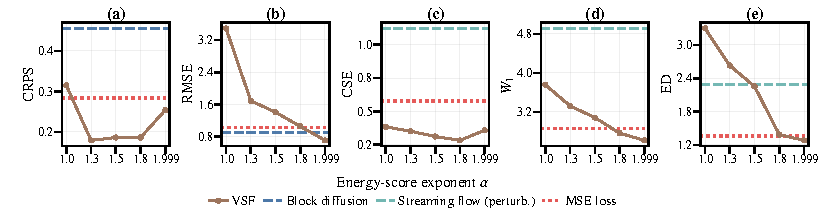
\includegraphics[width=\linewidth]{figures/ablation_plots/combined/crps_beta.pdf}
  \caption{\textbf{Energy-score exponent.} $\alpha$ ablation on (a)--(b)
  deterministic double pendulum and (c)--(e) stochastic R\"ossler. Dashed
  lines show the best overall baseline for each system; dotted lines show
  MSE-trained VSF. Three-seed means.}
  \label{fig:full-ablation-energy-score}
\end{figure}
\end{samepage}

\begin{samepage}
\paragraph{KL regularization.}
Figure~\ref{fig:full-ablation-kl} shows that performance is relatively robust
across the tested KL weights and remains better overall than SF, with an
intermediate weight giving the strongest aggregate result. The KL penalty must
balance retaining target-specific branch information in the training posterior
against aligning that posterior with the prior used for forecasting. When
regularization is too weak $(\beta_{\mathrm{KL}}=1e^{-3})$, the posterior--prior gap makes prior samples less
reliable at inference.

\begin{figure}[H]
  \centering
  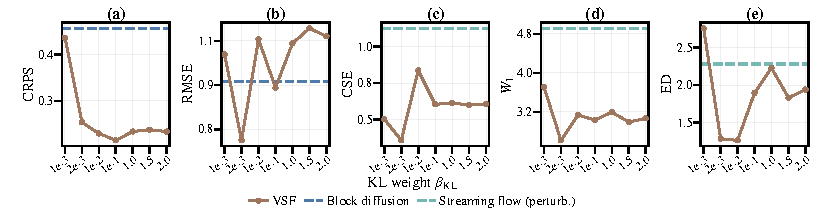
\includegraphics[width=\linewidth]{figures/ablation_plots/combined/kl_beta.pdf}
  \caption{\textbf{KL regularization.} $\beta_{\mathrm{KL}}$ ablation on
  (a)--(b) deterministic double pendulum and (c)--(e) stochastic R\"ossler.
  Dashed lines show the best overall baseline for each system. Three-seed means.}
  \label{fig:full-ablation-kl}
\end{figure}
\end{samepage}

\clearpage
\begin{samepage}
\paragraph{Latent contribution.}
Figure~\ref{fig:full-ablation-latent-weight} varies the latent contribution in
bottleneck-sum fusion. With no latent contribution, the model reduces to SF
and must rely on its evolving predicted history, so rollout errors can
accumulate. Every positive latent contribution improves overall performance
relative to SF by supplying a stable trajectory-level signal that is not
corrupted by previous prediction errors. An intermediate contribution performs
best, indicating that feedback through the recurrent bottleneck remains useful.
Although performance weakens at maximal latent contribution, the model still
retains state and physical-time conditioning and therefore remains robust;
maximal latent contribution does not make the predictor independent of the
physical state.

\begin{figure}[H]
  \centering
  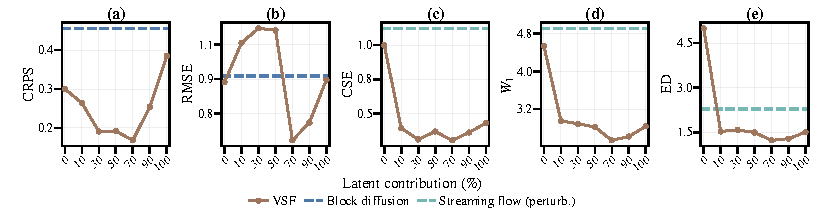
\includegraphics[width=\linewidth]{figures/ablation_plots/combined/latent_weight.pdf}
  \caption{\textbf{Latent contribution.} Bottleneck latent-weight ablation
  on (a)--(b) deterministic double pendulum and (c)--(e) stochastic R\"ossler.
  Dashed lines show the best overall baseline for each system. Three-seed means.}
  \label{fig:full-ablation-latent-weight}
\end{figure}
\end{samepage}

\begin{samepage}
\paragraph{Latent resampling.}
Figure~\ref{fig:full-ablation-resampling} compares sampling one latent for the
complete rollout with drawing a new latent at every forecast step. The two
strategies perform similarly early in the forecast, but the gap widens with
horizon in favor of a fixed latent. A rollout-wise fixed $\vz$ provides a
coherent trajectory-level source of uncertainty, whereas stepwise resampling
introduces temporally inconsistent perturbations and primarily harms
long-horizon probabilistic accuracy.

\begin{figure}[H]
  \centering
  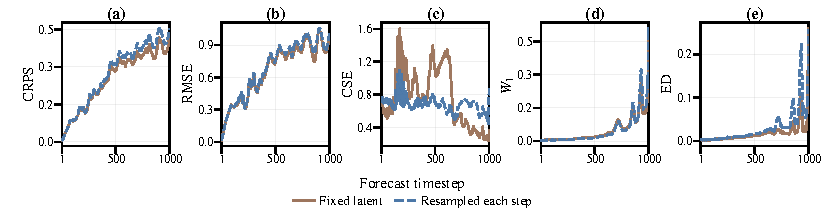
\includegraphics[width=\linewidth]{figures/ablation_plots/combined/latent_resampling.pdf}
  \caption{\textbf{Latent resampling.} Fixed rollout latent versus per-step
  resampling on (a)--(b) deterministic double pendulum and (c)--(e) stochastic
  R\"ossler. Three-seed means.}
  \label{fig:full-ablation-resampling}
\end{figure}
\end{samepage}

\clearpage




\begin{table}[t!]
  \centering
  \small
  \setlength{\tabcolsep}{4pt}
  \renewcommand{\arraystretch}{1.08}
  \caption{Definition of the latent-source and prior-alignment variants.}
  \begin{tabular}{@{}lcccc@{}}
    \toprule
    Variant & Training latent & \shortstack{Posterior\\encoder}
    & $\beta_{\mathrm{KL}}$ & Forecast latent \\
    \midrule
    SF & None & No & -- & None \\
    Prior-latent SF
    & $\vz^{(1:M)}\stackrel{\mathrm{iid}}{\sim}p(\vz)$
    & No & -- & $\vz\sim p(\vz)$, fixed \\
    Posterior VSF (no KL)
    & $\vz^{(1:M)}\stackrel{\mathrm{iid}}{\sim}q_{\vphi}$
    & Yes & $0$ & $\vz\sim p(\vz)$, fixed \\
    Full VSF
    & $\vz^{(1:M)}\stackrel{\mathrm{iid}}{\sim}q_{\vphi}$
    & Yes & $2\times10^{-3}$ & $\vz\sim p(\vz)$, fixed \\
    \bottomrule
  \end{tabular}

  \label{tab:latent-variant-definitions}
\end{table}

\begin{figure}[t!]
  \centering
  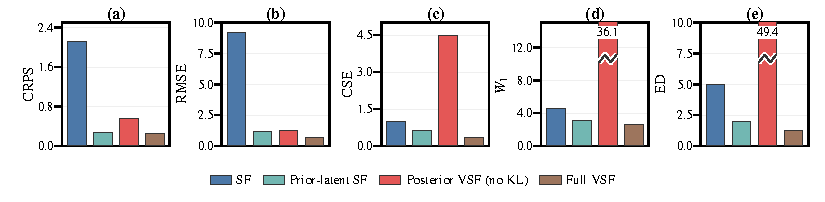
\includegraphics[width=\linewidth]{figures/ablation_plots/combined/latent_prior_alignment.pdf}
  \caption{\textbf{Latent source and prior alignment.} SF, Prior-latent SF,
  Posterior no-KL, and Full VSF on (a)--(b) deterministic double pendulum and
  (c)--(e) stochastic R\"ossler. Three-seed means; breaks mark labeled
  out-of-range values.}
  \label{fig:latent-prior-alignment-ablation}
\end{figure}


\paragraph{Latent-source and prior-alignment variants.}Figure~\ref{fig:latent-prior-alignment-ablation} separates three effects that
are otherwise coupled in VSF: stochastic latent conditioning,
future-conditioned variational training, and alignment of the training
posterior with the inference prior. Here
$p(\vz)=\mathcal N(\mathbf 0,\mathbf I_{d_z})$, and
$q_{\vphi}:=q_{\vphi}(\vz\mid\vu_s,\vx_s,s,\vh)$ is the
future-conditioned training posterior. Table~\ref{tab:latent-variant-definitions}
defines the four variants explicitly.

SF is the non-latent, MSE-trained reference. The three latent-conditioned
variants use the same decoder, $M$-sample generalized energy reconstruction
loss, and bottleneck latent contribution of $0.9$. Prior-latent SF is the
direct non-variational control: it uses prior samples during both training and
forecasting, with neither a posterior encoder nor a KL loss. In contrast,
Posterior VSF (no KL) remains variational because it uses the
future-conditioned posterior during training. Its prior samples at inference
are therefore unaligned with the training latents, creating a train--test
mismatch.

\paragraph{Does latent conditioning help?}
Prior-latent SF versus SF measures the benefit of the latent-conditioned,
multi-sample predictor without a learned posterior. Its improvement across
all  metrics shows that latent-conditioned prediction is already
useful without variational training.

\paragraph{Does variational training help?}
Full VSF has lower error than Prior-latent SF on all five metrics in Figure~\ref{fig:latent-prior-alignment-ablation}. Prior-latent SF samples training latents independently of the motion it must predict, making it harder to associate latent values with different possible futures. Full VSF instead infers latents from the observed local motion during training, helping different latent values represent different continuations. This is useful near a bifurcation, where nearly identical physical states can lead to different outcomes.


\paragraph{Why prior alignment matters.}
Full VSF versus Posterior no-KL isolates the role of the KL term when training
uses a future-conditioned posterior. Removing alignment degrades every metric,
especially the R\"ossler distributional scores. This is consistent with
train--test mismatch. Without KL
regularization, posterior codes may occupy regions or relative masses that are
not reproduced by the prior, so prior-sampled rollouts can miss or misweight
learned continuations. The gains from posterior-based training therefore
depend on aligning it with the forecasting prior.







\clearpage
\section{Rollout Error Plots}
\label{sec:rollout-error-plots}


\begin{figure}[h!]
  \centering
  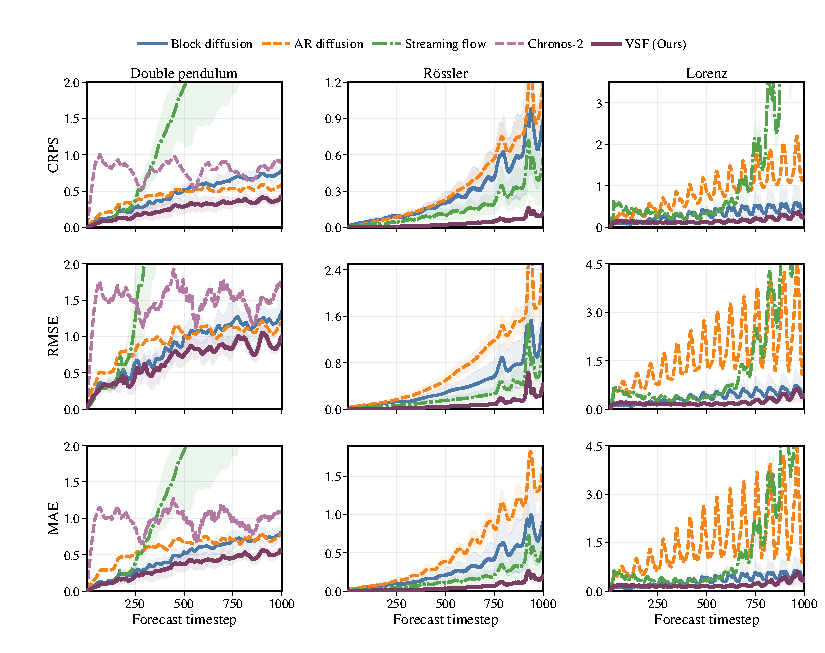
\includegraphics[width=\linewidth]{figures/rollout_error_plots/combined/rollout_errors_deterministic.pdf}
  \caption{Per-timestep error accumulation for 1,000-step deterministic
  forecasts. Columns show double pendulum, R\"ossler, and Lorenz; rows show
  CRPS, RMSE, and MAE. Curves and shaded bands report the mean and one standard
  deviation.}
  \label{fig:rollout-errors-deterministic}
\end{figure}
%  seed 100, 107, and 125

\begin{figure}[h!]
  \centering
  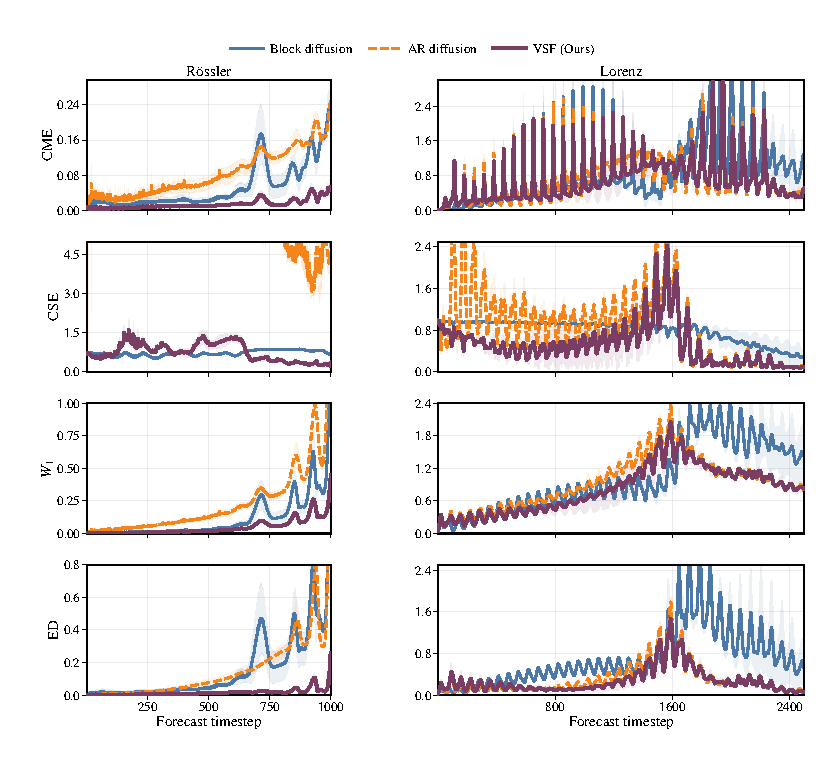
\includegraphics[width=\linewidth]{figures/rollout_error_plots/combined/rollout_errors_stochastic.pdf}
  \caption{Per-timestep distributional error for stochastic R\"ossler over
  1,000 steps and stochastic Lorenz over 2,500 steps. Columns show the two
  systems; rows show CME, CSE, marginal $W_1$, and marginal energy distance.
  Curves and shaded bands report the mean and one standard deviation. These per-timestep scores compare marginal
  standardized state distributions. They provide a different view from the joint whole-trajectory metrics in Table~\ref{tab:forecasting_results}
  and~\ref{tab:stochastic-lorenz-2500}.}
  \label{fig:rollout-errors-stochastic}
\end{figure}




% Select one of the available instances by setting each flag to 01--05.
% Double pendulum uses two independent instances for its two regimes.
% These defaults may also be overridden before this file is input.
\providecommand{\DoublePendulumInstance}{01}
\providecommand{\DoublePendulumChaoticInstance}{02}
\providecommand{\DeterministicRosslerInstance}{01}
\providecommand{\DeterministicLorenzInstance}{01}
\providecommand{\StochasticRosslerInstance}{01}
\providecommand{\StochasticLorenzInstance}{01}

% Select five of the ten exported stochastic-Lorenz draws (01--10).
% Each selector is applied consistently to GT and every forecasting method.
\providecommand{\StochasticLorenzDrawOne}{01}
\providecommand{\StochasticLorenzDrawTwo}{08}
\providecommand{\StochasticLorenzDrawThree}{03}
\providecommand{\StochasticLorenzDrawFour}{04}
\providecommand{\StochasticLorenzDrawFive}{05}
\providecommand{\StochasticLorenzDrawSix}{06}
\providecommand{\StochasticLorenzDrawSeven}{07}



\newlength{\qualpanelwidth}
\newlength{\qualpanelheight}
\setlength{\qualpanelwidth}{0.225\linewidth}
\setlength{\qualpanelheight}{0.215\linewidth}
\newcommand{\qualplaceholder}{%
  \fbox{\parbox[c][\dimexpr\qualpanelheight-2\fboxsep-2\fboxrule\relax][c]{%
    \dimexpr\qualpanelwidth-2\fboxsep-2\fboxrule\relax}{%
    \centering\scriptsize Image\\placeholder}}%
}
\newcommand{\qualgraphic}[1]{%
  \includegraphics[
    width=\qualpanelwidth,
    height=\qualpanelheight,
    keepaspectratio
  ]{#1}%
}
\newcommand{\qualpanel}[1]{%
  \IfFileExists{#1.pdf}{%
    \qualgraphic{#1.pdf}%
  }{%
    \IfFileExists{#1.png}{\qualgraphic{#1.png}}{\qualplaceholder}%
  }%
}
\newcommand{\quallabelfont}{\normalfont\small}
\newcommand{\qualheader}[1]{{\quallabelfont\shortstack{#1}}}
\newcommand{\qualrowlabel}[1]{%
  \parbox[b][\qualpanelheight][c]{2em}{%
    \centering
    \rotatebox[origin=c]{90}{{\quallabelfont\shortstack{#1}}}%
  }%
}
\newcommand{\qualdeterministicrow}[2]{%
  \qualrowlabel{#1}
  & \qualpanel{#2_samples_gt}
  & \qualpanel{#2_samples_vsf}
  & \qualpanel{#2_mean_vsf}
  & \qualpanel{#2_samples_streaming_flow}
  & \qualpanel{#2_samples_block_diffusion} \\[0.2em]
}
\newcommand{\qualzoomrow}[2]{%
  \qualrowlabel{#1}
  & \multicolumn{5}{c}{%
    \parbox[b][\qualpanelheight][c]{%
      \dimexpr5\qualpanelwidth+8\tabcolsep\relax}{%
      \centering
      \includegraphics[
        width=\linewidth,
        height=\qualpanelheight,
        keepaspectratio
      ]{#2}%
    }%
  } \\[0.2em]
}

\newcommand{\stochasticlorenzrow}[2]{%
  {\quallabelfont #1}
  & \qualpanel{figures/lorenz_stochastic/instance_\StochasticLorenzInstance%
      _stochastic_lorenz_draw_#2_gt}
  & \qualpanel{figures/lorenz_stochastic/instance_\StochasticLorenzInstance%
      _stochastic_lorenz_draw_#2_vsf}
  & \qualpanel{figures/lorenz_stochastic/instance_\StochasticLorenzInstance%
      _stochastic_lorenz_draw_#2_streaming_flow}
  & \qualpanel{figures/lorenz_stochastic/instance_\StochasticLorenzInstance%
      _stochastic_lorenz_draw_#2_block_diffusion}
  & \qualpanel{figures/lorenz_stochastic/instance_\StochasticLorenzInstance%
      _stochastic_lorenz_draw_#2_ar_diffusion} \\[0.15em]
}


\clearpage
\section{Trajectory Forecast Visualizations}
\label{sec:qualitative-trajectory-forecasts}
We compare sampled forecast trajectories across the evaluated systems and
baselines. For the deterministic systems, we additionally show the VSF
ensemble predictive mean.

\begin{figure}[h!]
  \centering
  \begingroup
  \setlength{\qualpanelwidth}{0.18\linewidth}
  \setlength{\qualpanelheight}{0.18\linewidth}
  \setlength{\tabcolsep}{0.75pt}
  \renewcommand{\arraystretch}{1.0}
  \begin{tabular}{@{}c*{5}{c}@{}}
    & \qualheader{GT}
    & \qualheader{VSF (Ours)}
    & \qualheader{VSF ensemble}
    & \qualheader{SF}
    & \qualheader{Block diffusion} \\[0.15em]
    \qualdeterministicrow{Double \\pendulum}{figures/double_pendulum/instance_%
      \DoublePendulumInstance_deterministic_double_pendulum}
    \qualzoomrow{Double\\pendulum}{figures/zoom_double_pendulum.pdf}
    \qualzoomrow{R\"ossler}{figures/zoom_deterministic_rossler.pdf}
    \qualzoomrow{Lorenz}{figures/zoom_deterministic_lorenz.pdf}
  \end{tabular}
  \endgroup
  \caption{Qualitative forecasts on the deterministic systems. Columns show
  ground truth (GT), VSF samples, the VSF ensemble predictive mean, SF, and
  block diffusion. Sample panels contain $N=10$ trajectories; the VSF ensemble is the mean of the samples. The last three rows magnify highlighted regions of the chaotic double-pendulum, R\"ossler, and Lorenz forecasts.}
  \label{fig:qualitative-deterministic}
  \label{fig:main-chaotic-double-pendulum}
  \label{fig:qualitative-deterministic-double-pendulum-chaotic}
  \label{fig:qualitative-deterministic-rossler}
  \label{fig:qualitative-deterministic-lorenz}
\end{figure}

\begin{figure}[h!]
  \centering
  \begingroup
  \setlength{\qualpanelwidth}{0.18\linewidth}
  \setlength{\qualpanelheight}{0.17\linewidth}
  \setlength{\tabcolsep}{1pt}
  \renewcommand{\arraystretch}{1.05}
  \begin{tabular}{@{}c*{5}{c}@{}}
    \qualheader{Sample}
    & \qualheader{GT}
    & \qualheader{VSF (Ours)}
    & \qualheader{SF}
    & \qualheader{Block\\diffusion}
    & \qualheader{AR\\diffusion} \\
    \stochasticlorenzrow{1}{\StochasticLorenzDrawOne}
    \stochasticlorenzrow{2}{\StochasticLorenzDrawTwo}
    \stochasticlorenzrow{3}{\StochasticLorenzDrawThree}
    \stochasticlorenzrow{4}{\StochasticLorenzDrawFour}
    \stochasticlorenzrow{5}{\StochasticLorenzDrawSeven}
  \end{tabular}
  \endgroup
  \caption{Visualization samples from the ground truth and generated trajectories for the partially observed stochastic Lorenz.}
  \label{fig:qualitative-stochastic-lorenz}
\end{figure}



% \clearpage
% \section{World-Model Latent-Trajectory Visualizations}
% \label{sec:world-model-latent-trajectory-visualizations}

% \begin{figure}[H]
%   \centering
%   \begin{tikzpicture}
%     \node[inner sep=0pt,outer sep=0pt] (arp-panel) {%
%       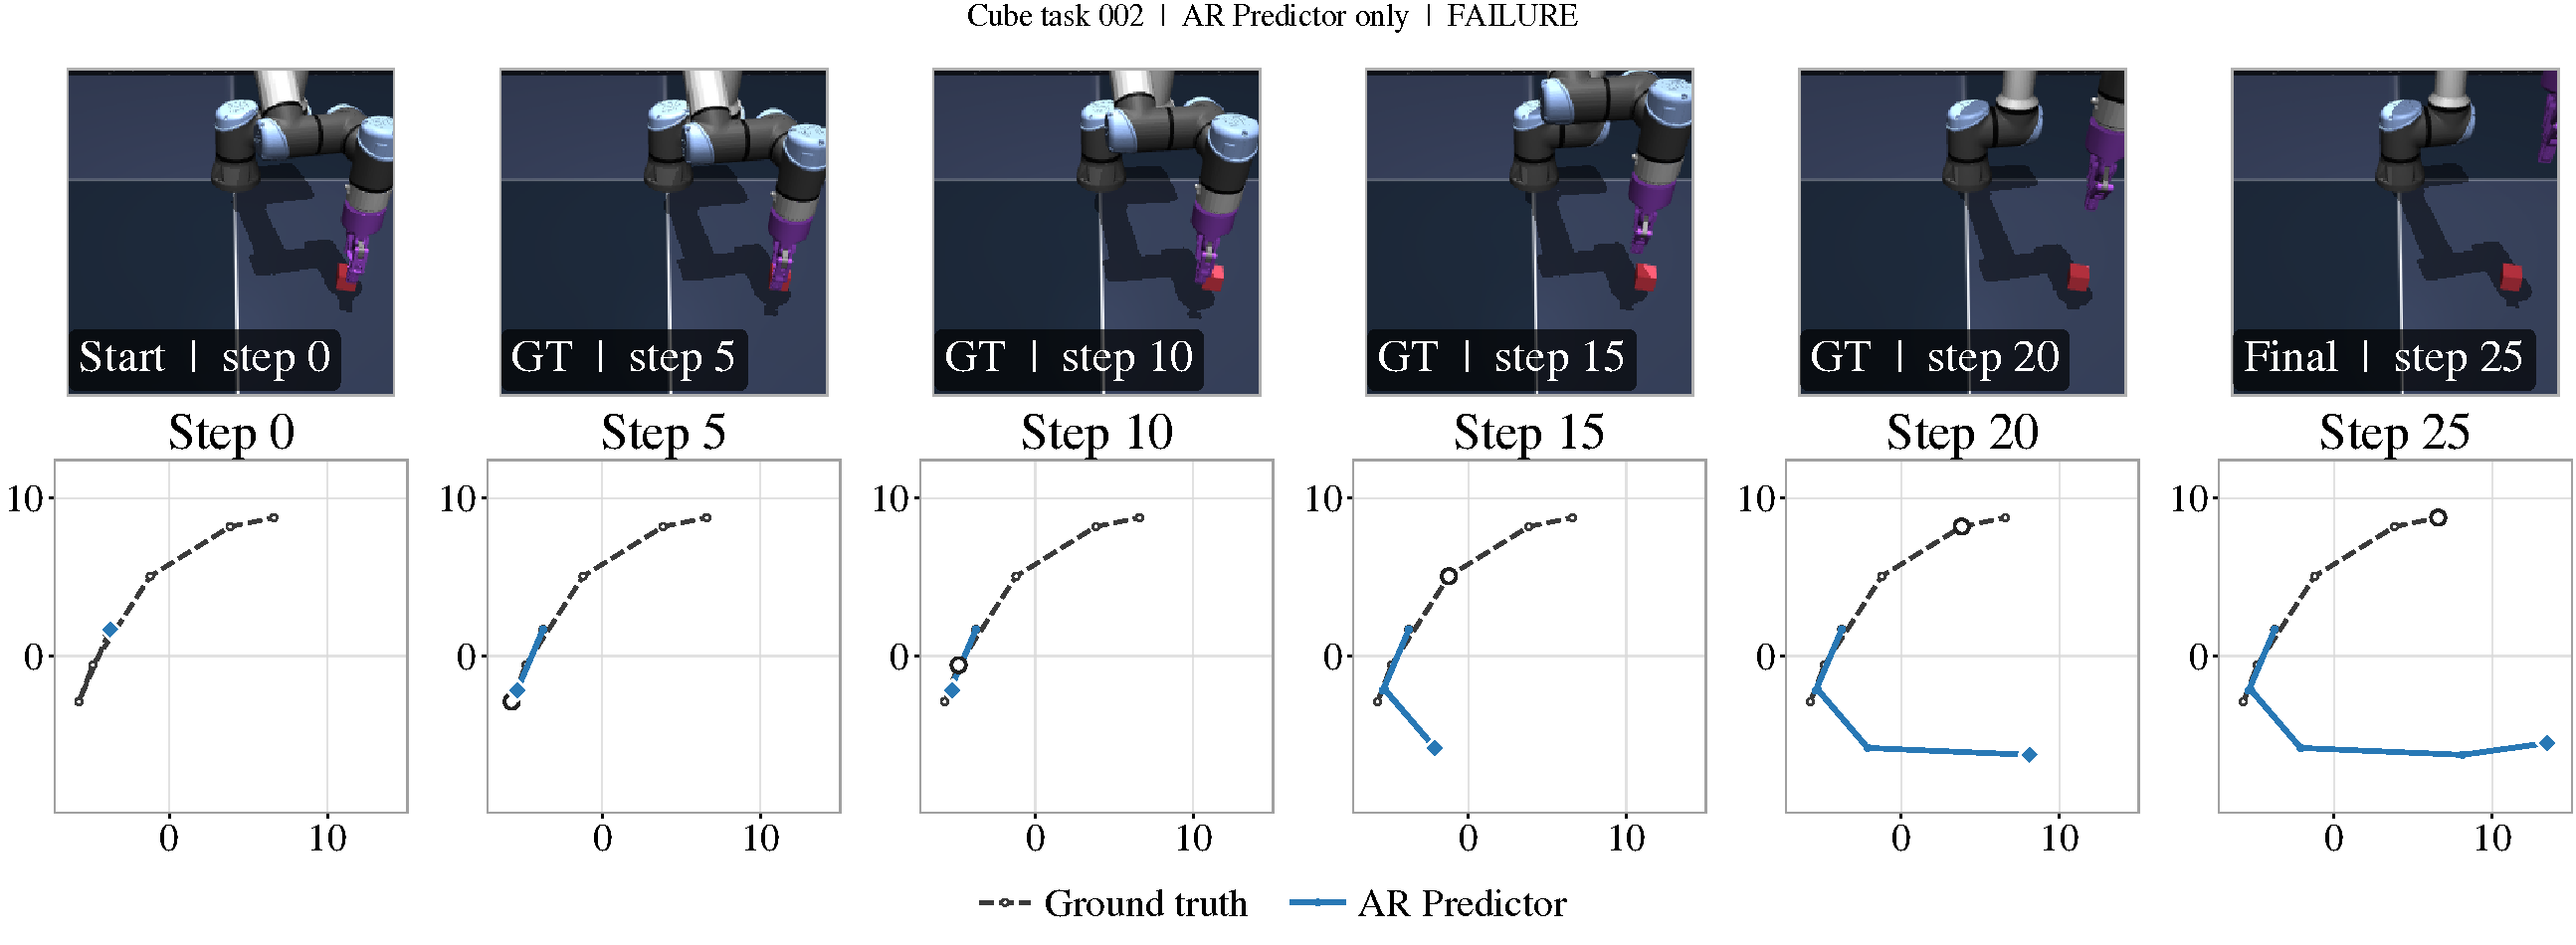
\includegraphics[
%         width=0.78\linewidth,
%         trim={0bp 0bp 0bp 20bp},
%         clip
%       ]{figures/wm/cube_task_002_arp_latent_trajectory.pdf}%
%     };
%     \node[
%       anchor=south west,
%       inner sep=0pt,
%       outer sep=0pt,
%       xshift=0pt,
%       yshift=2pt,
%       font=\normalfont\normalsize
%     ] at (arp-panel.north west) {(a)};
%   \end{tikzpicture}\par\nointerlineskip
%   \begin{tikzpicture}
%     \node[inner sep=0pt,outer sep=0pt] (vsf-panel) {%
%       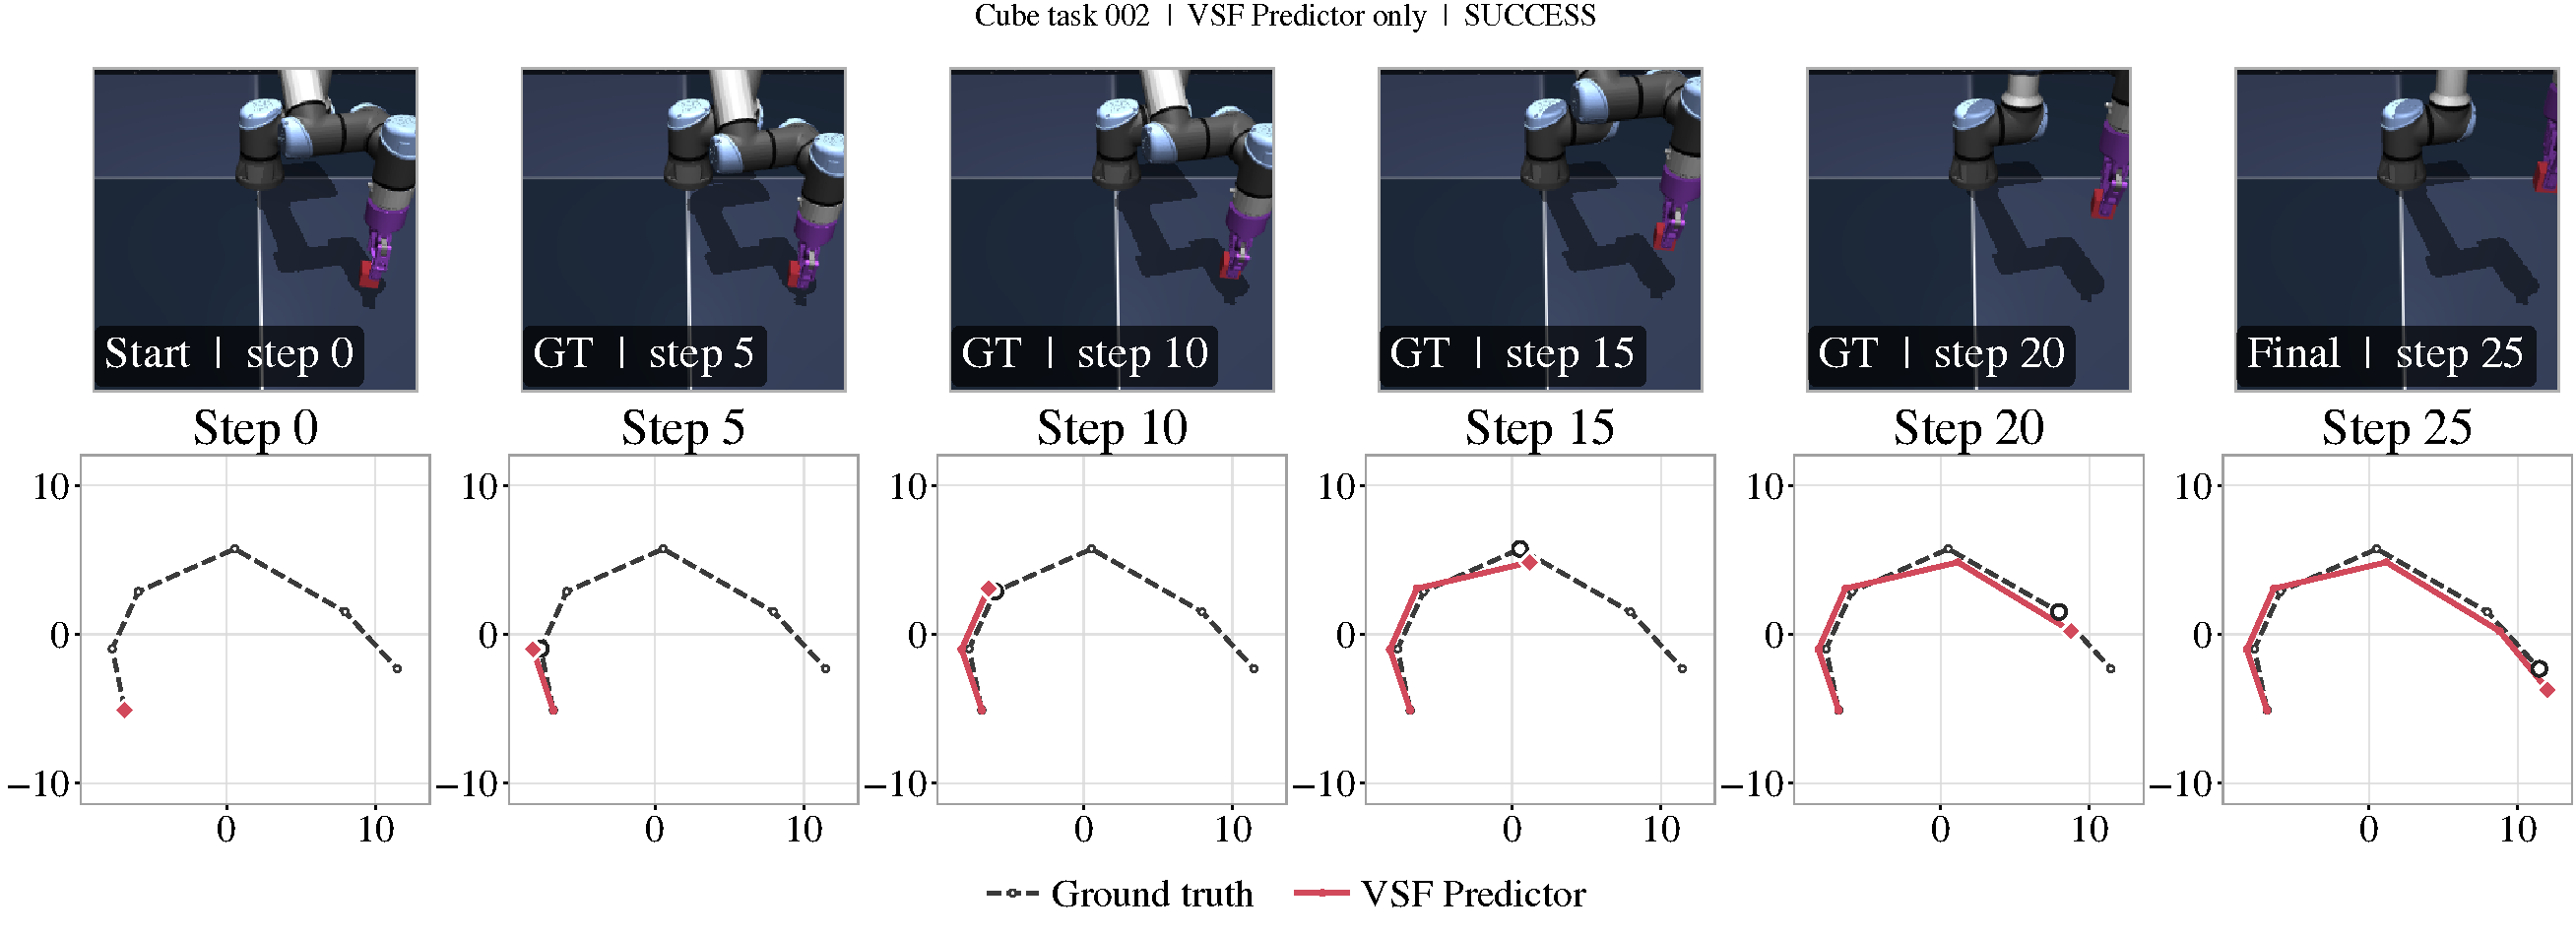
\includegraphics[
%         width=0.78\linewidth,
%         trim={0bp 0bp 0bp 20bp},
%         clip
%       ]{figures/wm/cube_task_002_vsf_latent_trajectory.pdf}%
%     };
%     \node[
%       anchor=south west,
%       inner sep=0pt,
%       outer sep=0pt,
%       xshift=0pt,
%       yshift=2pt,
%       font=\normalfont\normalsize
%     ] at (vsf-panel.north west) {(b)};
%   \end{tikzpicture}
%   \caption{The top row shows the ground-truth observations during rollout. The bottom row compares the predicted and ground-truth latent trajectories after joint-PCA projections. (a) The AR Predictor trajectory diverges
%   and the rollout fails. (b) The VSF Predictor trajectory follows the
%   ground-truth trajectory and the rollout succeeds.}
%   \label{fig:wm-cube-task-002-latent-trajectories}
% \end{figure}

% \begin{figure}[H]
%   \centering
%   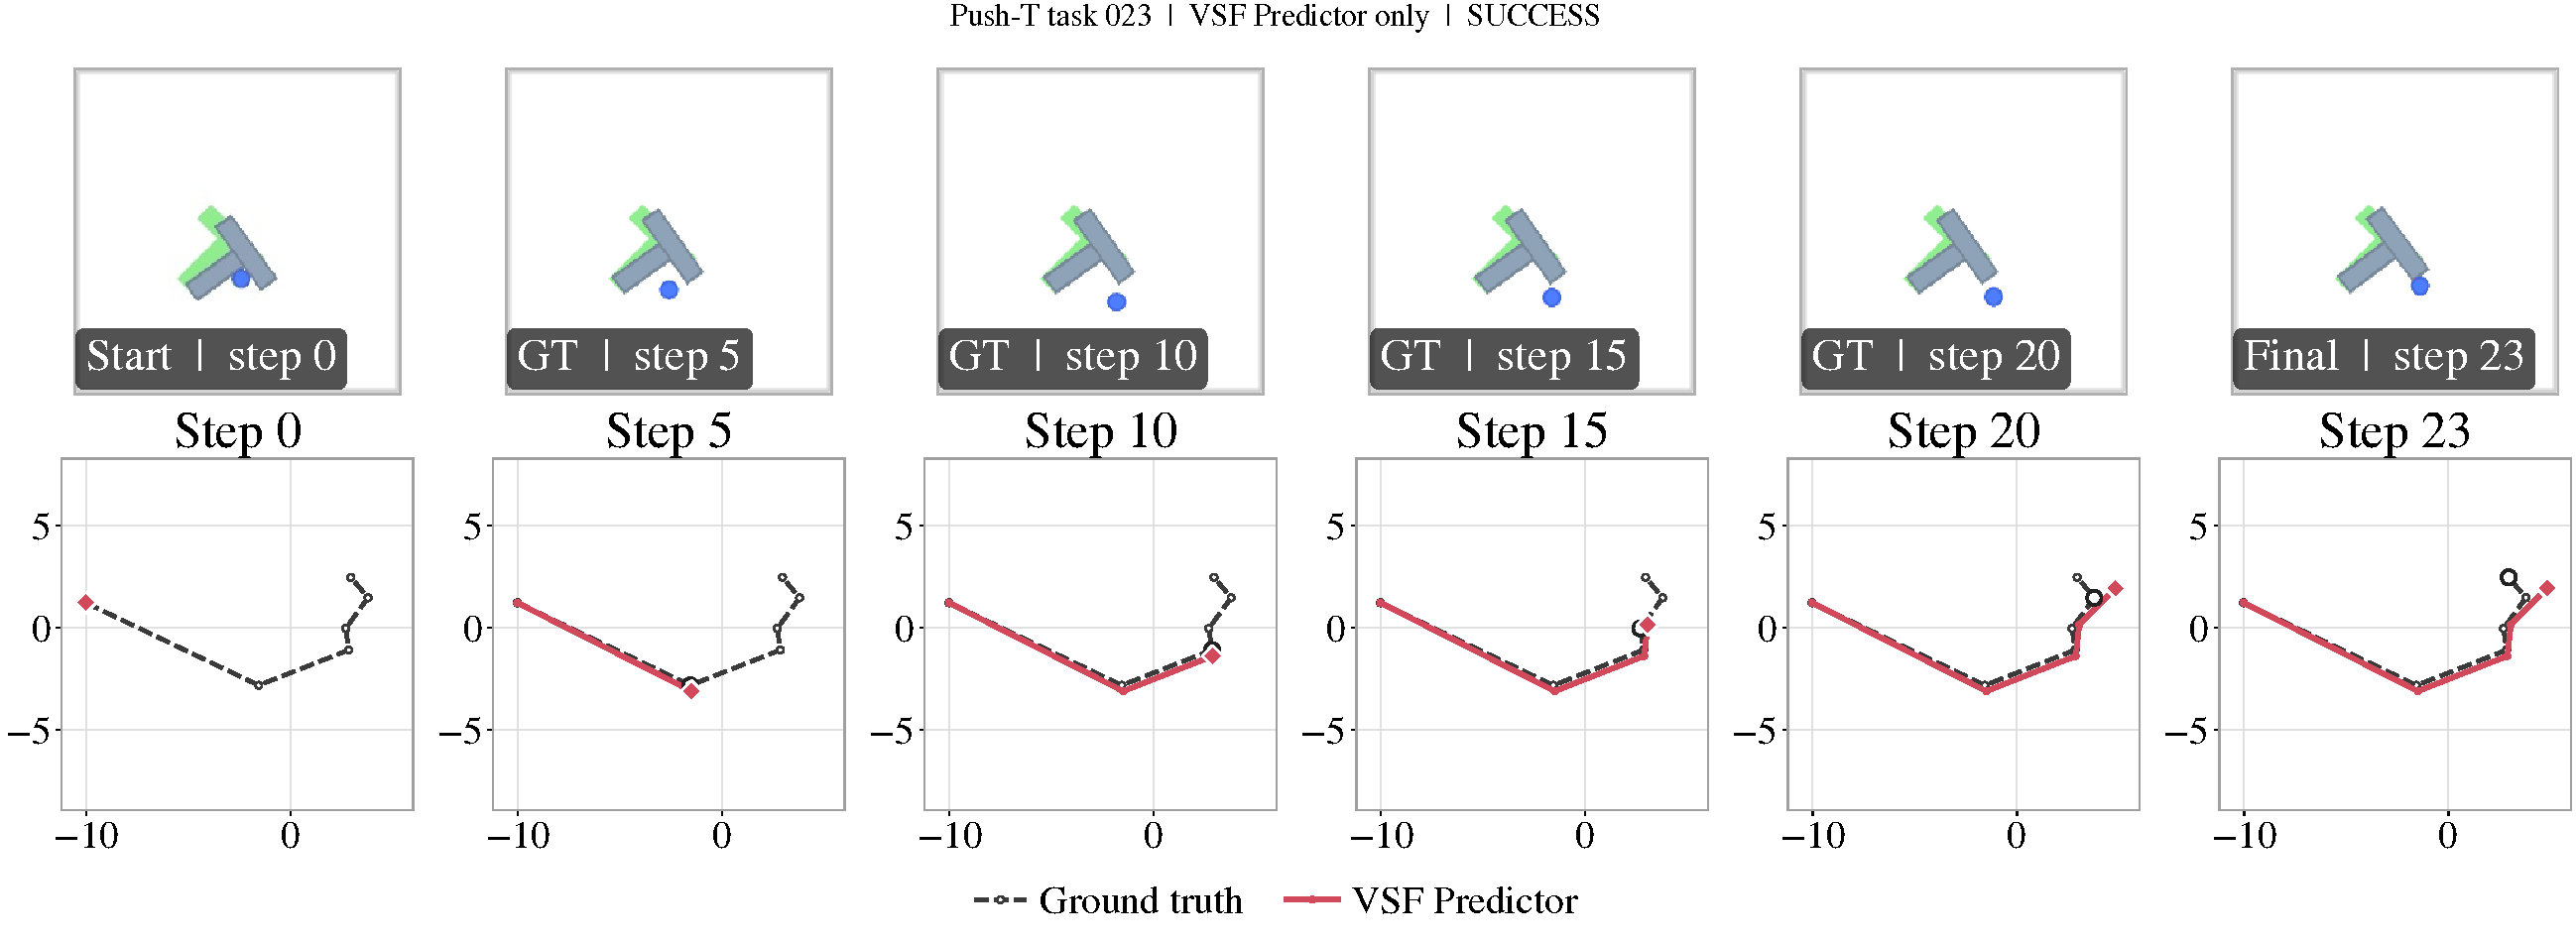
\includegraphics[
%     width=0.78\linewidth,
%     trim={0bp 0bp 0bp 20bp},
%     clip
%   ]{figures/wm/pusht_task_023_vsf_latent_trajectory.pdf}
%   \caption{Qualitative PushT result. VSF action-conditioned predicted latent
%   trajectory follows the ground-truth trajectory in a successful rollout.}
%   \label{fig:wm-vsf-pusht-qualitative}
% \end{figure}

% \begin{figure}[H]
%   \centering
%   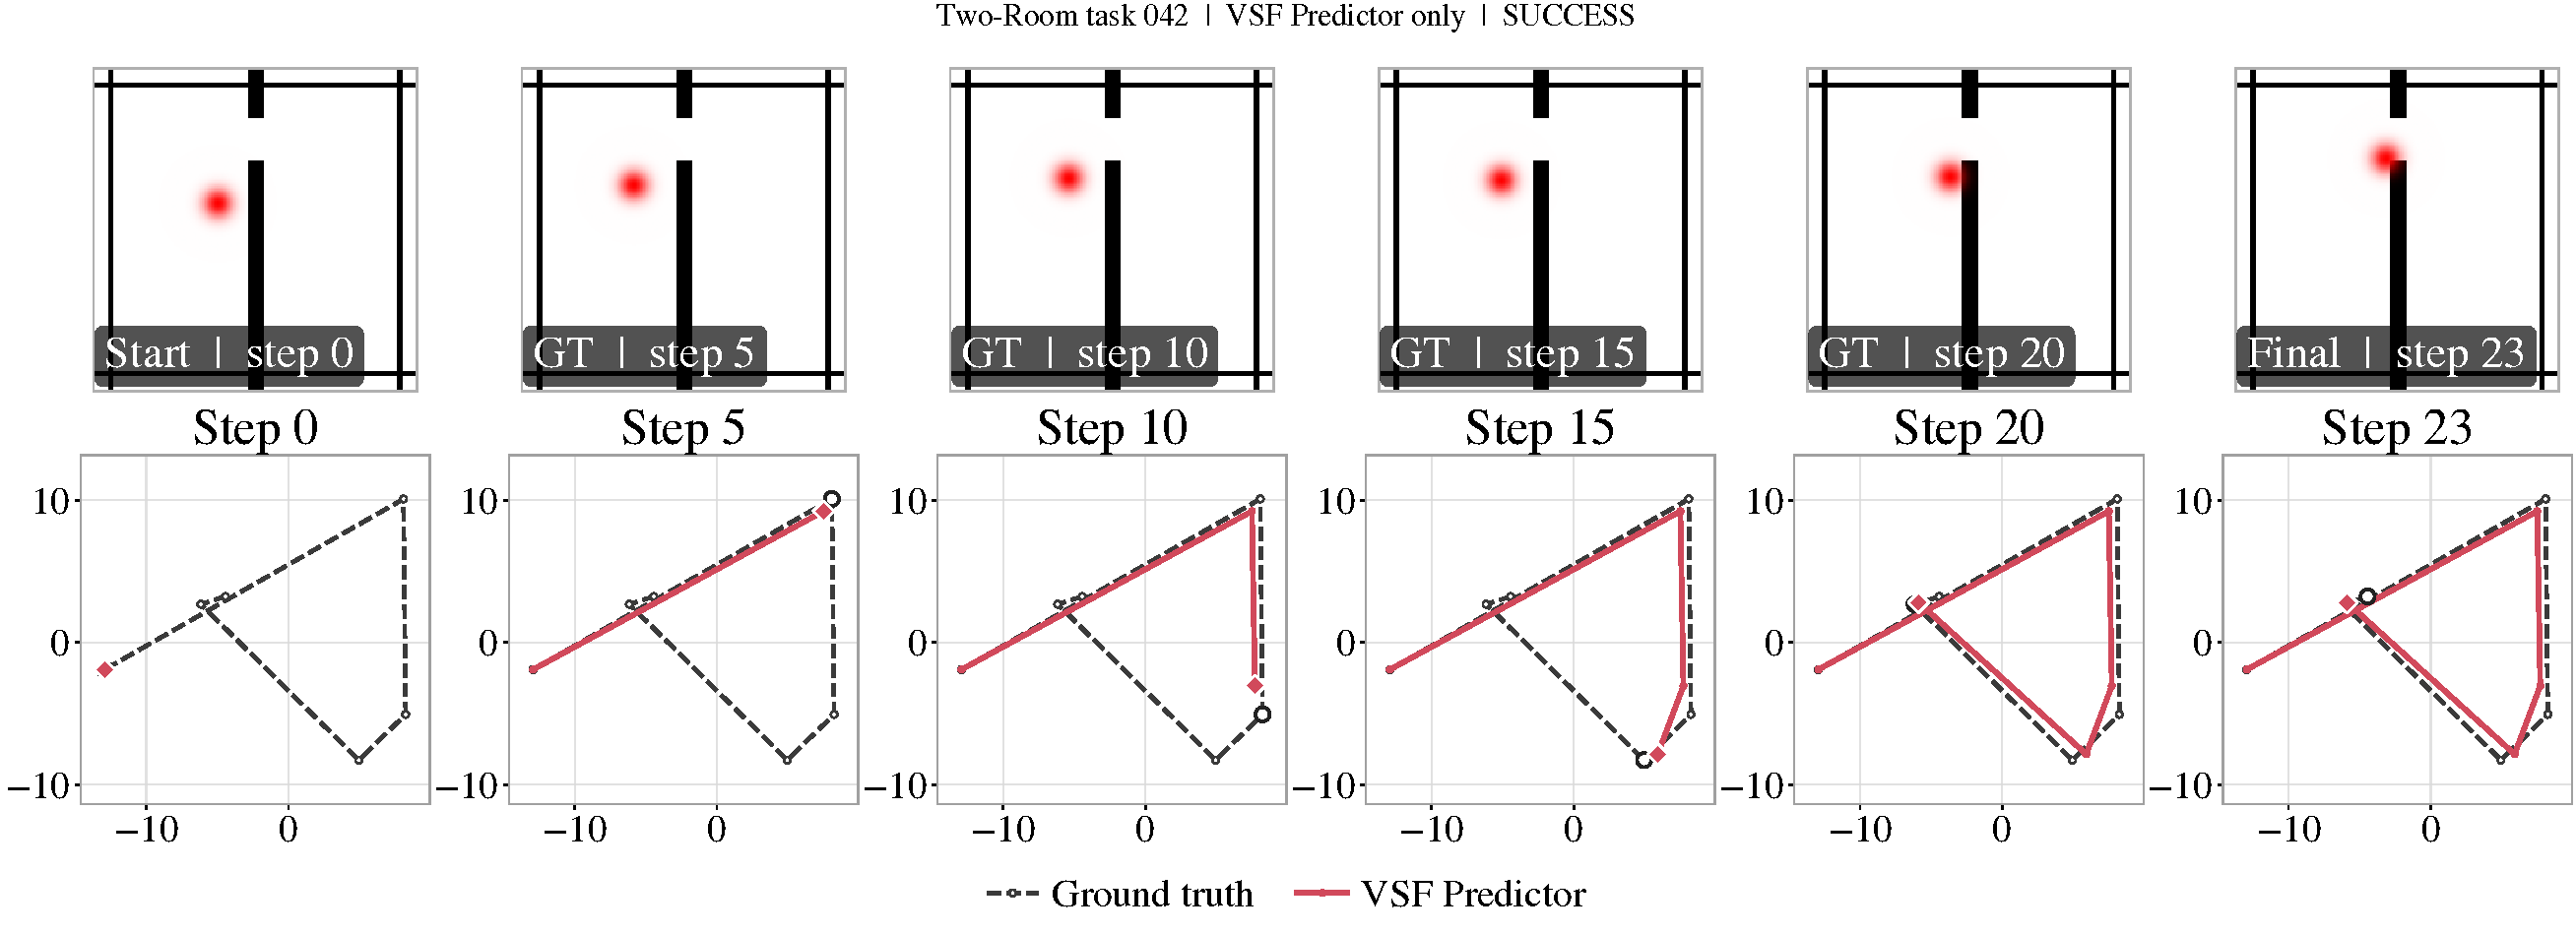
\includegraphics[
%     width=0.78\linewidth,
%     trim={0bp 0bp 0bp 20bp},
%     clip
%   ]{figures/wm/tworoom_task_042_vsf_latent_trajectory.pdf}
%   \caption{Qualitative TwoRoom result. VSF action-conditioned predicted latent
%   trajectory follows the ground-truth trajectory in a successful rollout.}
%   \label{fig:wm-vsf-reacher-qualitative}
% \end{figure}

\clearpage
\section{World-Model Latent-Trajectory Visualizations}
\label{sec:world-model-latent-trajectory-visualizations}

\begin{figure}[H]
  \centering
  \begin{tikzpicture}
    \node[inner sep=0pt,outer sep=0pt] (arp-panel) {%
      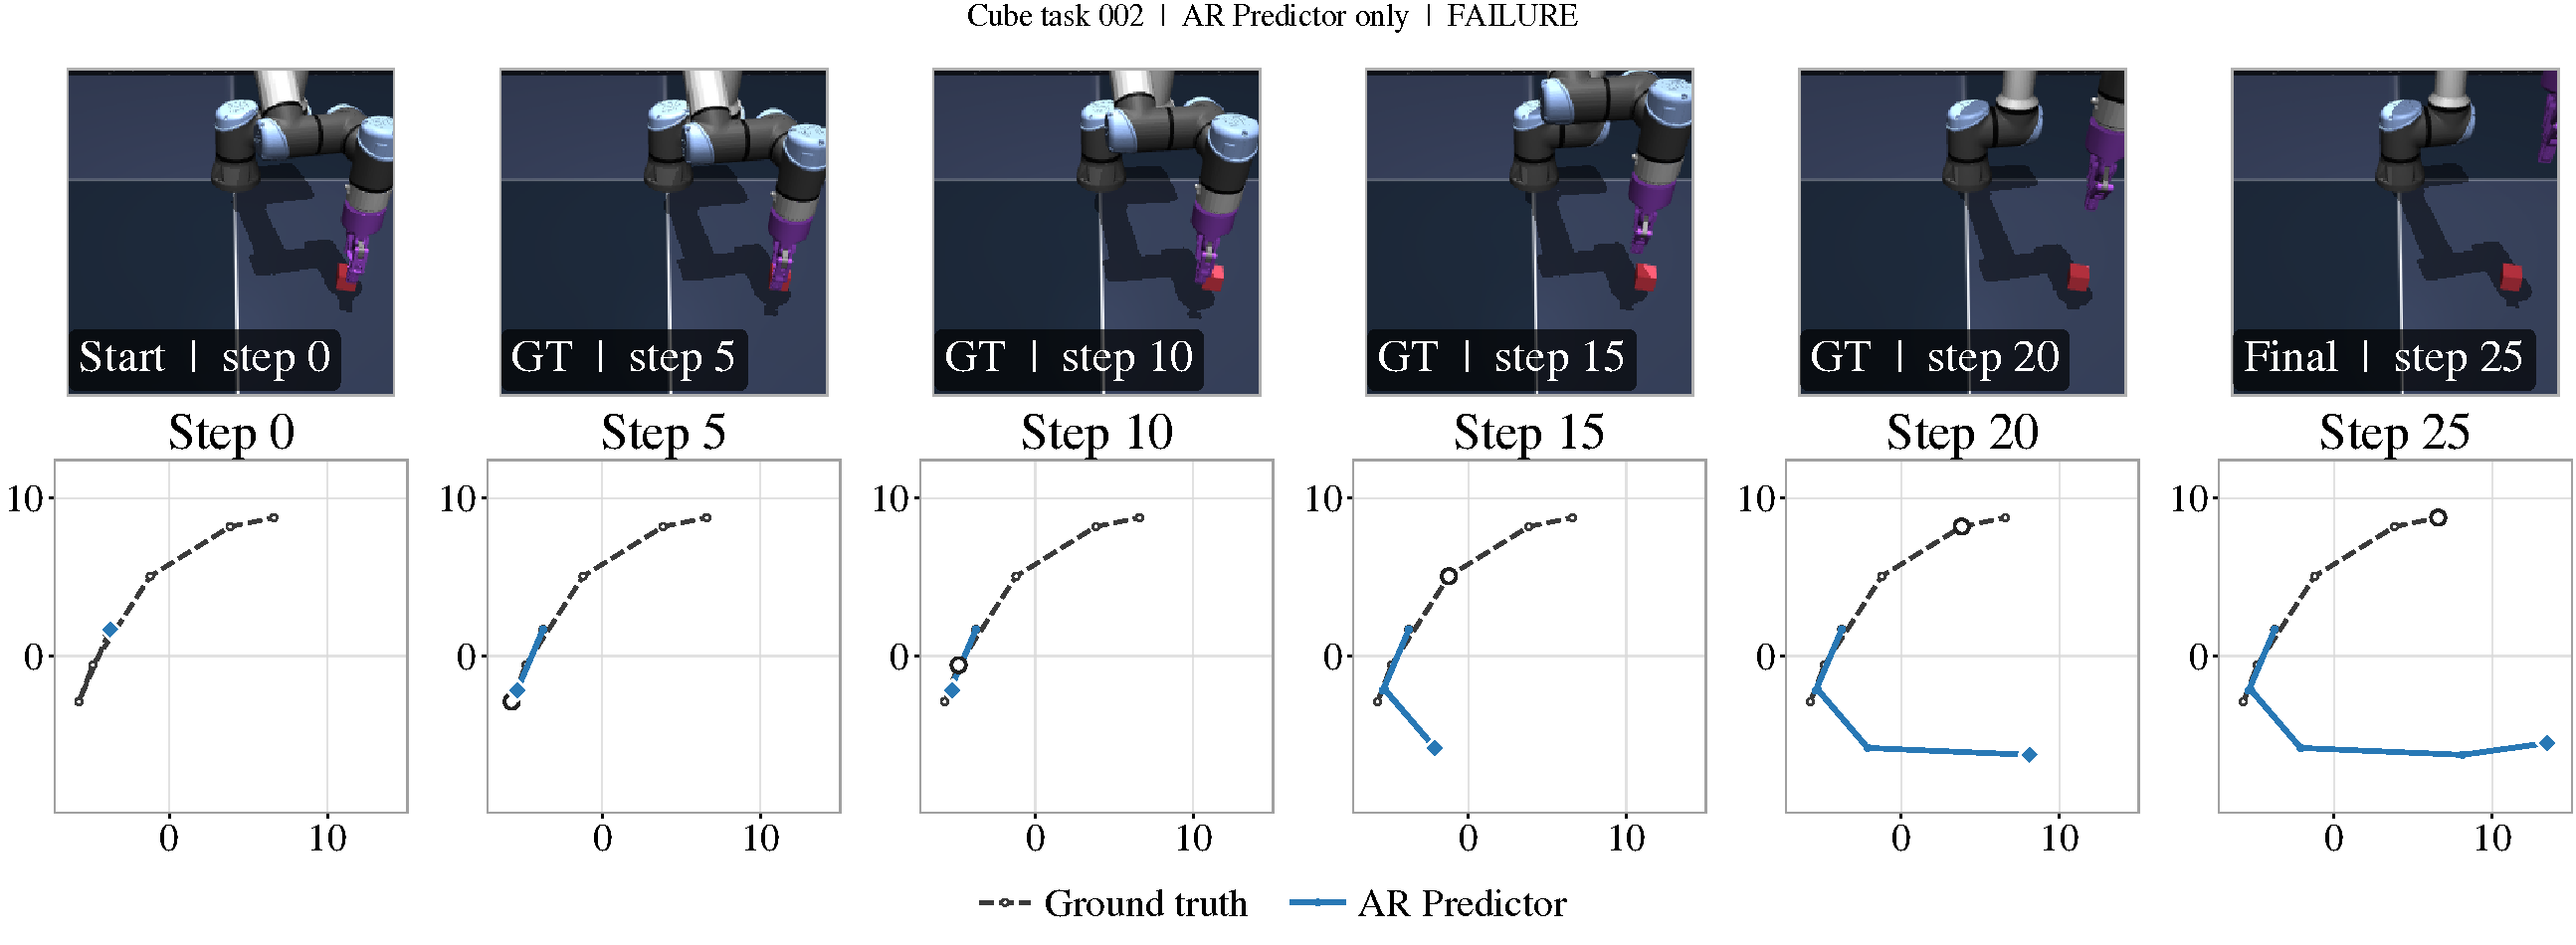
\includegraphics[
        width=\linewidth,
        trim={0bp 0bp 0bp 20bp},
        clip
      ]{figures/wm/cube_task_002_arp_latent_trajectory.pdf}%
    };
    \node[
      anchor=south west,
      inner sep=0pt,
      outer sep=0pt,
      xshift=0pt,
      yshift=2pt,
      font=\normalfont\normalsize
    ] at (arp-panel.north west) {(a)};
  \end{tikzpicture}\par\nointerlineskip
  \begin{tikzpicture}
    \node[inner sep=0pt,outer sep=0pt] (vsf-panel) {%
      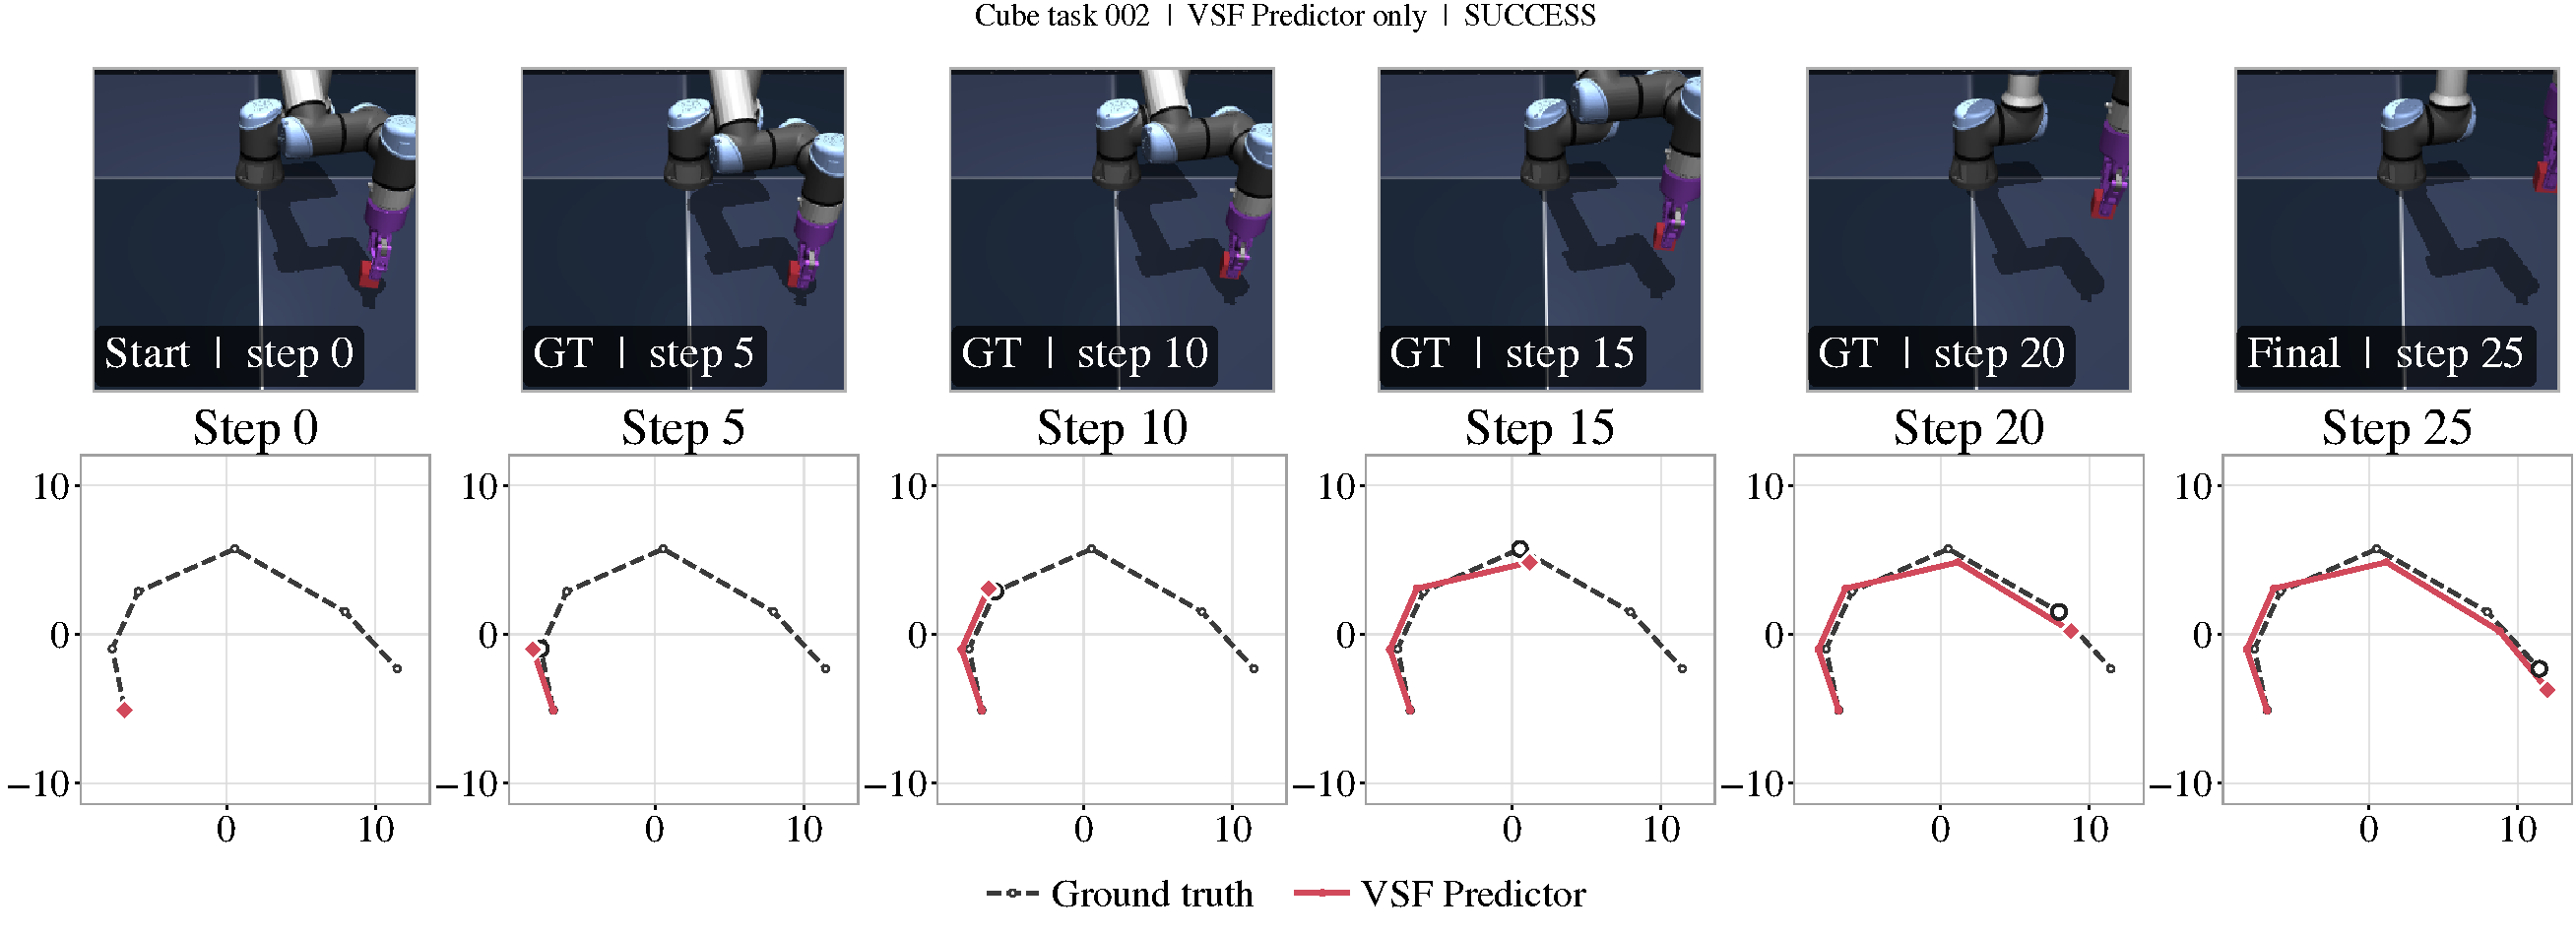
\includegraphics[
        width=\linewidth,
        trim={0bp 0bp 0bp 20bp},
        clip
      ]{figures/wm/cube_task_002_vsf_latent_trajectory.pdf}%
    };
    \node[
      anchor=south west,
      inner sep=0pt,
      outer sep=0pt,
      xshift=0pt,
      yshift=2pt,
      font=\normalfont\normalsize
    ] at (vsf-panel.north west) {(b)};
  \end{tikzpicture}
  \caption{The top row shows the ground-truth observations during rollout. The bottom row compares the predicted and ground-truth latent trajectories after joint-PCA projections. (a) The AR Predictor trajectory diverges
  and the rollout fails. (b) The VSF Predictor trajectory follows the
  ground-truth trajectory and the rollout succeeds.}
  \label{fig:wm-cube-task-002-latent-trajectories}
\end{figure}

\clearpage
\begin{figure}[H]
  \centering
  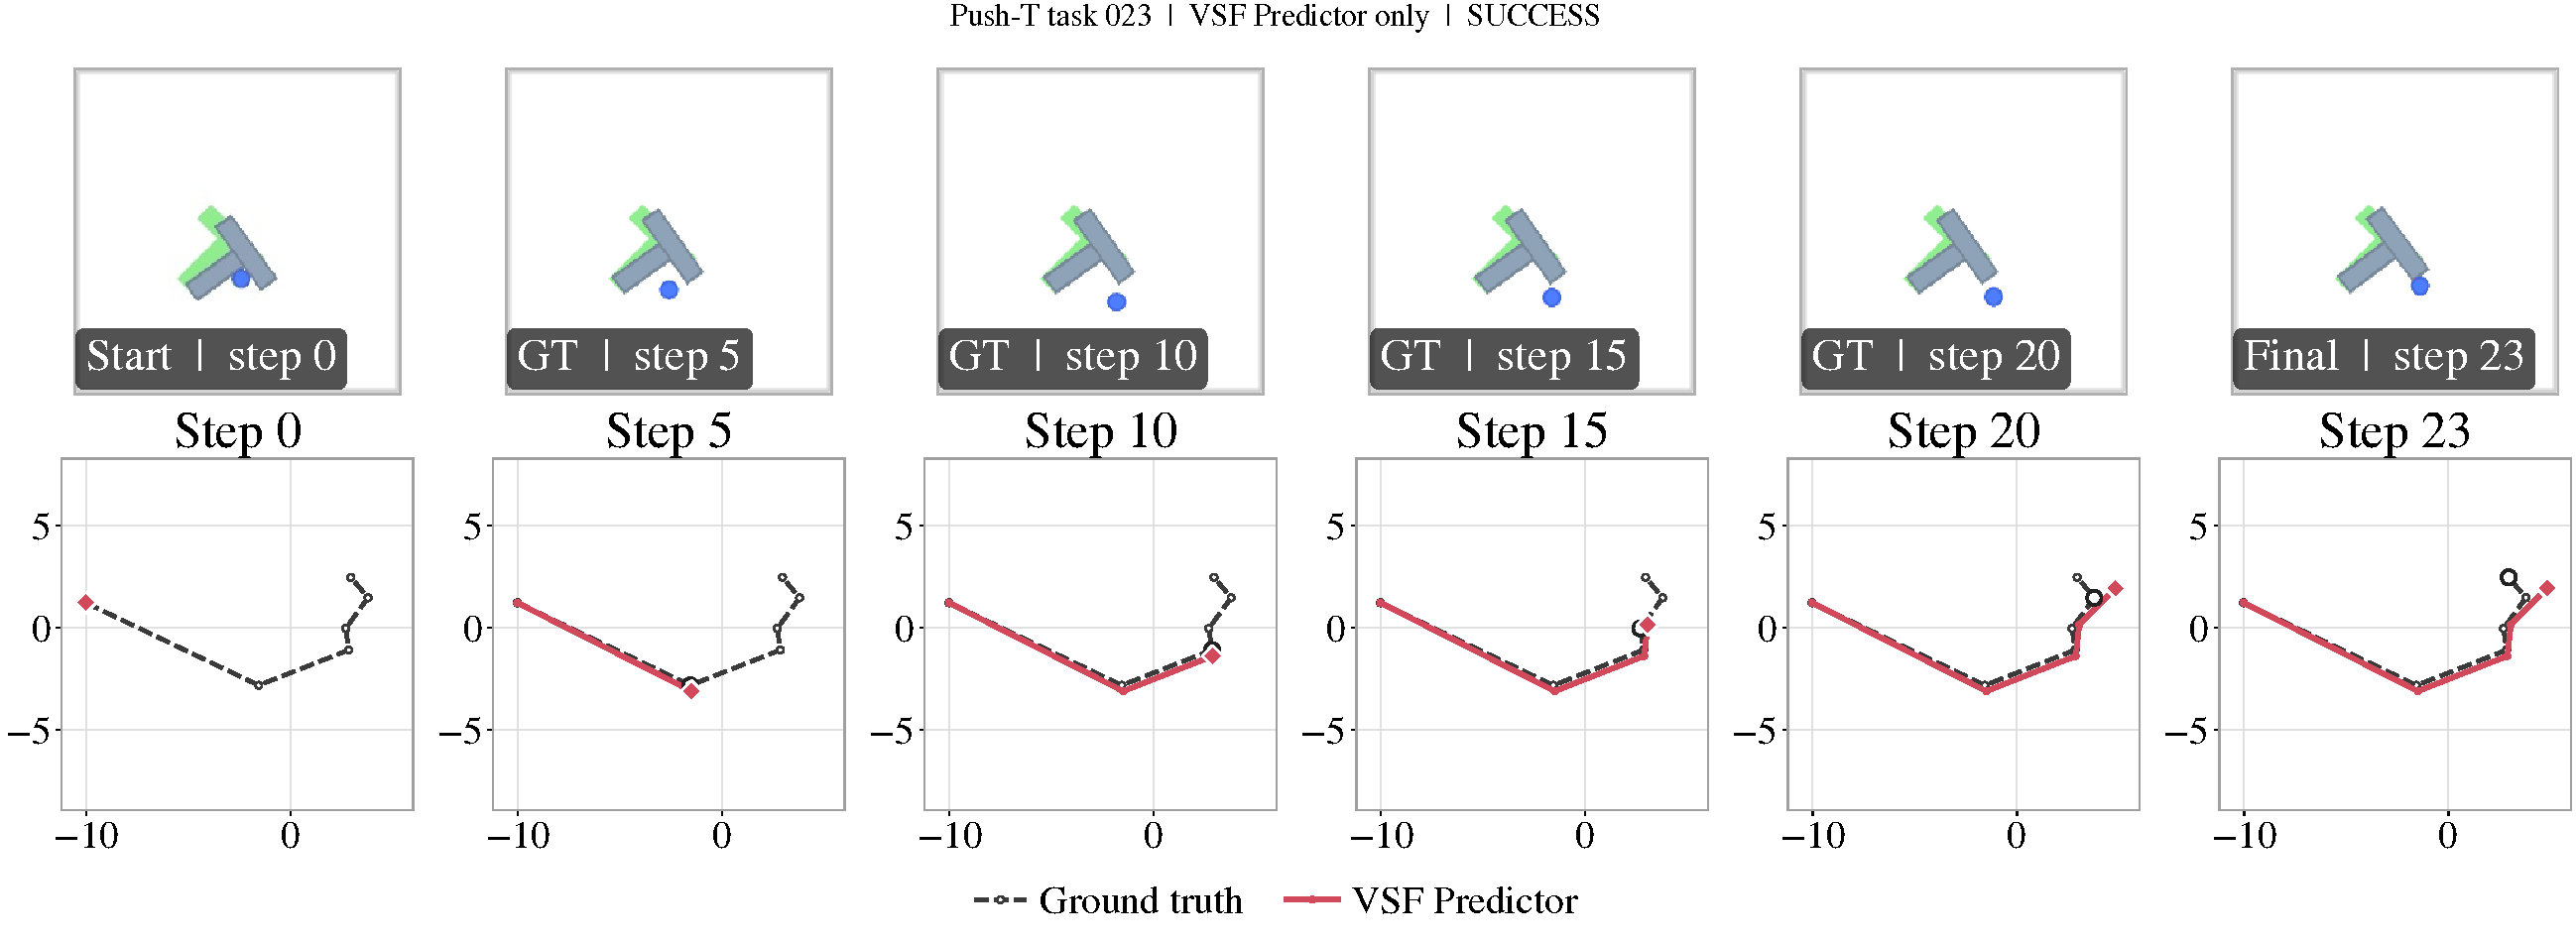
\includegraphics[
    width=\linewidth,
    trim={0bp 0bp 0bp 20bp},
    clip
  ]{figures/wm/pusht_task_023_vsf_latent_trajectory.pdf}
  \caption{Qualitative PushT result. VSF action-conditioned predicted latent
  trajectory follows the ground-truth trajectory in a successful rollout.}
  \label{fig:wm-vsf-pusht-qualitative}
\end{figure}

\begin{figure}[H]
  \centering
  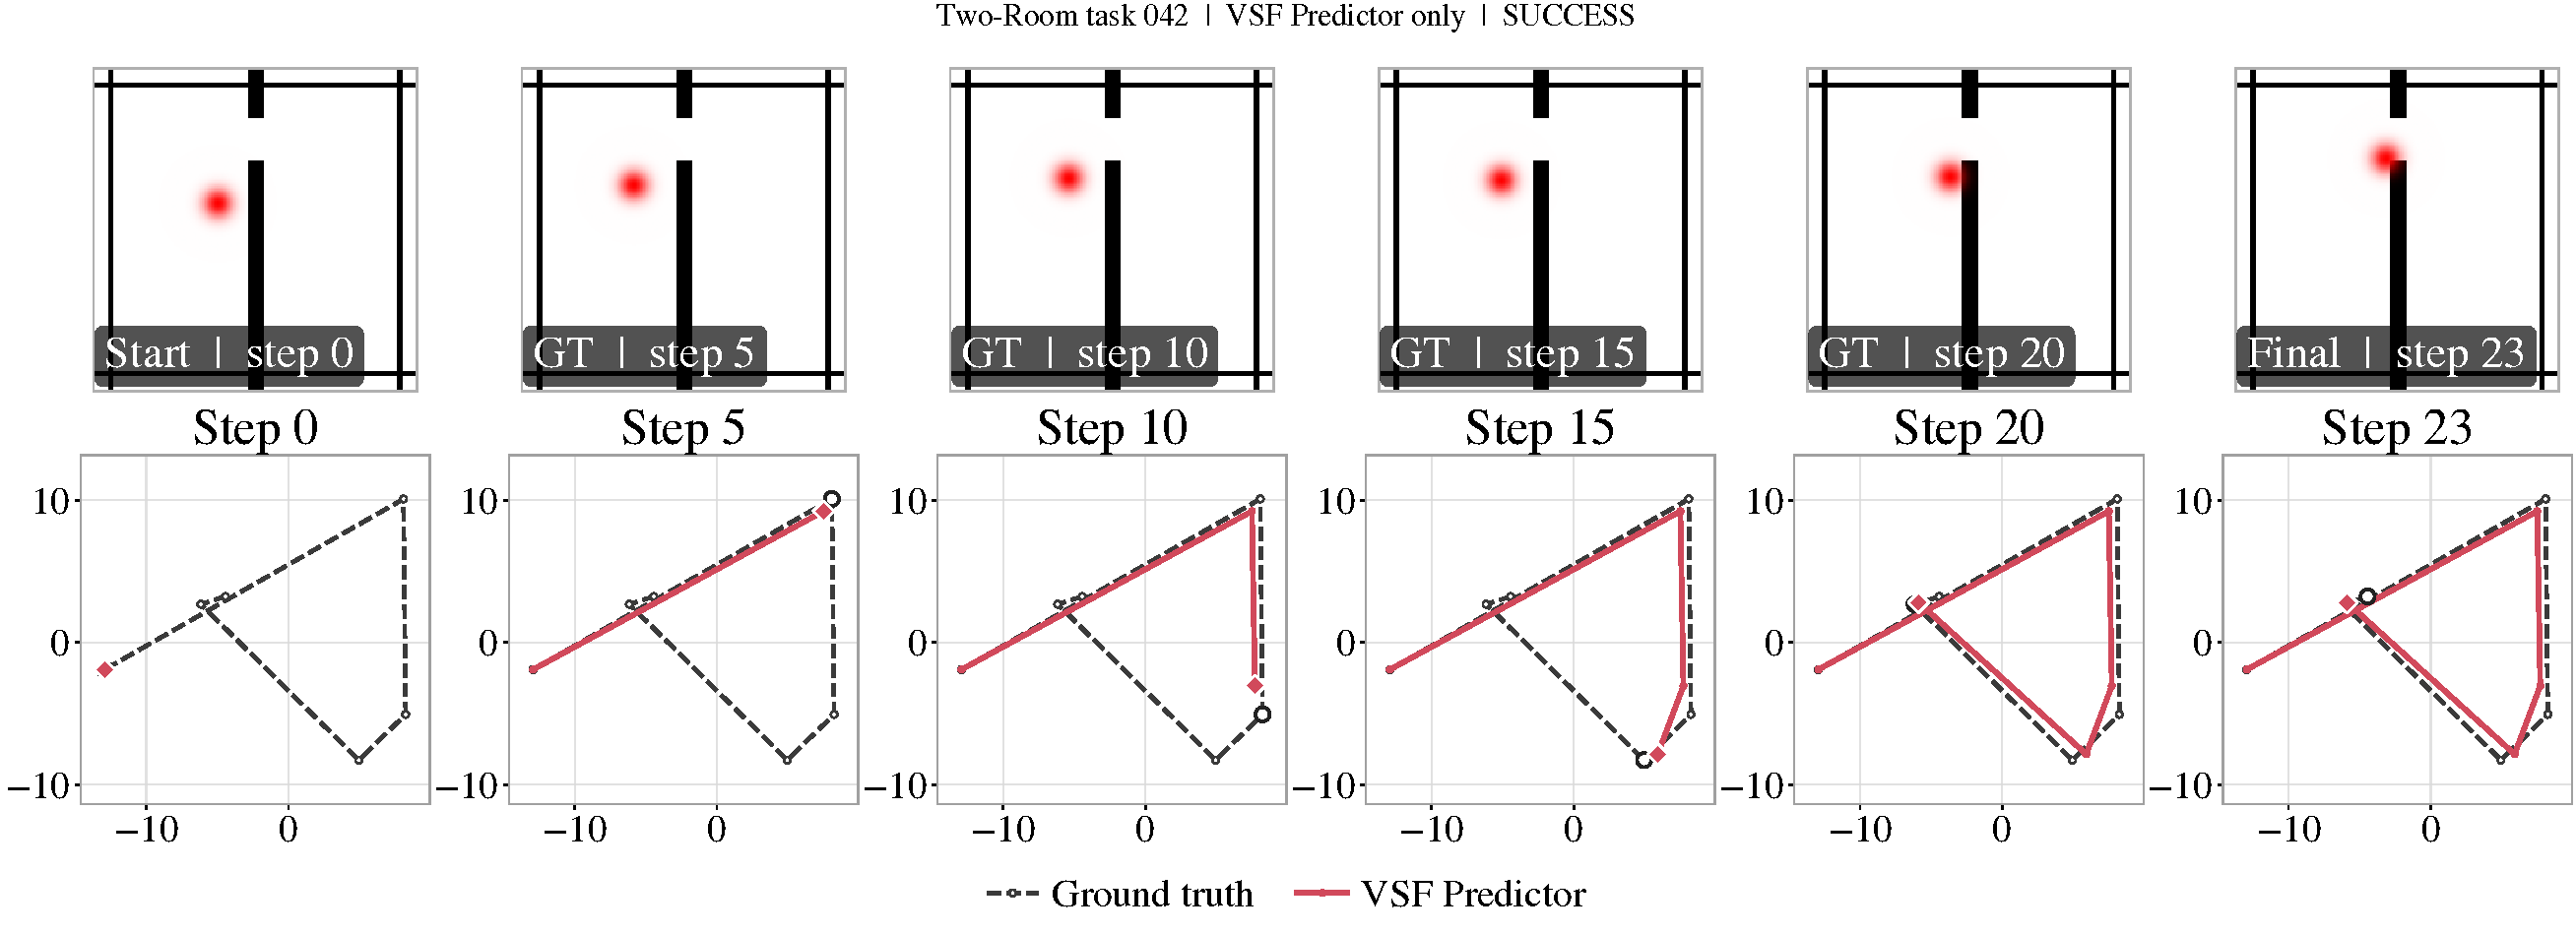
\includegraphics[
    width=\linewidth,
    trim={0bp 0bp 0bp 20bp},
    clip
  ]{figures/wm/tworoom_task_042_vsf_latent_trajectory.pdf}
  \caption{Qualitative TwoRoom result. VSF action-conditioned predicted latent
  trajectory follows the ground-truth trajectory in a successful rollout.}
  \label{fig:wm-vsf-reacher-qualitative}
\end{figure}





\end{document}
